% Options for packages loaded elsewhere
\PassOptionsToPackage{unicode}{hyperref}
\PassOptionsToPackage{hyphens}{url}
\documentclass[
  10pt,
]{article}
\usepackage{xcolor}
\usepackage{amsmath,amssymb}
\setcounter{secnumdepth}{-\maxdimen} % remove section numbering
\usepackage{iftex}
\ifPDFTeX
  \usepackage[T1]{fontenc}
  \usepackage[utf8]{inputenc}
  \usepackage{textcomp} % provide euro and other symbols
\else % if luatex or xetex
  \usepackage{unicode-math} % this also loads fontspec
  \defaultfontfeatures{Scale=MatchLowercase}
  \defaultfontfeatures[\rmfamily]{Ligatures=TeX,Scale=1}
\fi
\usepackage{lmodern}
\ifPDFTeX\else
  % xetex/luatex font selection
  \setmainfont[]{Times New Roman}
  \setmonofont[]{Menlo}
\fi
% Use upquote if available, for straight quotes in verbatim environments
\IfFileExists{upquote.sty}{\usepackage{upquote}}{}
\IfFileExists{microtype.sty}{% use microtype if available
  \usepackage[]{microtype}
  \UseMicrotypeSet[protrusion]{basicmath} % disable protrusion for tt fonts
}{}
\makeatletter
\@ifundefined{KOMAClassName}{% if non-KOMA class
  \IfFileExists{parskip.sty}{%
    \usepackage{parskip}
  }{% else
    \setlength{\parindent}{0pt}
    \setlength{\parskip}{6pt plus 2pt minus 1pt}}
}{% if KOMA class
  \KOMAoptions{parskip=half}}
\makeatother
\usepackage{longtable,booktabs,array}
\usepackage{calc} % for calculating minipage widths
% Correct order of tables after \paragraph or \subparagraph
\usepackage{etoolbox}
\makeatletter
\patchcmd\longtable{\par}{\if@noskipsec\mbox{}\fi\par}{}{}
\makeatother
% Allow footnotes in longtable head/foot
\IfFileExists{footnotehyper.sty}{\usepackage{footnotehyper}}{\usepackage{footnote}}
\makesavenoteenv{longtable}
\usepackage{graphicx}
\makeatletter
\newsavebox\pandoc@box
\newcommand*\pandocbounded[1]{% scales image to fit in text height/width
  \sbox\pandoc@box{#1}%
  \Gscale@div\@tempa{\textheight}{\dimexpr\ht\pandoc@box+\dp\pandoc@box\relax}%
  \Gscale@div\@tempb{\linewidth}{\wd\pandoc@box}%
  \ifdim\@tempb\p@<\@tempa\p@\let\@tempa\@tempb\fi% select the smaller of both
  \ifdim\@tempa\p@<\p@\scalebox{\@tempa}{\usebox\pandoc@box}%
  \else\usebox{\pandoc@box}%
  \fi%
}
% Set default figure placement to htbp
\def\fps@figure{htbp}
\makeatother
\setlength{\emergencystretch}{3em} % prevent overfull lines
\providecommand{\tightlist}{%
  \setlength{\itemsep}{0pt}\setlength{\parskip}{0pt}}

% ICLR-style page: 5.5in text block on US letter, Times, 10pt
\usepackage[letterpaper,left=1.5in,right=1.5in,top=1in,bottom=1in]{geometry}
\usepackage{amsmath,amssymb,amsthm}
\usepackage{graphicx}
\usepackage{booktabs}
\usepackage{longtable}
\usepackage{array}
\usepackage{microtype}
\usepackage[table]{xcolor}
\usepackage{caption}
\usepackage{titlesec}
\usepackage{titling}
\usepackage[colorlinks=true,linkcolor=blue!45!black,urlcolor=blue!45!black,
            citecolor=blue!45!black]{hyperref}
\theoremstyle{plain}
\newtheorem{theorem}{Theorem}
\newtheorem{proposition}[theorem]{Proposition}
\newtheorem{corollary}[theorem]{Corollary}
\theoremstyle{definition}
\newtheorem{assumption}{Assumption}
\setlength{\emergencystretch}{3em}
\providecommand{\tightlist}{\setlength{\itemsep}{0pt}\setlength{\parskip}{0pt}}
\captionsetup{font=small,labelfont=bf}

\titleformat{\section}{\normalfont\large\bfseries}{\thesection}{0.7em}{}
\titleformat{\subsection}{\normalfont\normalsize\bfseries}{\thesubsection}{0.6em}{}
\titleformat{\subsubsection}{\normalfont\normalsize\bfseries\itshape}{\thesubsubsection}{0.6em}{}
\titlespacing*{\section}{0pt}{1.7ex plus .6ex minus .2ex}{1.0ex plus .2ex}
\titlespacing*{\subsection}{0pt}{1.3ex plus .5ex minus .2ex}{0.8ex plus .2ex}
\titlespacing*{\subsubsection}{0pt}{1.1ex plus .4ex minus .2ex}{0.7ex plus .2ex}

\pretitle{\begin{center}\LARGE\bfseries}
\posttitle{\par\end{center}\vskip 0.4em}
\preauthor{\begin{center}\large}
\postauthor{\par\end{center}}
\predate{\begin{center}\normalsize}
\postdate{\par\end{center}\vskip 0.8em}

\newenvironment{iclrabstract}
  {\vspace{0.4em}\begin{center}{\bfseries\scshape Abstract}\end{center}
   \begin{list}{}{\setlength{\leftmargin}{0.45in}\setlength{\rightmargin}{0.45in}}\item[]\relax}
  {\end{list}\vspace{0.6em}}

% wide tables and figures shrink to the measure instead of running off the page
\newcommand{\fitwidth}[1]{\makebox[\linewidth][c]{\resizebox{\ifdim\width>\linewidth\linewidth\else\width\fi}{!}{#1}}}

% Times carries no mathematical glyphs; give those code points a real font
\usepackage{newunicodechar}
\newfontfamily\symfont{STIX Two Math}[Scale=MatchLowercase]
\newunicodechar{ℝ}{{\symfont ℝ}}
\newunicodechar{ℙ}{{\symfont ℙ}}
\newunicodechar{𝔼}{{\symfont 𝔼}}
\newunicodechar{∈}{{\symfont ∈}}
\newunicodechar{⋃}{{\symfont ⋃}}
\newunicodechar{∪}{{\symfont ∪}}
\newunicodechar{⊆}{{\symfont ⊆}}
\newunicodechar{⊂}{{\symfont ⊂}}
\newunicodechar{∝}{{\symfont ∝}}
\newunicodechar{∎}{{\symfont ∎}}
\newunicodechar{≪}{{\symfont ≪}}
\newunicodechar{∼}{{\symfont ∼}}
\newunicodechar{∅}{{\symfont ∅}}
\newunicodechar{₉}{{\symfont ₉}}
\newunicodechar{₅}{{\symfont ₅}}
\newunicodechar{⁻}{{\symfont ⁻}}

\pagestyle{plain}
\setlength{\parskip}{0.45em}
\setlength{\parindent}{0pt}
\usepackage{bookmark}
\IfFileExists{xurl.sty}{\usepackage{xurl}}{} % add URL line breaks if available
\urlstyle{same}
\hypersetup{
  pdftitle={Recursive Axis Conditioning for Diverse Synthetic Data Generation},
  hidelinks,
  pdfcreator={LaTeX via pandoc}}

\title{Recursive Axis Conditioning for Diverse Synthetic Data
Generation}
\author{}
\date{}

\begin{document}
\maketitle

\begin{iclrabstract}

\textbf{Recursive Axis Conditioning} (RAC) generates synthetic corpora
that beat the released state of the art at a twentieth of its budget.
Against Alpaca, PersonaHub and WizardLM Evol-Instruct, scored on
coverage of a held-out human-written reference that no corpus was aimed
at, RAC places \textbf{first of twelve corpora --- 0.4441 against
Alpaca\textquotesingle s 0.3722} at matched evaluated \emph{n}, from
2,400 generator calls against Alpaca\textquotesingle s 52,000, and with
the highest precision in the field (0.973). PersonaHub (50k items) and
WizardLM (143k) both finish below RAC\textquotesingle s 304-item
selective arm.

The score is worth what it buys, and three measurements say what that
is. \textbf{Four hundred RAC items cover more of a held-out human
reference than all 52,002 items of Alpaca} --- a ratio of 130 to 1 ---
and extending the policy to 13,978 items reaches 2.2×
Alpaca\textquotesingle s coverage from 27\% of the items. At matched
pool size, \textbf{7.3× as many held-out queries have a usable nearest
neighbour} as under plain conditioning. And prompting a base model with
retrieved demonstrations, the advantage \emph{grows with every slot
retrieved} --- 1.04×, 1.17×, 1.48×, 2.38× over plain conditioning at k =
1, 2, 4, 8 --- until at eight demonstrations the corpus leads the field
outright, Alpaca included, while low-coverage pools collapse to a third
of their one-shot score. A clustered pool runs out of distinct relevant
demonstrations; a covering one does not. Coverage predicts retrieval
quality at \emph{r} = 0.97 and in-context score at \emph{r} = 0.82.

Two limits deserve the same clarity. Fine-tuning does not follow
(\emph{r} = −0.17): the retrieval-aimed corpus yields the best model on
queries near its own items and the worst on those far from them, and a
gradient step averages the two away. And within a \emph{single} corpus,
subsets differing only in spread are not monotone in coverage, so
coverage ranks corpora on retrieval-shaped tasks without being shown to
be the sole mechanism behind that ranking.

In automatic item generation for psychometrics the margin is larger and
the result is new. Asked a reasonable question ten thousand times, a
strong model returns a bank that is \textbf{73.6\% exact duplicates},
one question repeated 2,726 times, and deduplication does not rescue it:
the next three most frequent items are that same question with one word
changed, with its options reshuffled, and on different numbers. We
replace the assumed enemy-item radius with a measured one, adjudicating
236 item pairs blind to distance and provenance and fitting the crossing
at δ = 0.0354, then apply it to real banks. A naively generated bank of
2,500 items yields \textbf{382 that can coexist on one form, 15.3\% of
nominal capacity}, against 94.9\% for human-written MMLU.
RAC\textquotesingle s bank contains \textbf{no enemy pair at all}, 100\%
usable, and against every synthetic baseline it wins every literal and
latent measure at matched \emph{n} --- mean-centered Vendi 124.8 against
persona conditioning\textquotesingle s 99.7 and naive
prompting\textquotesingle s 7.1, with a 0.000 exact-duplicate rate
against 0.668. Against MMLU itself, written by many authors over years
with editorial review, RAC\textquotesingle s items reuse \emph{less}
language: it wins exact duplication, 4-gram self-repetition and
\emph{n}-gram Vendi, and reaches 69\% of the human
bank\textquotesingle s semantic spread.

The second result is a reversal we did not expect. Corpus objectives
divide into two classes --- covering the space, and packing it so no two
items collide --- and the machinery that is load-bearing for one is
actively harmful to the other, in both directions. Greedy k-center, the
classical packing algorithm, wins min-gap in both of our domains and
finishes \textbf{last on coverage, at a sixth of random}. Orthogonalized
conditioning, which is what makes RAC work under max-min, scores
\textbf{0.2941 on coverage against plain conditioning\textquotesingle s
0.3147}, because steering away from the occupied span steers away from
where the reference measure is densest. The two highest-Vendi selectors
are the two worst covering ones. A diversity number therefore carries no
information until its objective is named, and the same generator loop
must be pointed deliberately: in RAC the objective enters at exactly two
places, how a candidate axis is scored and how one of K candidates is
selected, and everything else is shared.

Underneath both results is one limit. We assume an embedding oracle and
no inverse --- we can compute where the next item ought to land and
cannot decode that point into text --- so RAC steers in language, asking
the generator to name the axes along which its own outputs differ,
ranking them, taking their most-different values, and splitting an
exhausted axis into finer sub-axes that apply only inside the region
that exhausted it. That recursion is the only mechanism we found that
moves the asymptote rather than the constant, because no selection rule
can exceed what the conditional support offers: fifteen numerical checks
confirm that novelty at a fixed prompt decays as \(n^{-1/m}\) in the
conditional dimension rather than \(n^{-1/d}\) in the ambient one, that
a single prompt ε-covers a vanishing \(ε^{d-m}\) fraction, and that only
prompt motion transverse to the occupied span raises the ceiling.
Evidence: \textasciitilde46,000 real generations, \textasciitilde700
rendered images and \textasciitilde200 rendered instrumentals, with
text-embedding similarity predicting rendered-image similarity at only
\textbf{\emph{r} = 0.170}, so every text-side method in this literature
is optimizing a proxy that explains about 3\% of what the reader
receives.

\begin{center}\rule{0.5\linewidth}{0.5pt}\end{center}

\end{iclrabstract}

\subsection{1. Results}\label{1-results}

Synthetic corpora are judged by a measure, and the measure is chosen
before the corpus is. This paper is about building a generator loop that
improves such a measure. The method is \textbf{Recursive Axis
Conditioning} (RAC), and the two measures we take it furthest on are
\textbf{coverage}, which asks the corpus to reach as much of the space
as possible in \emph{n} generator calls, and \textbf{max-min}, which
asks that no two of the \emph{n} items resemble each other. What the
method achieves on each:

\textbf{Coverage of a held-out human-written reference.} Twelve corpora,
matched evaluated \emph{n} = 450, scored by the Naeem et al. (2020)
estimator with reference-side k-NN radii, reported as AUC over k ∈ \{3,
5, 10, 20\}. The radii are a property of the reference alone, so nothing
is tunable per corpus, and no corpus in the table was aimed at the
evaluation half.

{\footnotesize
\begin{longtable}[]{@{}>{\raggedright\arraybackslash}p{\dimexpr 0.3505\linewidth-2\tabcolsep\relax}>{\raggedright\arraybackslash}p{\dimexpr 0.3159\linewidth-2\tabcolsep\relax}>{\raggedright\arraybackslash}p{\dimexpr 0.1697\linewidth-2\tabcolsep\relax}>{\raggedright\arraybackslash}p{\dimexpr 0.1639\linewidth-2\tabcolsep\relax}@{}}
\toprule\noalign{}
rank & corpus & coverage AUC & precision \\
\midrule\noalign{}
\endhead
\bottomrule\noalign{}
\endlastfoot
1 & \textbf{RAC-coverage, retrieval-aimed (2.4k)} & \textbf{0.4441} &
\textbf{0.973} \\
2 & Alpaca (Self-Instruct, 52k) & 0.3722 & 0.87 \\
3 & RAC-coverage, selective 1-of-8 (304) & 0.2591 & 0.93 \\
4 & PersonaHub (50k) & 0.2532 & 0.78 \\
5 & WizardLM Evol-Instruct (143k) & 0.2329 & 0.77 \\
6 & Self-Instruct (reimplemented, same seeds and budget) & 0.2188 & \\
7--9 & budget-matched ablation arms & 0.2102--0.2127 & \\
10--12 & unseeded arms (450 each) & 0.0947--0.1008 & \\
\end{longtable}}

First place, ahead of Alpaca by 19\%, on one twentieth of
Alpaca\textquotesingle s generation budget and with the highest
precision in the field. PersonaHub and WizardLM finish below our
304-item selective arm despite 20--60× the scale.

\textbf{Max-min at matched \emph{n}.} Against five published methods on
two text domains, RAC wins every literal and latent measure. On
psychometric items at \emph{n} = 1,058:

{\footnotesize
\begin{longtable}[]{@{}>{\raggedright\arraybackslash}p{\dimexpr 0.2542\linewidth-2\tabcolsep\relax}>{\raggedright\arraybackslash}p{\dimexpr 0.1154\linewidth-2\tabcolsep\relax}>{\raggedright\arraybackslash}p{\dimexpr 0.1154\linewidth-2\tabcolsep\relax}>{\raggedright\arraybackslash}p{\dimexpr 0.1271\linewidth-2\tabcolsep\relax}>{\raggedright\arraybackslash}p{\dimexpr 0.1413\linewidth-2\tabcolsep\relax}>{\raggedright\arraybackslash}p{\dimexpr 0.1233\linewidth-2\tabcolsep\relax}>{\raggedright\arraybackslash}p{\dimexpr 0.1233\linewidth-2\tabcolsep\relax}@{}}
\toprule\noalign{}
arm & exact-dup ↓ & distinct-2 ↑ & self-repetition ↓ & \emph{n}-gram
Vendi ↑ & centered Vendi ↑ & median NN dist ↑ \\
\midrule\noalign{}
\endhead
\bottomrule\noalign{}
\endlastfoot
naive & 0.668 & 0.114 & 0.855 & 11.8 & 7.1 & 0.000 \\
high temperature & 0.660 & 0.119 & 0.845 & 12.2 & 7.0 & 0.000 \\
Self-Instruct & 0.026 & 0.193 & 0.485 & 288.8 & 59.3 & 0.033 \\
Evol-Instruct & 0.025 & 0.224 & 0.470 & 307.4 & 75.0 & 0.047 \\
persona conditioning & 0.004 & 0.377 & 0.184 & 545.6 & 99.7 & 0.130 \\
\textbf{RAC} & \textbf{0.000} & \textbf{0.429} & \textbf{0.053} &
\textbf{644.3} & \textbf{124.8} & \textbf{0.210} \\
\end{longtable}}

Against human-written MMLU at matched \emph{n} = 1,000, RAC wins exact
duplication, 4-gram self-repetition and \emph{n}-gram Vendi, and reaches
69\% of the human bank\textquotesingle s mean-centered semantic
diversity.

The rest of the paper says what the method is, why the two objectives
need different scoring rules, and what limits both of them.

\subsection{2. Introduction}\label{2-introduction}

Ask a language model for a poem ten times and you get ten poems. Ask it
ten thousand times and you get a few hundred poems and a great deal of
paraphrase. Any fixed conditional distribution behaves this way under
repeated sampling, whatever model supplies it: the distribution has a
shape, and sampling traces that shape ever more densely rather than
expanding it.

The practical version of this is now everywhere. Synthetic training data
is worth what it adds to the training set. An evaluation suite that
clusters in a few families gives false assurance. Test-item banks,
red-team prompt sets, persona corpora and augmentation pipelines all
consume generated text in bulk, and all of them degrade in a way that
per-item quality checks do not detect: every item is fine, and the
collection is redundant. The failure is a property of the collection,
and the corpora shipped today have it badly. Asked a reasonable
psychometric question ten thousand times, a strong model returns a bank
that is 73.6\% byte-identical duplicates, and of a 2,500-item sample
only 382 items can legally coexist on one exam form.

This paper presents \textbf{Recursive Axis Conditioning} (RAC), a
generation loop that fixes this well enough to beat the released state
of the art at a twentieth of its budget, and reports two results from
building it.

The first is that the loop works, and by margins that do not depend on
scale. Against Alpaca, PersonaHub and WizardLM Evol-Instruct on coverage
of a held-out human reference, RAC places first of twelve corpora from
2,400 generator calls against Alpaca\textquotesingle s 52,000. On
psychometric item generation it produces a bank with no enemy pair at
all at a judged radius, where the naive bank yields 15.3\% of its
nominal capacity and human-written MMLU yields 94.9\%.

The second result was not what we set out to find. Corpus objectives
fall into two classes: \emph{covering} the reachable space, and
\emph{packing} it so that no two items collide. These are usually spoken
of interchangeably, as two ways of asking for a diverse corpus. They are
not interchangeable, and the machinery that is load-bearing for one is
actively harmful to the other in both directions. Greedy k-center, the
classical packing algorithm, wins the min-gap metric in both of our
domains and finishes last on coverage, at a sixth of random.
Orthogonalized conditioning, the component that makes RAC work under
packing, \emph{reduces} coverage below plain conditioning when carried
across. The two highest-Vendi selectors we measure are the two worst
covering ones. Section 4 develops this, and it is the reason the same
loop has to be pointed deliberately rather than tuned once and reused.

Underneath both results is a single limit, which §5 makes precise: no
selection rule can outrun the conditional support of the generator it is
drawing from, so the only move that changes the asymptote is one that
widens that support.

\subsubsection{2.1 The oracle asymmetry}\label{21-the-oracle-asymmetry}

We assume throughout:

\begin{quote}
\textbf{Assumption (embedding oracle, no inverse).} We have access to
\emph{E}: Text → ℝ\emph{D}, computable on demand. We have \textbf{no}
\emph{E}−1: ℝ\emph{D} → Text.
\end{quote}

This is the structural fact that shapes the entire design, and it is
worth dwelling on because it is easy to forget when writing down
objectives. Given \emph{Xn} we can compute, exactly and cheaply, the
point in ℝ\emph{D} that would most improve any of our diversity measures
--- the direction of least occupied spectral energy, the centre of the
largest empty ball, the point maximizing marginal coverage. Knowing that
point is worth nothing on its own. There is no procedure that turns a
target embedding back into a poem.

Consequently the system cannot \emph{solve} for its next item. It can
only:

\begin{enumerate}
\def\labelenumi{\arabic{enumi}.}
\tightlist
\item
  \textbf{propose} (sample from \emph{p}(· \textbar{} \emph{x}) for some
  prompt \emph{x} we are able to write;
\item
  \textbf{measure}) embed the proposals and score them;
\item
  \textbf{select} --- keep one.
\end{enumerate}

All of the control we have is therefore in step 1, in the choice of
\emph{x}, and that choice is expressible only in language. This is why
the latent variables in our system are \emph{language-valued} (named
axes with named levels), rather than continuous codes: they are the only
handles that reach the generator. It is also why the axis scoring of §6
exists. \textbf{The axis scoring is a surrogate for the missing
inverse.} Since we cannot decode the direction we want to travel, we
instead score the language-valued conditions we \emph{can} write by how
nearly their induced output distributions point that way.

\subsubsection{2.2 Contributions}\label{22-contributions}

\begin{itemize}
\tightlist
\item
  \textbf{A generator loop that improves a chosen measure} (§6).
  Language-valued axes elicited from the generator, ranked by a scoring
  rule, with the exhausted ones split recursively into conditional
  sub-axes. The measure enters at two points only: how an axis is
  scored, and how one of K candidates is selected, so pointing the loop
  at a different measure means changing those two and nothing else.
\item
  \textbf{A theory of what limits both} (§5). Conditioned on a fixed
  prompt, the output concentrates on a submanifold of dimension \emph{m}
  far below the dimension \emph{d} of the reachable space, and the
  consequences are the same for packing and for covering.
\item
  \textbf{Evidence that the measure has to be named} (§4). Greedy
  k-center wins min-gap in both domains and finishes last on coverage,
  and each measure\textquotesingle s characteristic tool damages the
  other\textquotesingle s score, so "diverse" without a named measure
  carries no information.
\item
  \textbf{Head-to-head against released corpora} (§7), on a scale-free
  estimator against a reference no corpus was aimed at, and against a
  human-written exam bank under a judged enemy-item radius.
\end{itemize}

\subsection{3. Related work}\label{3-related-work}

\textbf{Diversity metrics.} The Vendi Score (Friedman \& Dieng, 2022) is
the exponential of the von Neumann entropy of a normalized similarity
matrix, interpretable as an effective number of distinct items. We use
it throughout, with a computational note: under a linear kernel on
unit-normalized embeddings, the \emph{n} × \emph{n} Gram matrix and the
\emph{D} × \emph{D} second-moment matrix share their nonzero spectrum,
so the score costs \emph{O}(\emph{nD}² + \emph{D}³), rather than
\emph{O}(\emph{n}³). We verify this to machine precision (max eigenvalue
mismatch 1.1 × 10−16). This matters for our setting specifically: an
infinite-horizon method needs an evaluation whose cost does not grow
superlinearly in the thing it is evaluating.

\textbf{Selection and subset choice.} Determinantal point processes
model repulsion via volume in feature space. Farthest-point /
\emph{k}-center greedy is the classical max--min packing heuristic and
we use it as a baseline (\texttt{fps\_post}) and, at the level of axis
values, as a component (§6.4). SemDeDup-style near-duplicate removal at
a fixed radius appears as \texttt{dedup\_post}. All of these are
\emph{post hoc} selectors over a fixed pool, which is exactly their
limitation in our setting: they cannot change what is in the pool.

\textbf{Quality-diversity.} MAP-Elites and its descendants maintain an
archive indexed by hand-designed behavior descriptors, seeking an elite
per cell. Our axis lattice is a close relative, with two differences
that matter here: the descriptors are \emph{elicited from the generator
rather than designed by us}, and the lattice \emph{refines itself} when
a cell saturates, so the archive\textquotesingle s resolution is not
fixed in advance.

\textbf{Mode collapse in instruction-tuned models.} Repeated sampling
from aligned models is well documented to produce low lexical and
semantic entropy relative to base models. We take this as our empirical
starting point and model it explicitly as skewed mixture weights over
style modes.

\textbf{Novelty search.} Novelty search in evolutionary computation
rewards behavioral distance from an archive. Our repulsion term is a
direct analogue, operating over an archive of embeddings rather than of
behavior descriptors.

\textbf{Coverage.} The covering objective is treated below (maximizing
the volume of a union of ε-balls at a \emph{finite} budget), which is
submodular where max--min is not. §4 relates the two.

\textbf{Submodular maximization.} The (1 − 1/e) greedy guarantee for
monotone submodular objectives is Nemhauser, Wolsey \& Fisher (1978);
hardness of beating it for max-coverage is Feige (1998). Lazy greedy
(Minoux 1978) and stochastic greedy (Mirzasoleiman et al. 2015) make
greedy cheap; sieve-streaming (Badanidiyuru et al. 2014) gives the
single-pass regime our sequential setting approximates. Facility
location (of which our pool objective is the thresholded special case)
is the standard submodular model of "representativeness" in data
summarization (Lin \& Bilmes 2011).

\textbf{Packing vs covering, k-center vs k-median.} Farthest-point
traversal (Gonzalez 1985) 2-approximates k-center --- the packing
objective this paper streams, while k-median/facility-location minimizes
\emph{average} service distance and behaves like our coverage objective
(measure-weighted, bulk-first, outlier-indifferent). Coreset
constructions (Har-Peled \& Mazumdar 2004) make the same distinction: an
ε-coreset for k-median weights by mass, a k-center net does not. Our
contribution is not new theory for these objects but the identification
of \emph{which one the corpus-construction product requirement actually
is}, plus measurement of what optimizing the wrong one costs.

\textbf{Quality-diversity search.} MAP-Elites (Mouret \& Clune 2015)
maintains an "illuminated map": one elite per cell of a hand-designed
behavior space --- equal allocation over a fixed grid, in our
vocabulary, with quality as the within-cell objective. Our method
differs in that cells are elicited from the generator and refined
recursively rather than fixed, allocation is marginal-gain-driven rather
than one-per-cell, and coverage is measured against a reachable
distribution rather than a designer-set grid; §5.11\textquotesingle s
equal-allocation row quantifies what the fixed-grid choice costs at
small ε.

\textbf{Diversity metrics and dedup.} The Vendi score (Friedman \& Dieng
2022) is our spectrum-level diversity readout, computed at O(nD² + D³)
via the Gram trick as in the packing objective. SemDeDup (Abbas et al.
2023) removes semantic near-duplicates from web-scale corpora --- the
deletion-side mirror of our selection problem: both spend a budget to
maximize non-redundant semantic territory. DPPs (Kulesza \& Taskar 2012)
give probabilistic diverse selection; exact DPP sampling scales poorly
in n and optimizes a determinant (volume) rather than covered measure,
though greedy MAP-DPP behaves similarly to facility-location greedy in
practice.

\textbf{Eval-suite construction.} Perez et al. (2022) generate
evaluations with LMs at scale; red-teaming work (Ganguli et al. 2022)
documents exactly the clustering-into-attack-families failure that
motivates a coverage objective for safety suites.

\textbf{Synthetic instruction corpora, and the baselines we compare
against.} Self-Instruct (Wang et al. 2023) bootstraps instructions from
a seed pool with few-shot exemplars and a ROUGE-L similarity filter; the
released Stanford Alpaca corpus (Taori et al. 2023, 52,002 items) is its
canonical output. Evol-Instruct / WizardLM (Xu et al. 2023) instead
\emph{mutates} existing instructions with depth and breadth evolution
operators, released as WizardLM\_evol\_instruct\_V2 (143,000 items).
Persona-Hub (Ge et al. 2024) conditions generation on a catalogue of
\textasciitilde1B personas, releasing 50,000 persona-synthesized
instructions; it is the closest published relative of latent-axis
conditioning, differing in that its catalogue is mined at scale and
flat, where our axes are elicited from the generator and refined into a
tree. AttrPrompt (Yu et al. 2023) similarly conditions on attribute
dimensions. We compare against the released artifacts of the first three
(§7.7), rather than against reimplementations, since a reimplementation
can be weak in ways that flatter us. On the selection side our baselines
are the standard ones for diverse subset choice: SemDeDup (Abbas et al.
2023), farthest-point traversal (Gonzalez 1985), and greedy MAP
inference for DPPs (Kulesza \& Taskar 2012; Chen, Zhang \& Zhou 2018).

\subsection{4. What helps one objective hurts the
other}\label{4-what-helps-one-objective-hurts-the-other}

Covering and packing are routinely treated as two phrasings of one goal.
On real corpora they rank methods almost oppositely, and each
one\textquotesingle s characteristic tool costs the other measurably.
This section establishes that, then explains why it happens and what
follows for the loop.

Both objectives are stated carefully first, since the reversal is easy
to mistake for a tuning artifact. Coverage is the right question when
the corpus stands for a population, as an evaluation suite or a training
set does: what fraction of the space has an exemplar? Packing is the
right question when a single collision is a defect on its own, as in an
exam bank where two items testing the same rule are a security failure
whatever the other items look like. Both are named below, and then
measured against each other.

\subsubsection{4.1 Max-min, stated}\label{41-max-min-stated}

Under an unbounded horizon the objective is a two-term score evaluated
against everything generated so far. Let \emph{E} be an embedding oracle
and let \emph{Xn} = \{\emph{x}1, \ldots, \emph{xn}\} be the corpus. For
a candidate \emph{c},

\[
J_\lambda(c \mid X_n) \;=\; \lambda \cdot \underbrace{\frac{1}{n}\sum_{i=1}^{n}\lVert E(c) - E(x_i)\rVert}_{\text{anchor: keep it typical}} \;-\; (1-\lambda)\cdot \underbrace{\min_{i \le n} \lVert E(c) - E(x_i)\rVert}_{\text{repulsion: keep it new}}
\]

and we accept the candidate minimizing \emph{J}λ. The anchor keeps
generation on the manifold, the repulsion pushes it away from what
already exists, and λ trades them off. Both terms are cheap to maintain
online: the anchor decomposes into distance-to-centroid plus a
candidate-independent constant, so ranking by it is \emph{O}(\emph{D})
per candidate and \emph{O}(1) in \emph{n}, and the repulsion needs one
nearest-neighbour query, which we bound by subsampling.

Neither term is where the difficulty lives, as §5 shows. Both behave
predictably; what does not is the set of candidates they are evaluated
on.

\subsubsection{4.2 The reachable manifold and the conditional
slice}\label{42-the-reachable-manifold-and-the-conditional-slice}

Let \emph{M} ⊂ ℝ\emph{D} be the reachable semantic manifold, dim
\emph{M} = \emph{d}: the set of embeddings of texts the generator could
produce under \emph{some} prompt. For a fixed prompt \emph{x}, let
\emph{Sx} ⊆ \emph{M} be the support of \emph{E}\#\emph{p}(· \textbar{}
\emph{x}), with dim \emph{Sx} = \emph{m}.

The empirical claim behind everything below is that \textbf{\emph{m} ≪
\emph{d}}. A prompt fixes topic, stance, form, register, and rhetorical
strategy; what remains free is a low-dimensional residue --- some
lexical choice, some ordering, some surface variation. Our live pilot
supports this directly: 60 poems generated from an identical naive
prompt have a median nearest-neighbour cosine similarity of 0.911 and a
Vendi Score of 2.55, meaning sixty samples behave like roughly two and a
half distinct items.

Throughout, \emph{B}(\emph{x}, \emph{r}) is the ball of radius \emph{r}
and we write \emph{gn} for the min-gap of a fresh draw against a corpus
of size \emph{n}.

\subsubsection{4.3 Coverage, stated}\label{43-coverage-stated}

Fix an embedding map φ into R\^{}D (we use unit-normalized 768-d
embeddings), and a radius ε \textgreater{} 0. The generator, prompted in
whatever ways the pipeline can reach, induces a \emph{reachable
distribution} μ over R\^{}D: the pushforward of everything the generator
can actually be made to produce. Given a budget n, choose a set S =
\{x\_1, \ldots, x\_n\} of generated items to maximize the covered
measure

\(F_{\mu,\varepsilon}(S) = \mu\!\left(\bigcup_{x \in S} B(x,\varepsilon)\right)\),

the probability that a fresh draw from the generator lands within ε of
some chosen item. Equivalently, S should be an ε-net for as much of μ as
the budget allows. Three deliberate choices:

\begin{itemize}
\tightlist
\item
  \textbf{Coverage of the reachable space, not of R\^{}D.} Balls in
  empty space cover Lebesgue volume but no behavior. Measuring against μ
  makes the metric mean "fraction of what the generator can do that the
  corpus has an exemplar of", which is the product requirement for an
  eval suite. The denominator is therefore stated next to every coverage
  number; where corpora built by different methods are compared, it is a
  held-out human-written reference identical for all of them (§7.7).
\item
  \textbf{ε is a resolution parameter, not a nuisance.} Small ε asks for
  exemplars of fine behavioral distinctions; large ε only for one
  exemplar per coarse region. Every result below names the radius, or
  the range of radii, it is reported at, because the ranking of methods
  changes with ε.
\item
  \textbf{Quality is a constraint, not part of the objective.} An item
  that covers new territory but fails a quality/typicality bar is not an
  asset, so the judge gate rejects it regardless of the gain it would
  have scored (§6.6).
\end{itemize}

\textbf{The oracle asymmetry.} One assumption structures everything
downstream: we have an embedding oracle E: text → R\^{}D, and \emph{no
inverse}. There is no E⁻¹ that decodes a target point back into text. We
can compute exactly where in embedding space the next item should land
--- the largest uncovered region, the trailing eigenspace, but we cannot
manufacture an item that lands there. The only handles a pipeline has
are (a) language-valued latent conditioning that \emph{steers} the
generator\textquotesingle s proposal distribution, and (b) selection
among sampled candidates. This is why the architecture is
propose--measure--select rather than solve, and it has two consequences
we state as propositions:

\begin{quote}
\textbf{Proposition 1 (no direct construction).} Coverage-optimal point
sets are not directly constructible. The greedy (1 − 1/e) guarantee
(§5.7) holds relative to the best subset of the \emph{proposal
distribution\textquotesingle s support}, not of R\^{}D; the difference
between what an unconstrained selector could cover and what a
proposal-limited selector can is a \emph{reachability gap}, which is a
property of the generator-plus-conditioning stack, not of the selection
algorithm. We measure it directly in §5.11.
\end{quote}

\begin{quote}
\textbf{Proposition 2 (conditioning as surrogate inverse).}
Language-valued conditioning is the only available surrogate for E⁻¹:
choosing which axis to condition on next is choosing which \emph{slice}
of the reachable manifold the next candidates will be sampled from, so a
axis scoring that ranks axes by where their slices land (§6.6) is
precisely an approximate inverse --- it maps "where we want mass" to
"which words to condition on".
\end{quote}

\subsubsection{4.4 Where they coincide}\label{44-where-they-coincide}

\textbf{Where they are dual.} For radius ε, a \emph{maximal} ε-packing
is automatically an ε-covering: any uncovered point could have been
added to the packing. We confirm this numerically on 3,000 held-out
human instructions --- at every ε tested, the greedy maximal packing
covers 100.0\% of the set, and the classical sandwich N\_cov(ε) ≤
N\_pack(ε) ≤ N\_cov(ε/2) holds. Max-min run to maximality \emph{is} a
covering algorithm, and greedy k-center 2-approximates the covering
\textbf{radius}.

\textbf{Where they are not.} That duality concerns the worst-case
radius: the distance from the least-covered point to its nearest center.
The coverage that matters for synthetic data is
\textbf{measure-weighted} --- what fraction of the reference
distribution lies within reach, and the two come apart exactly when the
measure is non-uniform, which it always is. k-center is driven by
outliers: every isolated point sets the max and so commands a center.
Measure-weighted coverage is driven by mass: an outlier is worth its own
measure and no more. At a budget far below what the space needs, the
prescriptions are opposite, and that is the entire content of our
k-center result (first on min-gap, last on coverage). The true dual of
measure-weighted coverage is fractional set cover, whose primal is
submodular; max-min is not.

\textbf{What the duality still buys: packing calibrates, covering
places.} Even where packing is the wrong way to \emph{place} points, it
is the right way to \emph{choose the scale}. Define ε*(n) as the radius
at which a maximal packing of the reference has about n points --- the
finest resolution an n-item corpus can deliver. Measured on the held-out
human reference: ε*(100) = 0.549, ε*(450) = 0.472, ε*(1000) = 0.418.
This retroactively diagnoses our failed fixed-ε comparison with more
precision than "the ε was too small": its ε sat at the 2nd percentile of
pairwise distances \emph{regardless of budget}, while a 450-item corpus
genuinely supports about the 2.6th percentile --- the error was choosing
resolution independently of n. Protocol: calibrate ε by packing, then
place by greedy marginal coverage against the measure.

\textbf{The ceiling decomposition.} In a generative setting, selection
cannot cover what generation never proposed. We therefore report every
coverage number as achieved = ceiling × efficiency, where the ceiling is
the coverage of the reference by the union of \emph{all} candidates the
generator produced, and efficiency is the fraction of that ceiling the
selector captured. A low ceiling with high efficiency says the axes are
too narrow and more search is wasted --- only support expansion
(recursive refinement) can help; the reverse says the selector is the
problem. Without the split, "we lost on coverage" gives no indication of
what to change.

\subsubsection{4.5 Coverage is not
packing}\label{45-coverage-is-not-packing}

Max-min selection (choose the candidate farthest from the accepted set)
is the greedy algorithm for the k-center / packing objective, and this
paper paper shows it is the right \emph{shape} of objective for an
unbounded stream once a typicality anchor keeps it on-manifold. At a
finite budget against a fixed μ the two objectives pull apart:

\begin{itemize}
\tightlist
\item
  k-center cares about the worst-covered \emph{point of S itself}; its
  optima push to the boundary of the support and place points in regions
  of vanishing measure (an outlier is far from everything, so packing
  \emph{rewards} it), and under a fixed budget every such item is a ball
  spent covering ≈ 0 measure.
\item
  Maximum coverage / facility-location-type objectives weight territory
  by measure: a second exemplar in a heavy mode can be worth more than a
  first exemplar of a negligible one, and junk is worth nothing because
  μ puts almost nothing near it.
\end{itemize}

§7.14 isolates the contrast with no generator in the loop: on one shared
candidate set, greedy-coverage covered 0.528 of a held-out pool where
farthest-point packing covered 0.143, while packing\textquotesingle s
min-gap (1.44) beat greedy\textquotesingle s (0.577) by 2.5×. Neither is
"better"; they optimize different functionals, and §5.11 shows the same
double dissociation with the full generation loop in place.

\subsubsection{4.6 The reversal,
measured}\label{46-the-reversal-measured}

In a leakage-free selection benchmark (one shared candidate pool, budget
matched at 700 and 1,896 generations respectively, selector shown only
an estimation half of the reference and scored on a disjoint held-out
half):

{\footnotesize
\begin{longtable}[]{@{}>{\raggedright\arraybackslash}p{\dimexpr 0.4305\linewidth-2\tabcolsep\relax}>{\raggedright\arraybackslash}p{\dimexpr 0.1808\linewidth-2\tabcolsep\relax}>{\raggedright\arraybackslash}p{\dimexpr 0.2140\linewidth-2\tabcolsep\relax}>{\raggedright\arraybackslash}p{\dimexpr 0.1747\linewidth-2\tabcolsep\relax}@{}}
\toprule\noalign{}
selector & DALL·E coverage & psychometric coverage & DALL·E min-gap \\
\midrule\noalign{}
\endhead
\bottomrule\noalign{}
\endlastfoot
coverage-greedy (ours) & \textbf{0.4829} & \textbf{0.3901} & 0.299 \\
coverage-stream (ours) & 0.4200 & 0.3785 & 0.283 \\
ROUGE-L filter (Self-Instruct) & 0.4629 & 0.3575 & 0.208 \\
SemDeDup & 0.4600 & 0.3575 & 0.336 \\
random & 0.4629 & 0.3533 & 0.198 \\
MAP-DPP greedy & 0.3829 & 0.0988 & 0.402 \\
k-center (Gonzalez) & 0.4114 & 0.0557 & \textbf{0.491} \\
\end{longtable}}

\textbf{k-center wins min-gap outright in both domains and finishes last
on coverage}, at 0.0557 against random\textquotesingle s 0.3533 in the
psychometric domain --- a sixth of what random selection achieves. The
two highest-Vendi selectors (k-center and MAP-DPP) are the two worst
covering ones. A practitioner who reads "diversity" off a Vendi score
and deploys the selector that maximizes it will get a corpus that covers
less of the space than picking at random.

\subsubsection{4.7 Why the scoring rule has to
fork}\label{47-why-the-scoring-rule-has-to-fork}

The four factors are shared but two of them invert:

{\footnotesize
\begin{longtable}[]{@{}>{\raggedright\arraybackslash}p{\dimexpr 0.3802\linewidth-2\tabcolsep\relax}>{\raggedright\arraybackslash}p{\dimexpr 0.3049\linewidth-2\tabcolsep\relax}>{\raggedright\arraybackslash}p{\dimexpr 0.3149\linewidth-2\tabcolsep\relax}@{}}
\toprule\noalign{}
& max-min / packing & coverage / covering \\
\midrule\noalign{}
\endhead
\bottomrule\noalign{}
\endlastfoot
the ask & no two items alike, in \emph{n} turns & reach as much as
possible, in \emph{n} turns \\
governed by & the closest pair & the bulk \\
submodular & no & yes, so greedy carries (1 − 1/e) \\
classical kin & k-center & facility location \\
\textbf{spread(a)} & \textbf{min} distance between level centroids &
\textbf{measure-weighted mean} distance \\
\textbf{headroom(a)} & levels not yet \textbf{used} & measure not yet
\textbf{covered} \\
value selection & \texttt{farthest\_levels} (max-min subset) &
\texttt{coverage\_levels} (greedy marginal gain) \\
failure mode & chases outliers into off-manifold junk & leaves the
frontier empty \\
\end{longtable}}

The behavioural difference is visible on a two-line test. Given an axis
with three tightly-clustered common levels and one rare outlying level,
\texttt{farthest\_levels} picks the outlier \textbf{first} and
\texttt{coverage\_levels} picks a cluster centre first and the outlier
second. That is k-center versus facility location, reproduced inside the
axis axis scoring, and it is the mechanism behind the table above.

\subsubsection{4.8 The ablation that shows the
fork}\label{48-the-ablation-that-shows-the-fork}

§7 compares RAC-coverage with the released Alpaca, PersonaHub and
WizardLM corpora under a controlled protocol (same 175 human seeds, same
generator, budget matched in generator calls, evaluation on a reference
half nothing ever read). RAC-coverage places first of twelve --- 0.4441
against Alpaca\textquotesingle s 0.3722, at one-twentieth of
Alpaca\textquotesingle s budget, with the field\textquotesingle s
highest precision. Two rows of its ablation matter to this joint paper
beyond the ranking.

First, \textbf{the orthogonalization row}. The configuration applying
the packing side\textquotesingle s orthogonalized conditioning to the
coverage objective scores 0.2941, below plain
conditioning\textquotesingle s 0.3147: orthogonalization steers
generation away from the occupied span, which is away from the
reference-dense core coverage is paid to fill. Each
part\textquotesingle s load-bearing tool, applied to the
other\textquotesingle s objective, reduces performance. The two scoring
rules fork because they must.

Second, \textbf{the Vendi row}. The winning coverage corpus has the
\emph{lowest} mean-centered Vendi of any configuration in its cohort
(62.1; density 1.69): it spends items where the reference measure is,
near-duplicates included. A single "diversity score" would rank the
coverage winner last. There is no one number; there are two objectives.

\subsubsection{4.9 What both classes
share}\label{49-what-both-classes-share}

Both are limited by the same thing, and neither optimizer can fix it.
Coverage of a reachable manifold and packing within one are both bounded
by the reachable manifold\textquotesingle s dimension, which is set by
how far the prompt can move the generator --- §5. Both need the same
typicality constraint to be well-posed, since a novelty-seeking score
can otherwise be satisfied by output that has left the manifold
altogether. And both are measured through an embedder whose geometry can
invert the result: we report a cross-corpus coverage comparison in which
our worst corpus by every other measure (19.8\% exact duplicates) scores
the \textbf{highest} coverage, 50× a published corpus\textquotesingle s,
because at an ε in the 2nd percentile of reference distances the metric
rewards centrality rather than spread.

\subsubsection{4.10 Practical guidance}\label{410-practical-guidance}

\begin{enumerate}
\def\labelenumi{\arabic{enumi}.}
\tightlist
\item
  \textbf{Say which objective you mean.} They are different problems
  with different optimal policies, and the vocabulary ("diverse",
  "varied") does not distinguish them.
\item
  \textbf{Count exact duplicates before computing anything.} A 72\%
  duplicate rate makes every distance statistic a statistic about
  duplication.
\item
  \textbf{Publish the pairwise-similarity distribution} your kernel
  operates on. Mean pairwise cosine was 0.883 in one of our corpora and
  0.444 in another with the same embedder; an ε or a Vendi score means
  nothing without it.
\item
  \textbf{Measure at the level of the artifact you ship.} Text-embedding
  similarity explains \textasciitilde2\% of the variance in whether
  rendered images look alike.
\item
  \textbf{Report the procedure with the number.} Our own framework
  changed three times during this work; every result in this paper is
  tagged with the procedure that produced it.
\end{enumerate}

\subsection{5. Theory: the limit both classes
share}\label{5-theory-the-limit-both-classes-share}

Nothing below depends on which measure was chosen. The results in this
section bound what a fixed prompt can reach at all, and a measure
computed on the resulting corpus inherits that bound whatever it is
measuring. The first group concerns the conditional support and applies
to any selection rule; the second concerns the covering functional in
particular, and is what makes greedy selection defensible when coverage
is the measure.

\subsubsection{5.1 Saturation at a fixed
prompt}\label{51-saturation-at-a-fixed-prompt}

\begin{quote}
\textbf{Theorem 1.} Let \emph{Xn} be \emph{n} i.i.d. draws from a
distribution with density bounded above and below on an
\emph{m}-dimensional manifold \emph{S}. For a fresh draw \emph{c} from
the same distribution, 𝔼{[}\emph{gn}{]} = Θ(\emph{n}−1/\emph{m}).
\end{quote}

\emph{Proof sketch.} ℙ(\emph{gn} \textgreater{} \emph{r}) = ℙ(no sample
in \emph{B}(\emph{c}, \emph{r})) = (1 − μ(\emph{B}(\emph{c},
\emph{r})))\emph{n}, and μ(\emph{B}(\emph{c}, \emph{r})) =
Θ(\emph{r}\emph{m}) by density bounds on an \emph{m}-manifold. So
ℙ(\emph{gn} \textgreater{} \emph{r}) ≈ exp(−\emph{n}Θ(\emph{rm})), which
transitions at \emph{r} = Θ(\emph{n}−1/\emph{m}); integrating the tail
gives the expectation. ∎

The content is the exponent. With \emph{d} = 32, a naive reading
predicts \emph{n}−1/32 --- essentially flat, novelty never exhausted.
The true rate at \emph{m} = 3 is \emph{n}−1/3, which is roughly a 10×
loss of headroom per 1000× of corpus. Measured slopes: −0.472 (\emph{m}
= 2), −0.309 (\emph{m} = 3), −0.195 (\emph{m} = 5), against −0.5,
−0.333, −0.2. The \emph{m} = 2 case sits slightly above its asymptote at
these \emph{n}, as expected for a rate with logarithmic corrections.

\begin{quote}
\textbf{Corollary 1.1 (oversampling is not a strategy).} Drawing
\emph{K} candidates and keeping the most novel multiplies the expected
gap by Θ(\emph{K}1/\emph{m}) at best. To recover the headroom lost by a
1000× larger corpus, \emph{K} must grow by 1000.
\end{quote}

Verified at \emph{m} = 3: best-of-8 yields a gain of 2.19 against
\emph{K}1/3 = 2.00. Selection is a constant-factor fix to an asymptotic
problem.

\subsubsection{5.2 The slice deficit}\label{52-the-slice-deficit}

\begin{quote}
\textbf{Theorem 2.} If \emph{m} \textless{} \emph{d}, then
vol\emph{d}(\emph{Sx}) = 0, and the fraction of \emph{M} within ε of
\emph{Sx} is Θ(ε\emph{d}−\emph{m}).
\end{quote}

\emph{Proof sketch.} The ε-neighbourhood of an \emph{m}-dimensional set
in \emph{d} dimensions is a tube of volume Θ(ε\emph{d}−\emph{m}) ·
vol\emph{m}(\emph{Sx}) for ε below the reach of \emph{Sx}. Dividing by
vol\emph{d}(\emph{M}) gives the claim. ∎

Measured at \emph{d} = 8, \emph{m} = 2: fitted exponent 5.06 against a
predicted 6, with covered fractions falling 0.051 → 0.0001 as ε goes 0.5
→ 0.12. The fitted exponent sits below prediction because at the larger
ε the tube is no longer thin relative to the manifold, which flattens
the low-ε end of the fit; the qualitative claim (coverage collapsing
polynomially in ε with a large exponent) is unambiguous.

The practical reading is severe. \textbf{A single prompt, sampled
infinitely often, covers essentially none of what the model could
write.} Not "less than we would like" --- a fraction that goes to zero
polynomially as the resolution of interest sharpens.

\subsubsection{5.3 Transversality: which prompt motion
helps}\label{53-transversality-which-prompt-motion-helps}

Let a prompt schedule induce slices \emph{S}1, \ldots, \emph{SP}. Write
\emph{V}occ for the span of the corpus\textquotesingle s dominant
directions.

\begin{quote}
\textbf{Theorem 3.}
\(\dim\!\left(\bigcup_j S_j\right) = \min\!\left(d,\; m + \operatorname{rank}\{c_j - c_1\}\right)\),
where \(c_j\) is the centre of \(S_j\). In particular, displacements
lying inside \(\operatorname{span}(S_1)\) contribute nothing to the
union\textquotesingle s dimension.
\end{quote}

\emph{Proof sketch.} The union is contained in the affine hull of the
slice frame plus the span of the centre displacements; dimensions add up
to that cap, and a displacement already inside the
slice\textquotesingle s own span adds no new direction. ∎

Measured via participation ratio of the union\textquotesingle s
covariance spectrum: parallel displacements give effective dimension
1.88 (the slices lie on top of each other, \emph{m} = 2), transverse
displacements give 11.18.

\pandocbounded{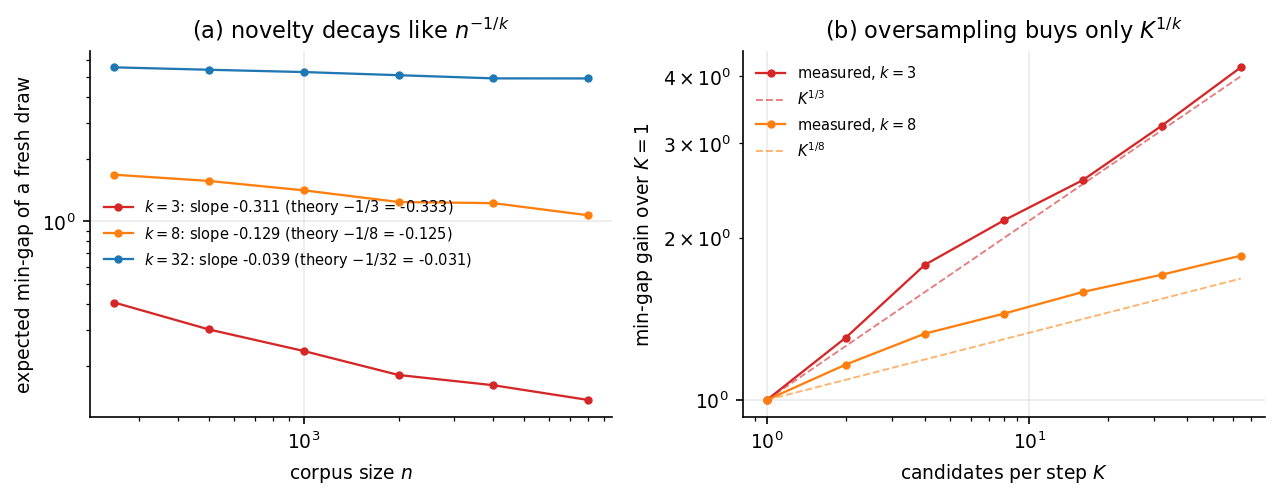
\includegraphics[keepaspectratio,alt={Figure 1. Measured saturation. (a) Expected min-gap of a fresh draw decays as n\^{}(-1/k), with fitted slopes matching theory for k = 3, 8, 32. (b) Best-of-K oversampling buys only K\^{}(1/k).}]{figures/fig5_scaling.png}}

\emph{Figure 1. Measured saturation. (a) Expected min-gap of a fresh
draw decays as n\^{}(-1/k), with fitted slopes matching theory for k =
3, 8, 32. (b) Best-of-K oversampling buys only K\^{}(1/k).}

This is the theorem that makes the axis scoring of §6 possible. It
measures the value of conditioning on a new latent variable as
\textbf{how much of its variation lies outside what the corpus already
spans} --- a computable quantity, in place of the intuition of how
different it sounds.

\subsubsection{5.4 Breadth versus depth}\label{54-breadth-versus-depth}

Given budget \emph{B}, split as \emph{P} prompts × \emph{n} samples
each, with per-prompt switching cost \emph{c} (eliciting a spec,
embedding it, occasionally refining), so \emph{B} = \emph{P}(\emph{c} +
\emph{n}).

\begin{quote}
\textbf{Theorem 4.} With \emph{c} = 0 the coverage-optimal depth is
\emph{n}* = 1. For \emph{c} \textgreater{} 0 the optimum is interior and
increases with \emph{c}.
\end{quote}

Measured: with free switching, depth 1 achieves coverage 0.995 while
spending the entire budget on one prompt achieves 0.091 --- a 10.9×
difference. With \emph{c} = 3, \emph{n}* = 10; with \emph{c} = 30,
\emph{n}* = 30.

\pandocbounded{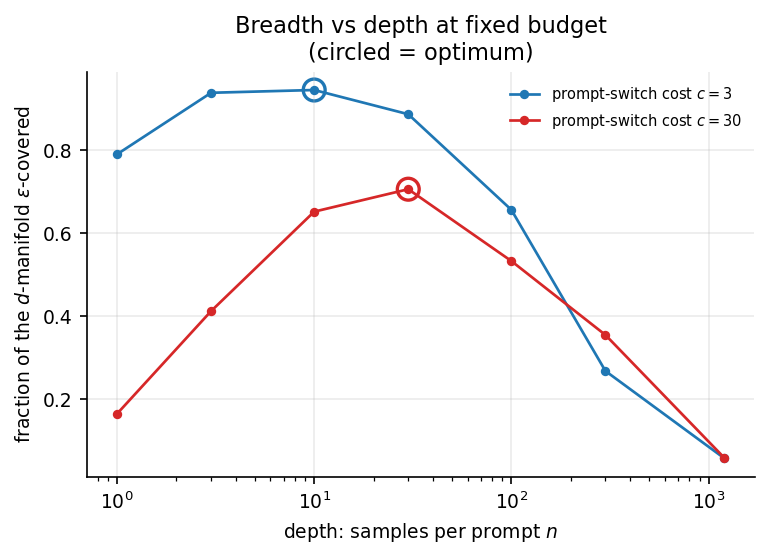
\includegraphics[keepaspectratio,alt={Figure 2. Breadth versus depth at fixed budget. With free prompt-switching the optimum is one sample per prompt; an interior optimum appears only once switching is priced.}]{figures/fig8_breadth_depth.png}}

\emph{Figure 2. Breadth versus depth at fixed budget. With free
prompt-switching the optimum is one sample per prompt; an interior
optimum appears only once switching is priced.}

The engineering reading is that \textbf{the ratio of prompt-switching
cost to sampling cost sets your batch size}, and nothing else does. If
constructing a new spec is as cheap as a generation, generate one item
per spec.

\subsubsection{5.5 What this means for the packing
objective}\label{55-what-this-means-for-the-packing-objective}

Returning to \emph{J}λ: the anchor term is exactly computable from two
running statistics. Writing μ*n* for the corpus centroid,

\[
\frac{1}{n}\sum_i \lVert c - x_i\rVert^2 = \lVert c - \mu_n\rVert^2 + \frac{1}{n}\sum_i \lVert x_i - \mu_n\rVert^2
\]

verified to zero relative error. The second term does not depend on
\emph{c}, so ranking candidates by mean squared distance to the corpus
is ranking by distance to the centroid: \emph{O}(\emph{D}) per
candidate, \emph{O}(1) in \emph{n}. The repulsion term needs a
nearest-neighbour query, which we bound by subsampling. Neither term is
the bottleneck. \textbf{The bottleneck is that both are evaluated on a
candidate set drawn from an \emph{m}-dimensional slice.}

\subsubsection{5.6 The coverage functional is monotone
submodular}\label{56-the-coverage-functional-is-monotone-submodular}

For any measure μ and radius ε, define
\(F(S) = \mu(\bigcup_{x \in S} B(x,\varepsilon))\) on finite S ⊂ R\^{}D.
F is monotone (adding a ball cannot uncover anything) and submodular:
for \(S \subseteq T\) and any \(x\),

F(S ∪ \{x\}) − F(S) ≥ F(T ∪ \{x\}) − F(T).

\emph{Proof sketch.} The marginal gain of \(x\) given \(S\) is
\(\mu(B(x,\varepsilon) \setminus \bigcup_{y \in S} B(y,\varepsilon))\).
Since \(S \subseteq T\) implies
\(\bigcup_S B(y,\varepsilon) \subseteq \bigcup_T B(y,\varepsilon)\), the
set being subtracted only grows, so the gain only shrinks. This is the
standard coverage-function argument; nothing about balls is essential
--- any map from items to measurable "footprints" yields a submodular F.
∎

The same argument applies verbatim to the Monte-Carlo estimator we
actually optimize. Given a reference pool P = \{p\_1, \ldots, p\_P\} of
iid draws from μ,

F̂(S) = (1/P) · \#\{ p ∈ P : dist(p, S) ≤ ε \}

is itself a finite coverage function (item x covers the fixed subset
\(N_\varepsilon(x) = \{p : \lVert p - x\rVert \le \varepsilon\}\) of the
pool, and \(\hat F(S) = |\bigcup_{x \in S} N_\varepsilon(x)|/P\)) so F̂
is monotone submodular exactly, at every sample of the pool. Our
implementation check (§7.13) found 0 violations of either property in
5,000 randomized nested-chain trials, as it must if the code is right.

\subsubsection{5.7 Greedy and its
guarantee}\label{57-greedy-and-its-guarantee}

Because F̂ is monotone submodular with F̂(∅) = 0, the greedy algorithm
that repeatedly adds the item of maximum marginal gain satisfies the
Nemhauser--Wolsey--Fisher bound

\(\hat F(S_{\text{greedy}}) \ge (1 - 1/e) \cdot \max_{|S| \le n} \hat F(S) \approx 0.632 \cdot \mathrm{OPT}\),

and this is tight for the class (maximizing coverage is NP-hard, and
beating 1 − 1/e is hard under standard assumptions, Feige 1998). §5.11
checks the bound against \emph{exact} optima on instances small enough
to enumerate; greedy attained the optimum itself on all ten instances,
comfortably above the bound --- typical behavior, since the 1 − 1/e
worst case requires adversarial structure.

\subsubsection{5.8 Sequential generation is streaming
greedy}\label{58-sequential-generation-is-streaming-greedy}

A generation pipeline cannot pick from a precomputed ground set:
candidates arrive a few at a time (K per step), and must be accepted or
discarded immediately. This is the streaming submodular maximization
regime. Sieve-streaming (Badanidiyuru, Mirzasoleiman, Karbasi, Krause
2014) maintains geometric thresholds and accepts any arrival whose
marginal gain clears one, achieving a (1/2 − δ) guarantee in one pass
with O((k log k)/δ) memory, independent of stream length. Our per-step
rule (take the best of K fresh candidates by marginal gain) is the
natural best-of-K relaxation: weaker in the worst case (an adversarial
stream can starve it) but stronger on exchangeable streams like ours,
where each batch is iid from the current proposal distribution and
thresholding would only discard budget. Empirically the K = 4 stream
rule retains most of full greedy\textquotesingle s value over an
identical ground set (0.484 vs 0.528 covered fraction; §7.14) at a
per-item cost that never touches the whole ground set. What matters for
scaling is that the marginal-gain oracle is O(K · P) per step against a
fixed-size pool with an incrementally maintained covered mask --- O(1)
in n.

\subsubsection{5.9 Estimation error of the Monte-Carlo
coverage}\label{59-estimation-error-of-the-monte-carlo-coverage}

For fixed S, each pool point contributes an iid Bernoulli(F(S))
indicator, so Hoeffding/Chernoff gives

P( \textbar F̂(S) − F(S)\textbar{} \textgreater{} t ) ≤ 2 exp(−2 P t²),

i.e. a 95\% band of t₉₅ = sqrt(ln(2/0.05)/(2P)) --- about ±0.030 at P =
2,000 and ±0.015 at P = 8,000. Two caveats we take seriously. First, the
bound is for fixed S; a set \emph{selected} by optimizing F̂ on the same
pool is biased upward on that pool (the winner\textquotesingle s curse),
which is why every coverage number reported here is computed on held-out
material the selector never saw, and the live pilot reports
selection-pool coverage explicitly labeled as such. Second,
uniform-over-S guarantees would need a union bound over the
(exponentially many) candidate sets; we do not rely on one --- held-out
evaluation makes the fixed-S bound the relevant one. §5.11 confirms the
band empirically: at every pool size tested, ≥ 99\% of 200 independent
pool estimates fell within t₉₅ of a 200k-pool ground truth.

\subsubsection{5.10 Allocation under a known
budget}\label{510-allocation-under-a-known-budget}

Suppose the space decomposes into cells (modes) with measures w\_m, and
within-cell placement is near-saturating: with c\_m items in cell m, the
covered measure of that cell is approximately w\_m · g\_m(c\_m) with
g\_m increasing and concave (each additional exemplar covers a shrinking
uncovered remainder --- submodularity again, now per cell). Maximizing Σ
w\_m g\_m(c\_m) subject to Σ c\_m = n is a concave allocation problem
whose optimum is the water-filling rule: equalize marginal gains w\_m
g\_m′(c\_m) across cells. Three closed-form rules bracket the regimes:

\begin{itemize}
\tightlist
\item
  \textbf{ε large relative to cell diameter} (g\_m saturates after
  \textasciitilde1 item): any rule that puts at least one item per cell
  is near-optimal; equal allocation wastes least; proportional
  over-invests in heavy cells.
\item
  \textbf{ε small} (g\_m near-linear over feasible c\_m, slope ∝
  per-item covered mass ≈ density × ball volume): marginal gain is
  w\_m-weighted throughout, and proportional-to-measure allocation
  dominates equal.
\item
  \textbf{In between}, neither closed form matches water-filling; greedy
  marginal coverage \emph{is} water-filling implemented empirically, and
  wins at the radius it optimizes.
\end{itemize}

The measured allocation experiment (§5.11) shows exactly this pattern,
plus a failure mode the clean theory hides: once greedy has saturated
the pool at its selection radius, its marginal signal is identically
zero and the tie-breaking rule silently decides where the rest of the
budget goes.

\textbf{Depth per condition and switch cost.} The slice theory of §5
sharpens the within-cell side of allocation. For a \emph{fixed}
prompt/spec the generator concentrates on an m-dimensional slice with m
≪ d, so fixed-prompt novelty decays as n\^{}(−1/m) (fitted slopes
−0.472, −0.309, −0.195 for m = 2, 3, 5 --- governed by m, not by the
ambient dimension), and one slice ε-covers a vanishing ε\^{}(d−m)
fraction of the manifold. The budgeted consequence is a breadth-vs-depth
rule whose correct form (their P3, corrected from its first statement)
is: with \emph{free} condition-switching the optimum is the boundary n*
= 1 --- one sample per spec, then move, and an interior optimal depth
exists only once switching carries a real cost c (eliciting a spec,
embedding levels, an occasional refinement call): their measured n*
rises from 1 (c = 0) to 10 (c = 3) to 30 (c = 30). Optimal depth is set
by the switch-cost-to-sample-cost ratio, not by ε alone. Our pipelines
sit near the cheap-switching regime --- in the live pilot we measure c ≈
0.10 generation-equivalents (§7.12: 5 axis-elicitation, refinement and
ledger-mining calls amortized over 50 steps, against 3 generations per
step), which is why every policy here draws its K candidates from K
\emph{fresh} specs rather than sampling any spec deeply. At that switch
cost the sweep puts the optimum at or adjacent to n* = 1, which is what
we do.

\subsubsection{5.11 Numerical
verification}\label{511-numerical-verification}

Each theoretical claim above is checked against a numerical experiment
designed to break it; the underlying numbers are in the accompanying
data release.

\textbf{7.1 Submodularity (exact).} 200 candidates, 5,000-point pool, ε
= 1.0. Over 5,000 random nested chains S ⊂ T with a fresh x: 0
violations of diminishing returns, 0 of monotonicity, worst violation
0.0.

\textbf{7.2 Selection rules head-to-head (no generator).} One shared
ground set of 2,000 candidates, budget k = 300, ε = 1.0, held-out 20k
pool:

{\footnotesize
\begin{longtable}[]{@{}>{\raggedright\arraybackslash}p{\dimexpr 0.5231\linewidth-2\tabcolsep\relax}>{\raggedright\arraybackslash}p{\dimexpr 0.3160\linewidth-2\tabcolsep\relax}>{\raggedright\arraybackslash}p{\dimexpr 0.1609\linewidth-2\tabcolsep\relax}@{}}
\toprule\noalign{}
rule & covered fraction (held-out) & min-gap \\
\midrule\noalign{}
\endhead
\bottomrule\noalign{}
\endlastfoot
full greedy & 0.528 & 0.58 \\
stream greedy, K = 4 & 0.484 & 0.68 \\
random & 0.420 & 0.53 \\
max-min (Gonzalez) & 0.143 & 1.44 \\
\end{longtable}}

Packing is catastrophic \emph{as a coverage algorithm} (below random by
3×), while being unbeatable at its own metric --- the pure-form double
dissociation. Stream greedy with K = 4 keeps 92\% of full
greedy\textquotesingle s coverage.

\textbf{7.3 The (1 − 1/e) bound against exact optima.} Ten instances
with \textbar ground\textbar{} = 30, k = 5 (142,506 subsets enumerated
each): greedy/OPT ratio was 1.0 on every instance; bound 0.632 never
approached.

\textbf{7.4 Monte-Carlo error.} Fixed S of 300 items, ground truth from
a 200,000-point pool (F = 0.4134). Over 200 independent pools per size:
empirical 95th-percentile absolute error 0.042 / 0.020 / 0.011 at P =
500 / 2,000 / 8,000, versus Hoeffding t₉₅ = 0.061 / 0.030 / 0.015; the
fraction of estimates inside the band was 0.99--0.995 ≥ 0.95 everywhere.
P = 20,000 (our estimation pool) implies t₉₅ ≈ 0.0096: pool noise is
well below every effect size we interpret.

\textbf{7.5 Allocation rules.} n = 10,000 across the redteam
world\textquotesingle s M = 60 cells with \emph{known} measures (the
oracle planning question), evaluated against a 50k full-mixture pool:

{\footnotesize
\begin{longtable}[]{@{}>{\raggedright\arraybackslash}p{\dimexpr 0.4072\linewidth-2\tabcolsep\relax}>{\raggedright\arraybackslash}p{\dimexpr 0.1736\linewidth-2\tabcolsep\relax}>{\raggedright\arraybackslash}p{\dimexpr 0.1736\linewidth-2\tabcolsep\relax}>{\raggedright\arraybackslash}p{\dimexpr 0.1228\linewidth-2\tabcolsep\relax}>{\raggedright\arraybackslash}p{\dimexpr 0.1228\linewidth-2\tabcolsep\relax}@{}}
\toprule\noalign{}
rule & ε = 0.6 & ε = 1.0 & ε = 1.6 & ε = 2.4 \\
\midrule\noalign{}
\endhead
\bottomrule\noalign{}
\endlastfoot
equal per cell & 0.046 & 0.494 & 0.9916 & 0.9921 \\
∝ measure & \textbf{0.060} & 0.547 & 0.9917 & 0.9921 \\
∝ sqrt(measure) & 0.055 & 0.531 & 0.9918 & 0.9921 \\
greedy marginal (at ε = 1.0) & 0.004 & \textbf{0.618} & 0.9919 &
0.9921 \\
\end{longtable}}

Three regimes, as §5.10 predicts. At large ε every rule saturates (all ≈
0.992 --- the remaining 0.8\% is junk measure no allocation can reach).
At the greedy-optimized radius, greedy beats the best closed form by 7
points: water-filling in the wild. At small ε, proportional wins among
closed forms (near-linear per-cell returns favor measure-weighting), and
greedy at ε = 1.0 is \emph{terrible} (0.004), for an instructive reason:
greedy saturated its ε = 1.0 pool after roughly half the budget, its
marginal signal went identically to zero, and argmax tie-breaking
silently dumped 5,083 of 10,000 items into one arbitrary cell
(correlation of greedy\textquotesingle s allocation with every closed
form ≤ 0.17). Lesson for practitioners: greedy\textquotesingle s
guarantee says nothing about what it does \emph{after} it has won; at a
finite budget you must either select at the smallest ε you care about,
or hand the post-saturation residual to an explicit rule (e.g.
proportional), or lower ε adaptively as gains vanish.

\textbf{7.6 The reachability gap (Proposition 1, measured).} Identical
greedy selection (ε = 1.0, k = 300, \textbar ground\textbar{} = 2,000),
three proposal distributions, one held-out full-mixture pool. An
\emph{oracle} ground set drawn from the full latent mixture (the best a
selector could do if conditioning could reach everything) covers 0.387.
A \emph{proposal-limited} ground set drawn from the base specs (which
reach 25 of 60 modes) covers 0.212: a reachability gap of 17.4 points
that no selection algorithm can close, because the deficit is in what
the generator can be made to emit, not in how candidates are chosen. A
\emph{refined-proposal} ground set (one spec per mode --- the target
recursive refinement works toward) covers 0.374, recovering 92.5\% of
the gap. This is Proposition 1 made quantitative: the (1 − 1/e)
guarantee binds relative to the proposal support, and conditioning (not
selection) is where the missing coverage lives.

\textbf{Lattice size is not reachable dimension.} Using the
slice-structured world, in which specs compose level directions
additively, we build two worlds with \emph{identical} lattice size
L\^{}A = 1,024 distinct specs but different rank of the level-direction
span: full-rank (rank 10, reachable dimension 13) versus low-rank (all
axes forced into a shared 2-dim subspace: rank 2, reachable dimension
5). Same budget (n = 2,000 random-spec draws), same radius (ε = 0.27):
the low-rank world\textquotesingle s own reachable pool is 68.1\%
covered where the full-rank world\textquotesingle s is 49.0\%. The
number of distinct prompts you can write says nothing about how much
there is to cover; covered volume is governed by reachable dimension,
and a huge lattice over low-rank level directions is a thin space
wearing a combinatorial costume. For coverage this distinction is
sharper than for packing, because the denominator itself is set by
reachable dimension.

\textbf{Refinement direction: density versus reach.} The earlier result
--- naive refinement hurt, because tight children near saturated parents
concentrate mass where the corpus already sits --- ports to coverage,
with a measurement subtlety worth recording. Nearest-neighbor distance
cannot distinguish density-refinement from reach-refinement: child draws
sit ≈ 1.04 from the nearest corpus point whether they moved in-span or
off-span, because a 1,500-item corpus is sparse in its own
13-dimensional occupied span. Density-versus-reach is a \emph{span}
property, and must be measured with span-level metrics: \emph{local}
children (tight, 0.25× displacement --- the naive move) produce draws of
which 36.7\% are already covered by the pre-refinement corpus at the
coverage radius, and add +0.02 effective dimensions --- almost pure
density. Full-length \emph{isotropic} displacement produces 0\%
pre-covered draws and +0.13 effective dimensions;
\emph{transversality-guided} displacement 0\% and +0.14, with off-span
displacement energy 0.915 vs 0.823 unguided. The honest reading: (i) the
damning comparison is local-vs-far, and "split the saturated cell into
tighter sub-levels" is only worth its cost if the children actually
move; (ii) guidance beats unguided displacement, but by little
\emph{here}, because this corpus occupies only a thin span (6 of 64
dimensions at the 95\% energy level), and a random direction is already
82\% transverse to it --- guidance matters most when the corpus has
already spread, which is exactly the late-run regime where refinement
fires.

\subsection{6. Method: Recursive Axis
Conditioning}\label{6-method-recursive-axis-conditioning}

The loop below is written once and pointed at a measure. We call it
\textbf{Recursive Axis Conditioning} (RAC): the generator is asked for
the language-valued axes along which its own outputs can differ, those
axes are ranked and their most-different levels chosen, and an axis that
runs out of transverse variation is split into finer conditional
sub-axes. Two components read the measure and the rest do not, which is
what makes the same stack serve objectives whose optima conflict. The
recursion is what the name refers to, and it is the part that changes
the asymptote rather than the constant.

\pandocbounded{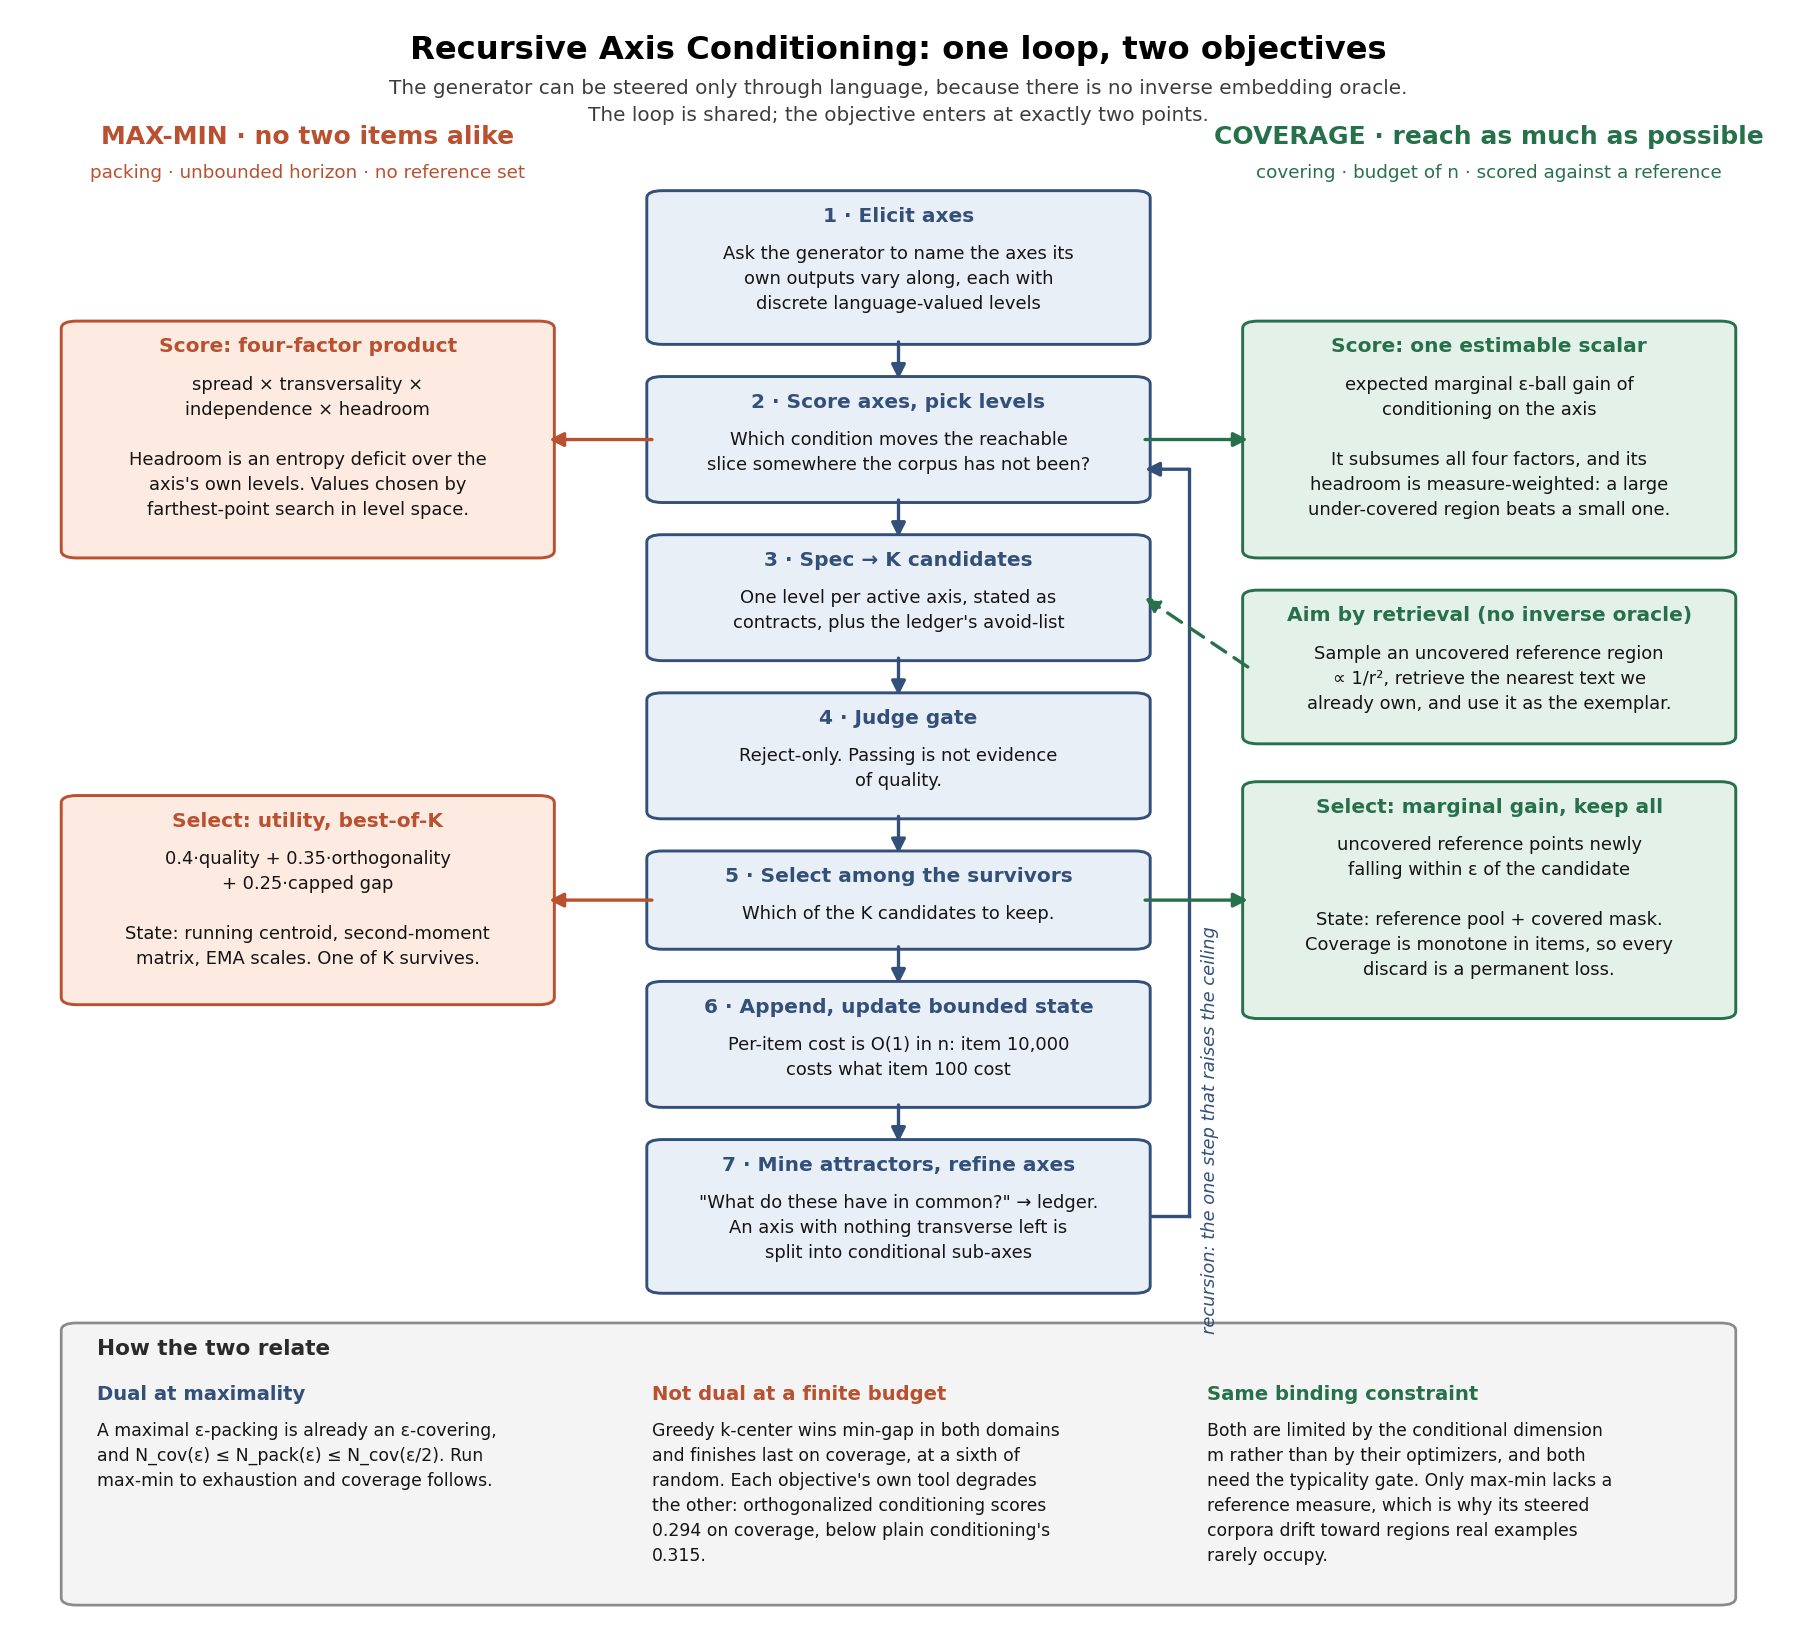
\includegraphics[keepaspectratio,alt={Figure 3. Recursive Axis Conditioning. Steps 1--7 are shared whatever the measure. The measure enters at two points only: how a candidate axis is scored (step 2) and how one of the K candidates is chosen (step 5). Everything else --- elicitation, the contracts, the reject-only gate, the attractor ledger, the refinement trigger --- is the same machinery. Coverage adds one step max-min has no use for, since only coverage has a reference distribution to aim at.}]{figures/fig15_rac_diagram.png}}

\emph{Figure 3. Recursive Axis Conditioning. Steps 1--7 are shared
whatever the measure. The measure enters at two points only: how a
candidate axis is scored (step 2) and how one of the K candidates is
chosen (step 5). Everything else --- elicitation, the contracts, the
reject-only gate, the attractor ledger, the refinement trigger --- is
the same machinery. Coverage adds one step max-min has no use for, since
only coverage has a reference distribution to aim at.}

Reading the diagram: the seven boxes down the centre run once per
accepted item, and each carries its own colour so the text below can
name it.

The \textbf{violet} \emph{Elicit axes} step happens before any item is
generated. The generator is asked to name the dimensions along which its
own outputs in this domain could differ, each with a small set of
discrete, language-valued levels. For instrumental music it returned
\emph{formal trajectory}, \emph{timbral centre of gravity}, \emph{pulse
relationship} and four others; for poetry, \emph{temporal stance} and
\emph{the register the poem refuses}. These names are the entire
steering vocabulary, because they are the only thing that can be written
into a prompt.

The \textbf{blue} \emph{Score axes, pick levels} step is the first of
the two places the objective enters, and the arrows leaving it left and
right are the fork. It answers which of the available axes to condition
on next and which of that axis\textquotesingle s levels to use. The
\textbf{teal} \emph{Spec → K candidates} step turns the chosen levels
into one specification, states them to the generator as contracts the
text must satisfy rather than as suggestions, attaches the current
avoid-list, and draws K completions. The \textbf{amber} \emph{Judge
gate} scores each candidate in a separate call and rejects those below
the bar. The gate can only reject: a candidate that passes has not been
endorsed, and nothing downstream treats passing as evidence of quality.

The \textbf{crimson} \emph{Select among the survivors} step is the
second place the objective enters, and the second fork. The
\textbf{grey} \emph{Append, update bounded state} step commits the
winner and rolls the running statistics forward; every piece of state it
touches is fixed-size, which is what makes the ten-thousandth item cost
what the hundredth cost. The \textbf{magenta} \emph{Mine attractors,
refine axes} step closes the loop. Every twenty-five accepts it shows
the model a sample of the corpus and asks what those items have in
common, appending the answer to the ledger that becomes the next
prompts\textquotesingle{} avoid-list. When the scoring step reports that
no available axis has anything transverse left to offer, this step
splits the exhausted axis into finer sub-axes that apply only inside the
region that exhausted it, and the arrow running back up to the blue step
is that recursion.

The \textbf{orange} boxes on the left and the \textbf{green} boxes on
the right are the only differences between the two objectives. At the
scoring fork, max-min multiplies four measurable factors and chooses
each axis\textquotesingle s most-different levels by farthest-point
search in level space, while coverage replaces the product with the
expected marginal ε-ball gain of conditioning on that axis, a single
quantity that already contains all four and whose headroom term is
weighted by measure rather than by counts. At the selection fork,
max-min keeps one of the K by a weighted utility and carries a running
centroid and second-moment matrix, while coverage keeps the candidate
that newly covers the most reference points and carries a reference pool
with an incremental covered mask. Coverage keeps every candidate that
clears the gate, since covered measure only grows with items and a
discard cannot be undone.

The green box with no orange counterpart is \emph{Aim by retrieval}.
Coverage is scored against a reference distribution, so it can pick a
specific under-covered region to attack, sampling one in proportion to
how sparse it is. Having no inverse oracle, it cannot turn that target
point into text; instead it retrieves the nearest text it already owns
and hands that to the generator as the exemplar to move away from or
toward. Max-min has no such box because it has no reference distribution
to aim at, which is the same absence that lets its steered image corpora
settle into regions real artworks rarely occupy.

The grey band along the bottom is the relationship between the two
columns, and it is not a single answer. Run max-min to exhaustion and
coverage comes free, because a maximal ε-packing is already an
ε-covering. Stop at a finite budget and the two come apart far enough
that each objective\textquotesingle s characteristic tool damages the
other\textquotesingle s score.

\subsubsection{6.1 The stack}\label{61-the-stack}

Per accepted item, a bounded number of model calls regardless of corpus
size:

\begin{enumerate}
\def\labelenumi{\arabic{enumi}.}
\tightlist
\item
  \textbf{Spec choice.} Sample a pool of specs from the current axis
  lattice; embed their descriptions; keep the one with the largest
  residual outside the corpus\textquotesingle s occupied eigenspace.
  Orthogonalization at the level of \emph{conditions}, not outputs.
\item
  \textbf{Generation.} \emph{K} parallel completions conditioned on the
  spec, with the spec\textquotesingle s levels stated as
  \textbf{contracts} (behaviors the text must exhibit, not suggestions),
  plus an explicit avoid-list from the ledger.
\item
  \textbf{Judging.} One separate call scores craft (or, for exam items,
  validity), and checks each required behavior. Generation never grades
  itself.
\item
  \textbf{Selection.} Utility = 0.4·quality + 0.35·orthogonality +
  0.25·capped gap, behind a typicality gate: a hard rejection of
  candidates lying beyond \emph{z} running radii from the corpus
  centroid. The gate is negative supervision only (it may reject, never
  endorse, and passing it is not evidence of quality), and the gap term
  is \textbf{capped} at 2 running scales, so no candidate earns
  unbounded credit for sitting far from everything.
\item
  \textbf{Mining.} Every 25 accepts, show the model 50 sampled items and
  ask what they have in common. Append the answer to a JSONL ledger; a
  bounded slice becomes the next prompts\textquotesingle{} avoid-list.
\item
  \textbf{Refinement.} On a saturation signal, ask the generator to
  split the dominant saturated cell.
\end{enumerate}

Every state the policy reads is bounded: running centroid and
second-moment, EMA scales, a fixed ledger slice, a recent window plus a
bounded random subsample of older items. The marginal cost of item
10,000 equals that of item 100.

\subsubsection{6.2 Scoring candidate
axes}\label{62-scoring-candidate-axes}

Theorem 3 says progress requires moving the prompt transversely to what
the corpus already spans. Theorem 4 says move often. Together they pose
a concrete question at every step: \textbf{among the latent variables we
could condition on next, which one moves the slice most transversely,
per unit of budget?} Since we have no inverse oracle, this is the
closest available substitute for computing the ideal next item.

Each candidate axis \emph{a} has language-valued levels
\emph{L}(\emph{a}). We embed the level descriptions and read off four
quantities.

\subsubsection{6.3 The four factors}\label{63-the-four-factors}

\textbf{Spread} --- mean pairwise distance between
\emph{a}\textquotesingle s level embeddings. Are this
axis\textquotesingle s values actually different \emph{from each other}?
An axis whose levels are near-synonyms cannot separate outputs however
it is sampled. This catches the most common failure of LLM-proposed
axes: plausible-sounding dimensions whose levels all mean the same
thing.

\textbf{Transversality} --- the fraction of \emph{a}\textquotesingle s
level-to-level variation lying outside the corpus\textquotesingle s
occupied eigenspace (top eigenvectors of the second-moment matrix
carrying 80\% of spectral energy). This is Theorem 3 made into a number.
An axis whose levels differ only along directions the corpus already
spans adds density, not reach.

\textbf{Independence} --- 1 − max principal-angle cosine between
\emph{a}\textquotesingle s variation subspace and those of the axes
\textbf{already in use}. An axis that restates an active axis is
redundant however transverse it looks alone. Independence is measured
against the active set and never against rival candidates: two equally
good candidates would otherwise drive each other\textquotesingle s score
to zero and rank below a useless axis with no near-twin. Redundancy
\emph{among} candidates is a selection problem, handled by greedy
selection that re-scores after every pick, so a duplicate is penalized
at the point where the redundancy comes into existence.

\textbf{Headroom} --- a normalized entropy deficit of how unevenly the
corpus has sampled \emph{a}\textquotesingle s levels, plus the fraction
of levels never used. This is the only time-varying factor; it is what
makes the ranking change as generation proceeds rather than being a
fixed property of the axis set. An axis can be excellent and already
spent.

The \textbf{promise} of an axis is the product:

\[
\mathrm{promise}(a) = \mathrm{spread}(a)\cdot\mathrm{transversality}(a)\cdot\mathrm{independence}(a)\cdot\mathrm{headroom}(a)
\]

Multiplicative, not additive, and deliberately so: an axis needs all
four, and any one at zero should zero the score rather than be averaged
away by the others. A high-spread axis with zero transversality is a
distinction without a difference; a perfect axis with zero headroom is
already spent.

\subsubsection{6.4 Choosing values, and
recursing}\label{64-choosing-values-and-recursing}

Once an axis is chosen we do not sample its levels uniformly. We take
the \textbf{max--min subset} of its level embeddings by greedy
farthest-point search, seeded deterministically at the level furthest
from the level centroid --- the packing problem again, one level down.

When the best available promise falls below a floor, the axis scoring
emits \texttt{decision:\ "refine"} instead of \texttt{"condition"}. This
is the \textbf{exhaustion signal}, and it is the honest one: it says the
current lattice has nothing transverse left to offer, and no amount of
further sampling will change that. The system then asks the generator to
split the exhausted level into finer sub-levels (§6.5), producing a
child axis scored by this same axis scoring. On the ground-truth test
with only in-span axes available, the axis scoring correctly returns
\texttt{refine}.

Cost is \emph{O}(\textbar{}\emph{A}\textbar{} · \emph{D}²) per decision
and does not grow with \emph{n}.

\subsubsection{6.5 Eliciting and refining latent
behaviors}\label{65-eliciting-and-refining-latent-behaviors}

We ask the generator for axes that are near-orthogonal, structural
rather than topical, and whose levels are all usable --- explicitly
steering away from subject matter, length, and rhyme toward craft
decisions. On the live run this produced axes including \emph{temporal
stance}, \emph{relationship to its own claim}, \emph{syntactic weather},
and \emph{the register the poem refuses}.

Refinement shows the model the saturated cell and the mined attractors
and asks it either to split a level into finer sub-levels or to mint a
new axis that applies only inside that cell. Refinement axes are
\textbf{conditional} (they apply only when their parent level was
chosen), so the lattice is a tree, and refining a saturated region does
not inflate cost elsewhere.

\subsubsection{6.6 The covering
instantiation}\label{66-the-covering-instantiation}

The covering instantiation is the same RAC stack with the selection
objective and its bookkeeping swapped from packing to covering; we write
RAC-coverage for it and RAC-packing for the objective of the preceding
sections. Figure 3 draws the shared loop and marks the two points where
the objective enters it: how a candidate axis is scored, and how one of
the K candidates is chosen. Coverage adds a third element that packing
has no use for, described below, because only coverage has a reference
distribution to aim at. Concretely:

\textbf{Reachable pool (the denominator).} Before selection begins, draw
a pool of cheap, unconditioned samples from the generator and embed
them. This pool \emph{is} the Monte-Carlo measure: coverage means
coverage of it. Live, the pool is 240 one-shot prompts. Cost is O(P)
once, amortized over the whole run.

\textbf{Elicited axes and specs.} The generator is asked (before
generating any items) to name the latent axes along which items in this
domain can differ, each with discrete language-valued levels (live: 6
axes for evaluation prompts, e.g. persona pressure, trap construction,
response obligation). A spec is one level per applicable axis; K specs
are sampled per step and one candidate is generated under each. Axes
give the proposal distribution spread the base generator lacks; they are
the reason the method\textquotesingle s candidates are worth ranking at
all.

\textbf{Score-guided conditioning (the coverage adaptation).} The
generation axis scoring of §6.3 ranks candidate axes by a four-factor
product --- spread (are the axis\textquotesingle s levels different from
each other), transversality (does their variation point outside the
corpus\textquotesingle s occupied eigenspace), independence (measured
against axes already in use, never against rival candidates --- scoring
candidates against each other makes duplicates zero each other out), and
headroom (an entropy deficit over the axis\textquotesingle s sampled
levels). Under a \emph{coverage} objective this product collapses, and
the collapse is itself a packing-vs-covering result. Packing has no
per-axis marginal decomposition (min-gap is a global property), so the
axis scoring must approximate "will this axis move the slice somewhere
new" from four separate geometric proxies. Submodular coverage has an
exact marginal quantity: the \textbf{expected marginal ε-ball gain of
conditioning on the axis},
\(\mathbb{E}_{x \sim a}[F(S \cup \{x\}) - F(S)]\). That one scalar
subsumes the four factors: an axis with near-synonym levels (no spread)
or whose slices sit inside covered territory (no transversality) or
which duplicates an axis already exploited (no independence, because the
covered mask already contains that axis\textquotesingle s contribution
and re-scores every candidate after every accept --- the same greedy
re-scoring the axis scoring performs by hand, executed here by the
objective itself) or whose region is already covered (no headroom) all
have small expected marginal gain, and the headroom that remains is
\emph{measure-weighted} by construction --- a large under-sampled region
beats a small one because it holds more uncovered pool mass. We keep the
embedding-based spread and transversality (level-description embeddings
against the accepted corpus\textquotesingle s occupied eigenspace), and
replace its entropy headroom with the measure-weighted estimate
(per-level mean observed marginal gain, optimistic for unused levels);
the top-two axes by this promise become the step\textquotesingle s
dominant design pressures, with their most-different levels chosen by
farthest-point selection in level-embedding space --- the axis scoring
acting as the surrogate inverse of Proposition 2.

\textbf{Coverage-greedy selection.} Each step: embed the K candidates,
compute each one\textquotesingle s marginal gain --- the number of
not-yet-covered pool points within ε\_sel, and accept the gated
candidate of maximum gain (ties broken by judge score). The covered mask
is updated incrementally; per-step cost is O(K · P + P) regardless of n.

\textbf{Judge gate (quality/typicality).} A separate LLM call
(generation never self-grades) scores each candidate on a rubric;
candidates below the bar are ineligible regardless of gain. The gate is
negative supervision only: if every candidate fails, the step falls back
to best-judged rather than emitting nothing, and the rejection is
logged.

\textbf{Attractor ledger.} Every 20 accepted items (50 under the packing
objective), the accepted corpus is shown to the model with the question
"what do these have in common?"; the mined attractors are appended to a
JSONL ledger, and a bounded top-K slice becomes explicit negative
constraints in subsequent generation prompts. The ledger is append-only;
its influence on any single prompt is fixed-size.

\textbf{Recursive refinement + pool refresh.} When recent accepted
items\textquotesingle{} marginal gains saturate (the
region\textquotesingle s balls mostly re-cover covered ground), the
responsible region of spec-space is described back to the generator,
which either splits an axis level into finer sub-levels or mints a new
axis that applies inside that cell --- conditional axes forming a tree,
as above. The budgeted setting adds one obligation the infinite-horizon
setting does not have: refinement changes the reachable distribution, so
the reference pool must be refreshed with draws from the newly opened
region, or the selector will see zero gain precisely where the new
territory is: its balls cover no \emph{old} pool points.

\subsubsection{6.7 Why "orthogonalize", not
"randomize"}\label{67-why-orthogonalize-not-randomize}

Forcing randomness (raising temperature, injecting random seed words)
buys variance in the surface while leaving the mode structure intact,
and degrades quality monotonically because temperature cannot
distinguish \emph{surprising} from \emph{wrong}. The measurements bear
this out: raising the sampling temperature to 1.6 moves distinct-2 from
0.3341 to 0.3342 and leaves 71.0\% of the corpus byte-identical
duplicates, against 73.6\% at the default setting.

Forcing approximate orthogonality asks a different question (which
direction is this corpus not yet spending energy on), which has a
computable answer, improves rather than degrades quality when paired
with a quality term, and stays informative as \emph{n} grows. "Be
random" gets no harder to satisfy and no more useful.

\subsection{7. Experiments}\label{7-experiments}

Every number below states the measure it is computed under and the
\emph{n} it is computed at, since §4.1 showed how far the measures can
diverge on one corpus. Generator: \texttt{openai/gpt-5.6-luna} via
OpenRouter. Text embeddings: \texttt{nomic-embed-text} (768-d) served
locally by Ollama, so embedding is free and the loop is never
rate-limited by its own measuring instrument. Images:
\texttt{gpt-image-1-mini}. Image embeddings: CLIP ViT-B/32. Audio: Lyria
3 Pro instrumentals. Audio embeddings: CLAP and MERT. Every corpus is
append-only JSONL with embeddings checkpointed alongside, resumable
after a kill.

\subsubsection{7.1 What we measure, and what each measure
misses}\label{71-what-we-measure-and-what-each-measure-misses}

Every number below is one of the following. We report several because
they disagree, and a corpus that one of them calls healthy another calls
collapsed.

\textbf{Exact-duplicate rate.} The fraction of the corpus that is
byte-identical to something else in it. Unambiguous, cheap, and the
first thing to compute: a naively prompted psychometric corpus is 73.6\%
duplicates, and no embedding, threshold or interpretation is needed to
see it. It is also blind to paraphrase. Deduplicating that corpus
removes 2,726 identical copies of one question and leaves behind the
same question with one word changed, the same question with its options
reshuffled, and the same question on different numbers.

\textbf{Distinct-\emph{n}, self-repetition, \emph{n}-gram Vendi.}
Surface statistics over token sequences. They catch templating that
duplicate rate misses and they read meaning not at all. A poetry corpus
with a 0.000 duplicate rate and a distinct-2 of 0.610 --- healthy by
both --- has eight of eight sampled poems opening \emph{At dusk/dawn,
the windows/river/rooftops gather \ldots{}}.

\textbf{Mean-centered embedding Vendi.} The exponential of the von
Neumann entropy of the corpus Gram matrix, an effective number of
distinct items. It summarises the whole spectrum, which makes it
insensitive to local structure: on the poetry pair above it reads 37.00
for the templated corpus and 38.81 for the varied one, a difference the
page makes in a second. Centering matters as much as the statistic ---
the shared mean direction of text embeddings compresses the uncentered
score by roughly 2.7×, so an uncentered Vendi is reporting the cone as
much as the content.

\textbf{Median nearest-neighbour distance.} How much room the typical
item has. It registers the poetry difference the Vendi Score misses,
0.089 against 0.239, and it is the statistic that goes to exactly zero
when the median item has a perfect twin. It says nothing about the shape
of the corpus as a whole.

\textbf{Worst-case nearest-neighbour distance (the packing radius).} The
minimum over all pairs. It is the only measure here under which a single
collision is a defect regardless of everything else, which is what an
exam bank needs: two items testing the same rule are a security failure
whatever the other 2,498 items look like. Optimizing it is the max-min
objective of §4.2.

\textbf{Coverage, density, precision and recall against a reference.}
Ratios computed against a corpus of real examples, using reference-side
k-NN radii so nothing is tunable per corpus. These are the only measures
here that know what the space is supposed to look like, and the only
ones that let corpora of different scales be compared, which is why the
head-to-head against released corpora uses them. Covered fraction at a
\emph{fixed} radius does not survive that comparison: it correlates
−0.991 with within-corpus spacing, so it ranks corpora by how tightly
they cluster rather than by how much they reach.

\textbf{A judged threshold.} Where an application defines the failure,
the radius can be measured instead of assumed. Adjudicating 236 item
pairs blind puts the enemy-item radius for exam questions at δ = 0.0354
on this embedder, and that number, rather than a convention, is what a
usable-capacity table rests on.

\textbf{Measures on the rendered artifact.} When the text is an
instruction to a second generative model, the corpus that matters is the
rendered one. Text embeddings predict rendered-image similarity at
\emph{r} = 0.170, so a text-side measure explains about 3\% of the
variance in what the reader receives, and every text-side method in this
literature, ours included, is optimizing a proxy.

Two lessons run through the rest of the paper. The measure has to be
named for a diversity claim to carry information, and it has to be
computed at the level of the artifact being shipped.

\subsubsection{7.2 Domains}\label{72-domains}

\textbf{DALL·E instructions for post-modern artworks.} Diversity
\emph{is} the product: a clustered instruction set renders to a
clustered image set. Chosen also because it lets us measure the same
corpus in three spaces --- words, text-embedding, and the rendered
picture.

\textbf{Psychometric test questions.} Multiple-choice items assessing
general reasoning. Two items with the same construct and the same
surface are redundant at best and, in an operational bank, a validity
problem.

\textbf{Instrumental-music prompts.} The longest chain in the paper:
latent axes → a text prompt → a two-minute instrumental → an audio
embedding. We render with Lyria 3 Pro (\texttt{lyria-3-pro-preview}),
which returns roughly two minutes of audio per call in about 20 seconds
and emits its own section plan
(\texttt{{[}{[}A0{]}{]}\ {[}{[}B1{]}{]}\ {[}{[}C2{]}{]}\ {[}{[}D3{]}{]}}),
a model-reported description of the form it chose that gives a discrete
structural signal without waveform analysis. The generator proposed
seven compositional axes for this domain --- \emph{formal trajectory},
\emph{inter-layer rhythmic relationship}, \emph{harmonic motion},
\emph{timbral centre of gravity}, \emph{density contour}, \emph{pulse
relationship}, \emph{opening and closing frame} --- craft decisions
rather than genre labels, each expressible as something audible.

\textbf{Poetry.} A smaller pilot corpus, used to elicit and inspect the
axis machinery on a domain where craft rather than content carries the
variation, and to illustrate what the attractor mining recovers (§7.16).

\textbf{Prompt length.} A text-to-music model honours concrete,
performable direction (named instruments, room character, register,
articulation, rhythmic feel, how it ends), and ignores paragraphs of
abstract compositional theory. Long prompts therefore inflate every
text-side diversity metric while changing the audio far less, which is
the proxy gap §7.15 measures. Prompts are held to 2--4 sentences
(\textasciitilde300 characters target, 423--449 mean in the corpora
below) of specifically audible, instrumental-only direction, and the
audio metrics decide.

\subsubsection{7.3 Methods compared}\label{73-methods-compared}

Five of these are real published approaches, implemented faithfully
rather than as strawmen, each getting the same generator, the same
embedder, and the same budget accounting as ours.

{\footnotesize
\begin{longtable}[]{@{}>{\raggedright\arraybackslash}p{\dimexpr 0.4002\linewidth-2\tabcolsep\relax}>{\raggedright\arraybackslash}p{\dimexpr 0.5998\linewidth-2\tabcolsep\relax}@{}}
\toprule\noalign{}
arm & what it is \\
\midrule\noalign{}
\endhead
\bottomrule\noalign{}
\endlastfoot
\texttt{naive} & plain repeated prompting --- the honest floor \\
\texttt{high\_temp} & temperature 1.6 --- the trivial diversity lever \\
\texttt{self\_instruct} & \textbf{Self-Instruct / Alpaca}: few-shot
exemplars sampled from the pool, plus ROUGE-L ≤ 0.7 rejection against
it \\
\texttt{evol\_instruct} & \textbf{Evol-Instruct (WizardLM)}: sample an
existing item, apply a random evolution operator (deepen, concretize,
add constraint, harder reasoning, mutate form) \\
\texttt{persona} & \textbf{Persona-Hub / AttrPrompt}: a flat catalogue
of personas × attributes, sampled uniformly \\
\texttt{rac} & \textbf{Recursive Axis Conditioning} (ours): recursively
elicited axes, spec-level orthogonalization, capped repulsion behind a
typicality gate, append-only attractor ledger \\
\texttt{rac+vision} & RAC, plus steering on the \emph{rendered image}
(§7.15) \\
\end{longtable}}

\texttt{persona} is the load-bearing comparison. It has language-valued
latent conditioning (the same basic idea as ours), but no orthogonality
selection, no ledger, and no recursive refinement. The gap between
\texttt{persona} and \texttt{rac} isolates exactly what those three
components buy.

One faithfulness caveat we chose deliberately:
Self-Instruct\textquotesingle s ROUGE filter compares a candidate
against the entire pool, which is O(\emph{n}) longest-common-subsequence
computations per candidate and comes to dominate the loop at \emph{n} in
the thousands. We compare against a bounded random sample of 120 pool
members. This makes our reimplementation \emph{weaker} than the original
at large \emph{n}, and that is itself the point: the
original\textquotesingle s redundancy check does not have an infinite
horizon, because its cost grows linearly in the corpus it is protecting.

\subsubsection{7.4 Duplication under repeated
sampling}\label{74-duplication-under-repeated-sampling}

Two 10,000-item corpora, one call each, no selection:

{\footnotesize
\begin{longtable}[]{@{}>{\raggedright\arraybackslash}p{\dimexpr 0.3763\linewidth-2\tabcolsep\relax}>{\raggedright\arraybackslash}p{\dimexpr 0.1175\linewidth-2\tabcolsep\relax}>{\raggedright\arraybackslash}p{\dimexpr 0.1440\linewidth-2\tabcolsep\relax}>{\raggedright\arraybackslash}p{\dimexpr 0.1859\linewidth-2\tabcolsep\relax}>{\raggedright\arraybackslash}p{\dimexpr 0.1763\linewidth-2\tabcolsep\relax}@{}}
\toprule\noalign{}
domain & \emph{n} & unique texts & exact-duplicate rate & most-repeated
item \\
\midrule\noalign{}
\endhead
\bottomrule\noalign{}
\endlastfoot
DALL·E instructions & 10,000 & 10,000 & 0.000 & 1× \\
psychometric items & 10,000 & 2,645 & \textbf{0.736} &
\textbf{2,726×} \\
\end{longtable}}

In the psychometric domain, 73.6\% of a ten-thousand-item corpus is
exact duplicate text, and a single question accounts for 2,726 of them.
The four most frequent items are these:

{\footnotesize
\begin{longtable}[]{@{}>{\raggedright\arraybackslash}p{\dimexpr 0.4544\linewidth-2\tabcolsep\relax}>{\raggedright\arraybackslash}p{\dimexpr 0.5456\linewidth-2\tabcolsep\relax}@{}}
\toprule\noalign{}
copies & item \\
\midrule\noalign{}
\endhead
\bottomrule\noalign{}
\endlastfoot
2,726 & What number comes next in the sequence: 2, 6, 12, 20, 30, ? (A.
40 B. 42 C. 44 D. 46) \\
655 & What number \emph{should} come next in the sequence: 2, 6, 12, 20,
30, ? (A. 40 B. 42 C. 44 D. 46) \\
467 & What number comes next in the sequence: 2, 6, 12, 20, 30, ? (A. 36
B. 40 C. 42 D. 44) \\
434 & What number comes next in the sequence: 3, 8, 15, 24, 35, ? (A. 46
B. 48 C. 50 D. 52) \\
\end{longtable}}

Deduplication does not rescue this corpus. Removing the 2,726 identical
copies leaves the three paraphrases behind, and a paraphrase of a live
item is an enemy item on any bank a psychometrician would sign off on.
No embedding, no threshold, and no interpretation is required to see
this; it is byte-identical repetition, and it is what a strong
instruction-tuned model does when asked the same reasonable question ten
thousand times.

Temperature barely helps: at \emph{T} = 1.6 the duplicate rate is still
0.710. Conditioning nearly eliminates it: persona conditioning drops it
to 0.009, and axis conditioning to 0.000. Between those two numbers ---
randomness does not buy diversity, conditioning does.

It also shows the failure is domain-shaped and invisible from one
vantage point. The identical pipeline, prompt style, and model produce
zero duplicates on DALL·E instructions. A practitioner who validated
their pipeline on the first domain and deployed it on the second would
ship a bank that is three-quarters one question.

\pandocbounded{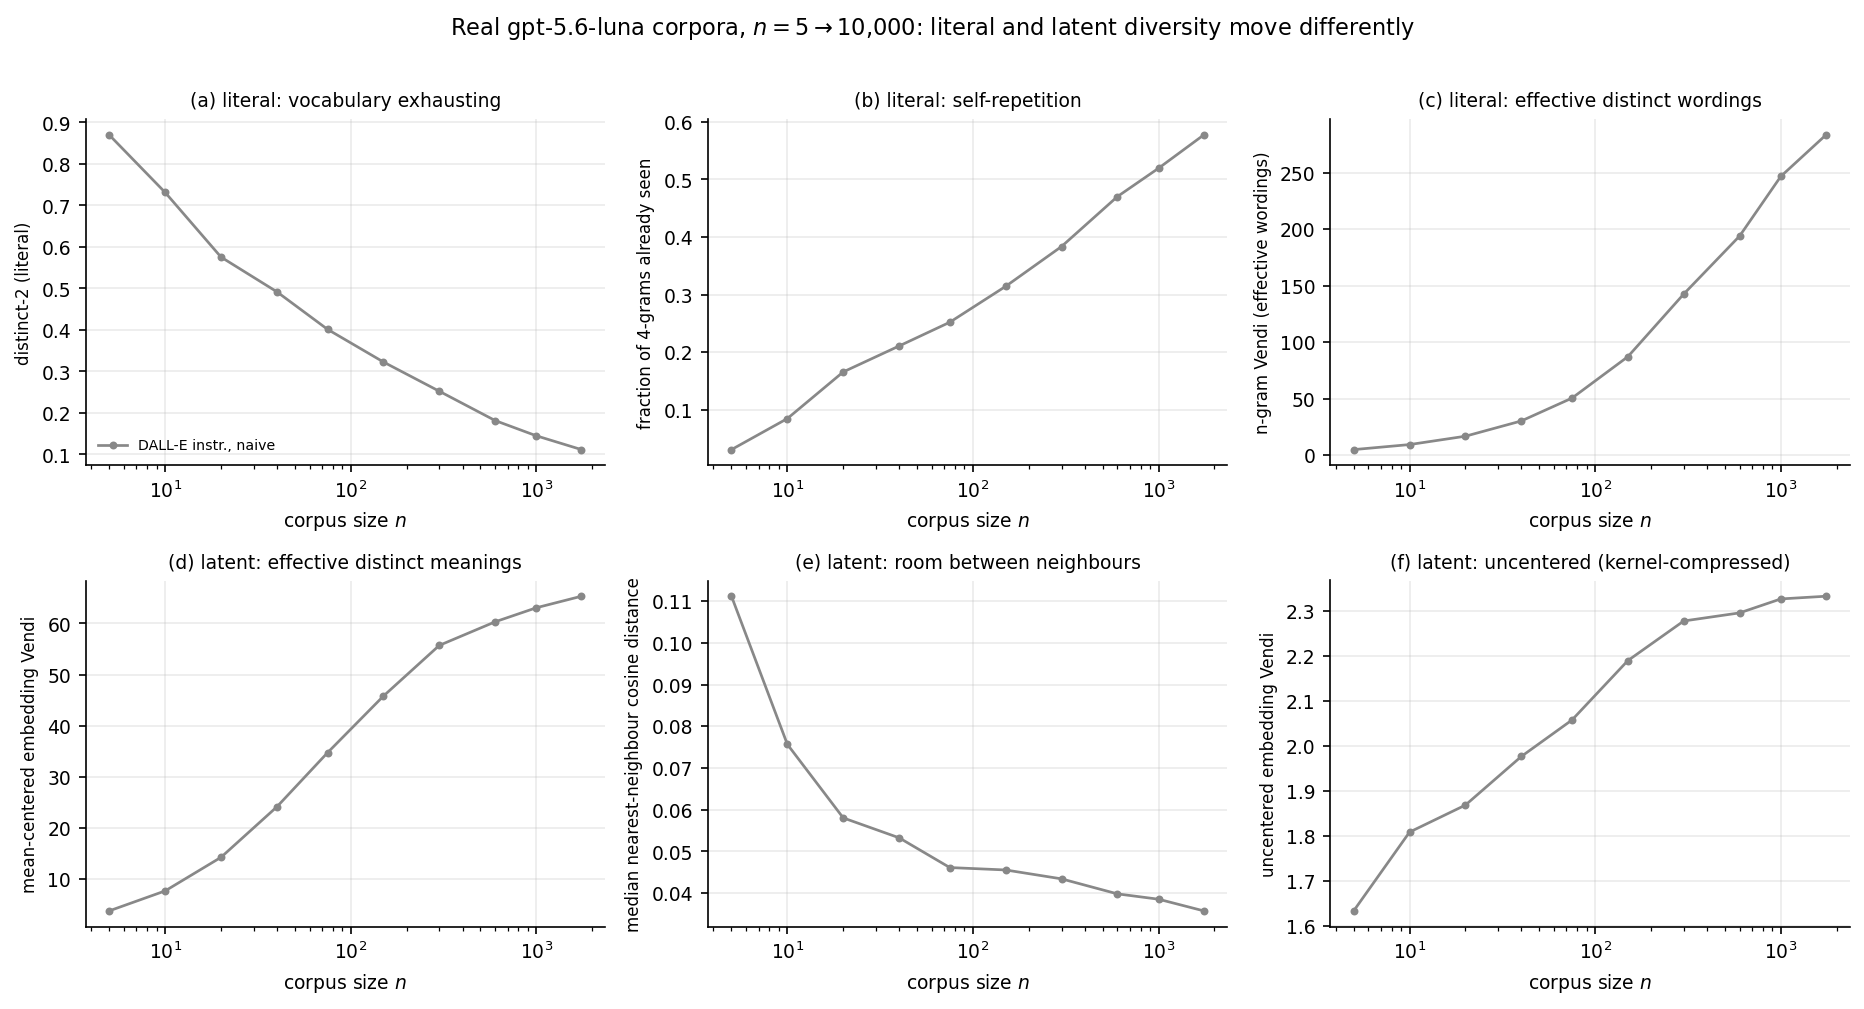
\includegraphics[keepaspectratio,alt={Figure 4. Real gpt-5.6-luna corpora, n = 5 to 10,000. Literal measures (top row), and latent measures (bottom row) do not agree about what is happening.}]{figures/fig10_real_curves.png}}

\emph{Figure 4. Real gpt-5.6-luna corpora, n = 5 to 10,000. Literal
measures (top row), and latent measures (bottom row) do not agree about
what is happening.}

The same failure is visible in a corpus with no duplicates at all. The
poetry pilot has an exact-duplicate rate of 0.000 under naive prompting
and a distinct-2 of 0.610, so every literal counter reports a healthy
corpus. Here are the opening lines of eight poems sampled at random from
those sixty:

\begin{itemize}
\tightlist
\item
  \emph{At dawn, the river gathered up the stars}
\item
  \emph{At dusk, the windows gather fire}
\item
  \emph{At dusk, the rooftops gather amber light}
\item
  \emph{At dusk, the windows gather amber light}
\item
  \emph{At dawn, the windows gather up the rain}
\item
  \emph{At dusk, the river gathers every color}
\item
  \emph{At dusk, the river gathers up the day}
\item
  \emph{At dusk, the river gathers up the sky}
\end{itemize}

Eight of eight are the same sentence with two slots filled. The closest
pair in that corpus sits at cosine similarity 0.946 and shares its first
line verbatim (\emph{"At dusk, the windows gather gold,"}) before
diverging into the same sparrow stitching the same thread across the
same evening. Sixty samples from one prompt behave like two and a half
distinct items by Vendi Score, and the duplicate counter sees none of
it.

Eight openings from the sixty RAC produced under the same generator and
budget:

\begin{itemize}
\tightlist
\item
  \emph{Had you arrived at the registry after midnight, when the lamps
  were still accountable}
\item
  \emph{We have tried to piece that evening together from what
  remained.}
\item
  \emph{I am the conjurer in the green coat, stepping into the light.}
\item
  \emph{I have reconstructed the trench, Mara, from the surviving datum
  points.}
\item
  \emph{I wore the cobalt pressure suit, and the regolith took my
  weight}
\item
  \emph{We went back through that winter in our minds.}
\item
  \emph{"Attend, O citizens, beneath the unappeased sky:}
\item
  \emph{At the appointed hour, you will rise beneath the bells}
\end{itemize}

Counterfactual conditional, collective reconstruction, first-person
performance, a report addressed to a named absent person, plain
retrospect, public proclamation, prophecy. The closest pair RAC produces
sits at 0.809 and shares a subject rather than a template: one poem is a
nested incantation about a coal inside a chamber inside a breast, the
other a kitchen-table conjuring trick performed for a child in a red
coat.

The exam domain shows the same contrast at the level of what an item
asks. A representative item from each of four methods, same generator,
same budget:

\begin{itemize}
\tightlist
\item
  \textbf{naive} --- \emph{What number comes next in the sequence: 2, 6,
  12, 20, 30, ? (A. 40 B. 42 C. 44 D. 46)}, generated 2,726 times.
\item
  \textbf{Self-Instruct} --- \emph{What number should come next in the
  sequence? 3, 8, 15, 24, \_\_\_ (A. 32 B. 35 C. 36 D. 39)}. The ROUGE
  filter blocks the byte-identical copy and admits the same item on new
  numbers.
\item
  \textbf{persona conditioning} --- \emph{Of 120 rare books examined, 70
  contain a particular watermark, 50 have documented provenance, and 30
  have both. How many have neither?} A costume (rare-book forgery,
  flood-risk pricing, restaurant scheduling) is drawn over a recurring
  set-arithmetic skeleton.
\item
  \textbf{RAC} --- \emph{An incident report recorded the following
  events. The pump had to be primed before the valve could be opened.
  The technician was using a blue clipboard, and rain was visible
  outside. The heater could be switched on only after the valve was
  opened\ldots{} printing the label was independent of the
  pump-and-heater process. Which sequence of events is consistent with
  the report?}
\end{itemize}

Four more RAC items, with the axis levels that produced them:

{\footnotesize
\begin{longtable}[]{@{}>{\raggedright\arraybackslash}p{\dimexpr 0.6180\linewidth-2\tabcolsep\relax}>{\raggedright\arraybackslash}p{\dimexpr 0.3820\linewidth-2\tabcolsep\relax}@{}}
\toprule\noalign{}
item & conditioned on \\
\midrule\noalign{}
\endhead
\bottomrule\noalign{}
\endlastfoot
An imagined archive with a ventilation fan and three rooms; air reaches
the East room only once it is already reaching the South room. Which
rooms are ventilated? & model causal dependencies · counterfactual
scenario · overgeneralized-rule distractors \\
A sorting machine moves the leftmost crate to the right end, then adds 2
to every number, wrapping 9 back to 1. Given {[}1, 4, 8{]}, {[}6, 1,
3{]}, {[}3, 5, 8{]}, what comes next? & apply an explicit rule ·
unfolding narrative · surface-feature-match distractors \\
Identical seedlings wilt unevenly; the team suspects a newly painted
wall, then varies moisture, airflow and fungus exposure. Pot-label
colours are tabulated and have no effect. & evaluate competing
explanations · reversed-relation distractors \\
Rina claims no layout satisfies the rules; Omar replies that one valid
layout would disprove her. Which layout is the counterexample? &
evaluate competing explanations · dialogue with conflicting claims \\
\end{longtable}}

The variation is in the cognitive operation being assessed and in how
the wrong answers are built, rather than in the surface story. That is
the axis structure showing through: two items wearing different costumes
over one rule are still enemy items, and two items testing different
operations are not, however similar they read.

One cost is visible in the same examples. Several RAC items carry
deliberate irrelevant detail, which the \emph{distractor logic} axis
asks for and which real psychometric items use, and it makes them long.
The RAC exam corpus reached 1,999 items on the budget that returned
10,000 naive ones.

The measurements follow the reading. Against the naive corpus, RAC holds
2.7× the median nearest-neighbour distance (0.239 against 0.089), and
cuts 4-gram self-repetition by a factor of 37 (0.0023 against 0.0855),
at a distinct-2 of 0.774 against 0.610. Mean-centered Vendi moves very
little in comparison, 38.81 against 37.00, and that is the honest
reading of it: a spectral summary of sixty points in 768 dimensions is
close to insensitive to the difference between sixty poems that begin
the same way and sixty that do not. The nearest-neighbour statistic is
what registers it, and the page registers it immediately.

\subsubsection{7.5 Literal and latent diversity move in opposite
directions}\label{75-literal-and-latent-diversity-move-in-opposite-directions}

Measuring the DALL·E naive corpus as it grows from \emph{n} = 5 to
\emph{n} = 10,000, in both spaces:

{\footnotesize
\begin{longtable}[]{@{}>{\raggedright\arraybackslash}p{\dimexpr 0.3186\linewidth-2\tabcolsep\relax}>{\raggedright\arraybackslash}p{\dimexpr 0.1259\linewidth-2\tabcolsep\relax}>{\raggedright\arraybackslash}p{\dimexpr 0.1868\linewidth-2\tabcolsep\relax}>{\raggedright\arraybackslash}p{\dimexpr 0.1736\linewidth-2\tabcolsep\relax}>{\raggedright\arraybackslash}p{\dimexpr 0.1951\linewidth-2\tabcolsep\relax}@{}}
\toprule\noalign{}
\emph{n} & distinct-2 & 4-gram self-repetition & \emph{n}-gram Vendi &
centered embedding Vendi \\
\midrule\noalign{}
\endhead
\bottomrule\noalign{}
\endlastfoot
5 & 0.870 & 0.031 & 4.9 & 3.79 \\
40 & 0.492 & 0.211 & 30.2 & 24.13 \\
300 & 0.252 & 0.384 & 142.5 & 55.70 \\
1,000 & 0.145 & 0.520 & 246.6 & 63.05 \\
1,750 & 0.112 & 0.577 & 283.3 & 65.30 \\
\end{longtable}}

Literal diversity collapses monotonically (by \emph{n} = 1,750 more than
half of each new instruction\textquotesingle s 4-grams have already
appeared), while latent diversity \emph{rises} and then saturates. They
are measurements of two different quantities that a single word,
"diversity", has been covering for.

\textbf{Centering.} The uncentered embedding Vendi on this corpus reads
1.63 → 2.33, which would suggest ten thousand instructions behave like
two distinct items. That number is mostly an artifact of the kernel.
Same-domain embeddings sit in a narrow cone (mean pairwise cosine
similarity is 0.883 here and 0.788 on the psychometric corpus), so the
Gram spectrum is dominated by the shared mean direction and the score
compresses toward 1. After removing the mean direction the same corpus
reads 3.79 → 65.30, which is the honest curve and the one in the table.
We report both, and we suggest any embedding-based diversity result
publish the corpus\textquotesingle s pairwise-similarity distribution
alongside it, because the number is meaningless without it. §7.12
measures a mean pairwise cosine of 0.444 on its own pool with the same
embedder --- the cone is corpus-dependent, not a fixed property of the
embedder, which is exactly why it has to be reported rather than
assumed.

\pandocbounded{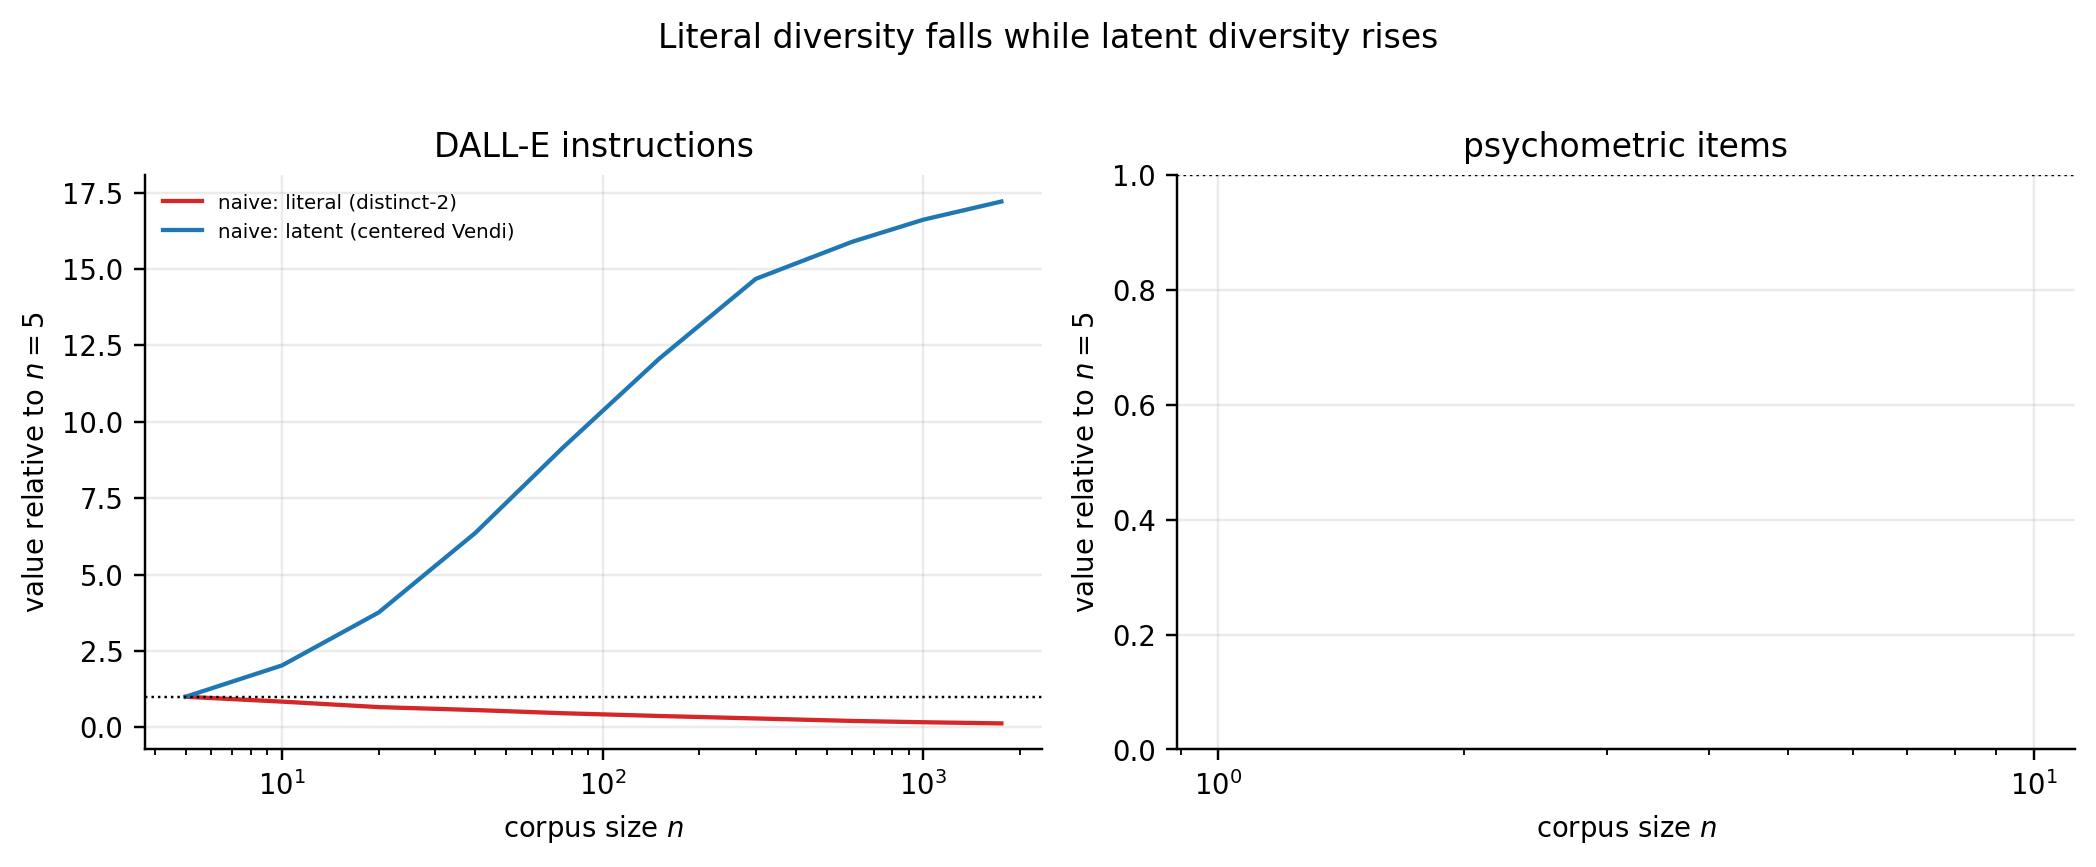
\includegraphics[keepaspectratio,alt={Figure 5. The decoupling, normalised to each series\textquotesingle{} value at n = 5: literal diversity falls while latent diversity rises.}]{figures/fig11_literal_vs_latent.png}}

\emph{Figure 5. The decoupling, normalised to each
series\textquotesingle{} value at n = 5: literal diversity falls while
latent diversity rises.}

\subsubsection{\texorpdfstring{7.6 Competitive comparison at matched
\emph{n}}{7.6 Competitive comparison at matched n}}\label{76-competitive-comparison-at-matched-n}

All seven arms, real corpora, DALL·E domain, every arm evaluated on the
same number of accepted items (\emph{n} = 200):

{\footnotesize
\begin{longtable}[]{@{}>{\raggedright\arraybackslash}p{\dimexpr 0.2827\linewidth-2\tabcolsep\relax}>{\raggedright\arraybackslash}p{\dimexpr 0.1283\linewidth-2\tabcolsep\relax}>{\raggedright\arraybackslash}p{\dimexpr 0.1414\linewidth-2\tabcolsep\relax}>{\raggedright\arraybackslash}p{\dimexpr 0.1571\linewidth-2\tabcolsep\relax}>{\raggedright\arraybackslash}p{\dimexpr 0.1371\linewidth-2\tabcolsep\relax}>{\raggedright\arraybackslash}p{\dimexpr 0.1533\linewidth-2\tabcolsep\relax}@{}}
\toprule\noalign{}
arm & distinct-2 ↑ & self-repetition ↓ & \emph{n}-gram Vendi ↑ &
centered Vendi ↑ & median NN distance ↑ \\
\midrule\noalign{}
\endhead
\bottomrule\noalign{}
\endlastfoot
naive & 0.293 & 0.345 & 107.6 & 50.45 & 0.045 \\
high temperature & 0.291 & 0.339 & 109.0 & 49.44 & 0.045 \\
Evol-Instruct & 0.386 & 0.353 & 108.1 & 50.10 & \textbf{0.021} \\
Self-Instruct & 0.545 & 0.131 & 140.4 & 67.45 & 0.121 \\
persona conditioning & 0.582 & 0.130 & 124.7 & 56.50 & 0.080 \\
\textbf{RAC} & 0.660 & 0.068 & 167.0 & 77.67 & 0.171 \\
\textbf{RAC + vision steering} & \textbf{0.699} & \textbf{0.040} &
\textbf{170.9} & \textbf{91.97} & \textbf{0.192} \\
\end{longtable}}

RAC wins every column, and adding vision steering improves on the
text-only variant by a further 18\% in centered Vendi. Three of the
baselines fail in different ways.

High temperature buys nothing here: distinct-2 of 0.291 against
naive\textquotesingle s 0.293, and an identical median nearest-neighbour
distance of 0.045. Turning the temperature up moved the third decimal
place, and moved it downward.

Evol-Instruct comes out worse than naive at the one thing a diversity
method exists for. Its median nearest-neighbour distance is 0.021,
against naive\textquotesingle s 0.045 --- it produces items
\emph{closer} to the existing corpus than independent sampling does. The
mechanism is working as designed: mutating an existing item produces a
neighbour of that item. Evol-Instruct raises \emph{distinct-2} (0.386 vs
0.293), because the mutations reword things, so a purely literal
evaluation would score it as an improvement. Measuring both levels is
what catches it.

Self-Instruct\textquotesingle s guard is literal, and it defends the
literal level only. It achieves the best self-repetition of any baseline
(0.131) (its ROUGE filter is doing real work), while its centered Vendi
(67.45) trails RAC by 10 points and RAC with vision steering by 24. A
ROUGE-L threshold cannot see semantic redundancy, and semantic
redundancy is what remains once the lexical kind is filtered.

\pandocbounded{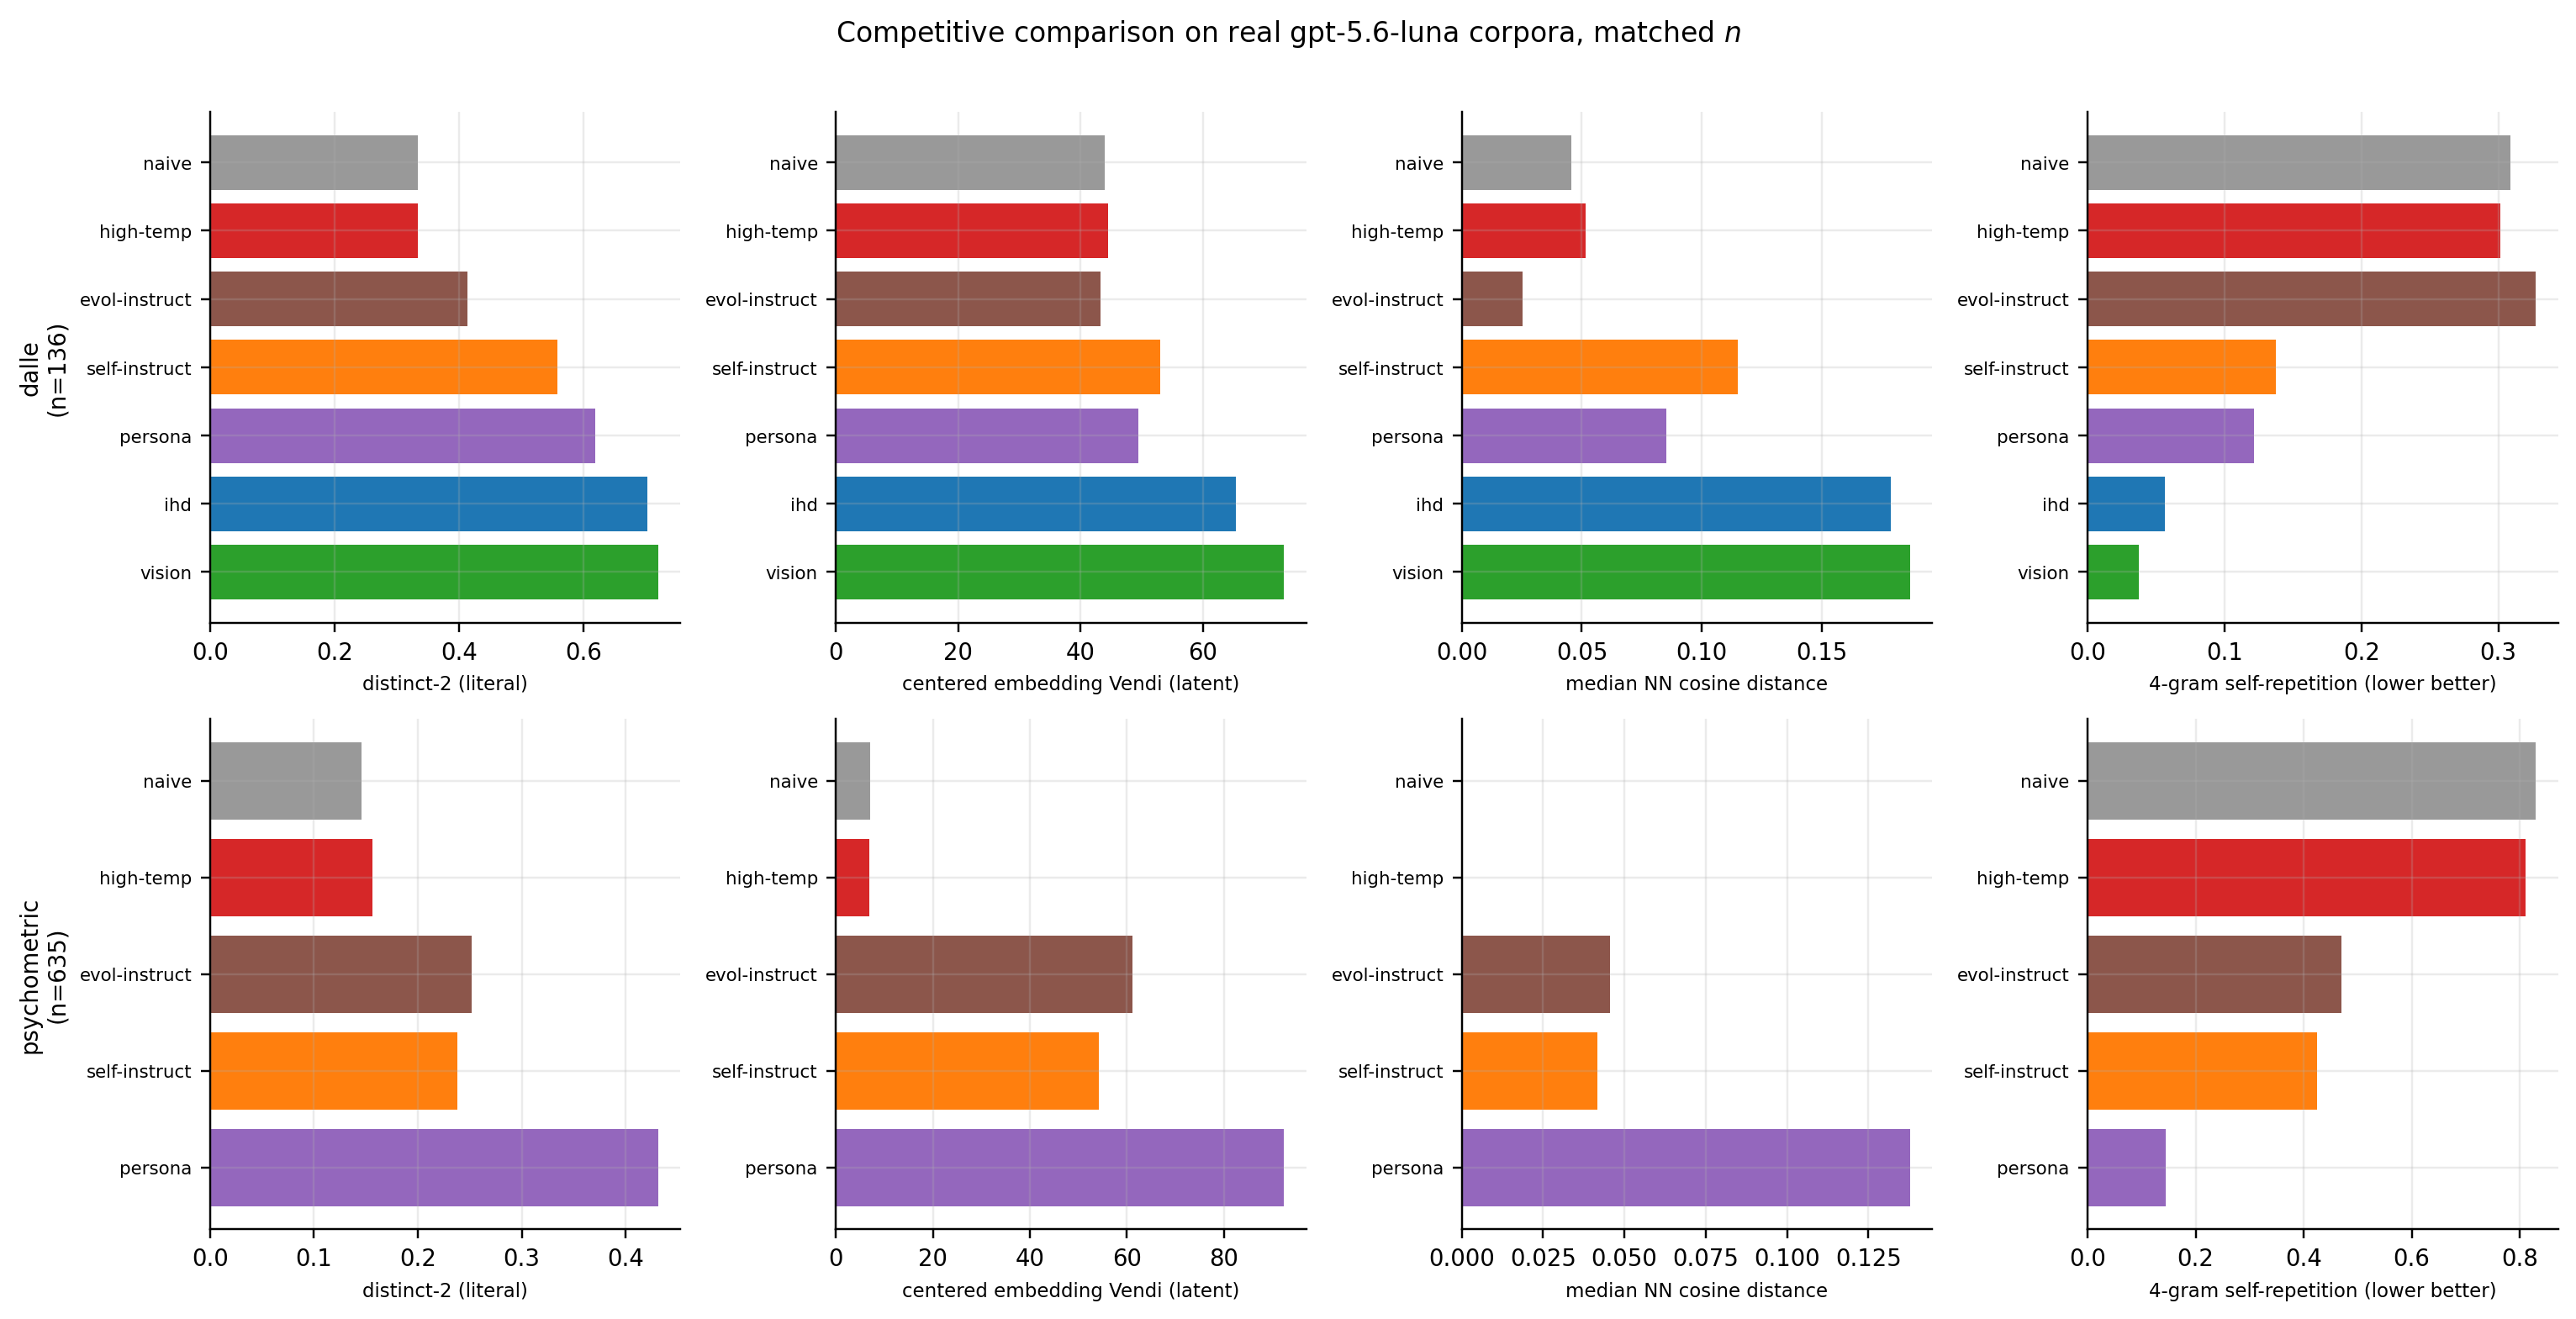
\includegraphics[keepaspectratio,alt={Figure 6. Competitive comparison on real corpora at matched n, both domains, across four metrics.}]{figures/fig14_arms.png}}

\emph{Figure 6. Competitive comparison on real corpora at matched n,
both domains, across four metrics.}

The psychometric domain repeats the ordering on all six arms at matched
\emph{n} = 1,058:

{\footnotesize
\begin{longtable}[]{@{}>{\raggedright\arraybackslash}p{\dimexpr 0.2506\linewidth-2\tabcolsep\relax}>{\raggedright\arraybackslash}p{\dimexpr 0.1137\linewidth-2\tabcolsep\relax}>{\raggedright\arraybackslash}p{\dimexpr 0.1137\linewidth-2\tabcolsep\relax}>{\raggedright\arraybackslash}p{\dimexpr 0.1253\linewidth-2\tabcolsep\relax}>{\raggedright\arraybackslash}p{\dimexpr 0.1393\linewidth-2\tabcolsep\relax}>{\raggedright\arraybackslash}p{\dimexpr 0.1216\linewidth-2\tabcolsep\relax}>{\raggedright\arraybackslash}p{\dimexpr 0.1359\linewidth-2\tabcolsep\relax}@{}}
\toprule\noalign{}
arm & exact-dup ↓ & distinct-2 ↑ & self-repetition ↓ & \emph{n}-gram
Vendi ↑ & centered Vendi ↑ & median NN distance ↑ \\
\midrule\noalign{}
\endhead
\bottomrule\noalign{}
\endlastfoot
naive & 0.668 & 0.114 & 0.855 & 11.8 & 7.1 & 0.000 \\
high temperature & 0.660 & 0.119 & 0.845 & 12.2 & 7.0 & 0.000 \\
Self-Instruct & 0.026 & 0.193 & 0.485 & 288.8 & 59.3 & 0.033 \\
Evol-Instruct & 0.025 & 0.224 & 0.470 & 307.4 & 75.0 & 0.047 \\
persona conditioning & 0.004 & 0.377 & 0.184 & 545.6 & 99.7 & 0.130 \\
\textbf{RAC} & \textbf{0.000} & \textbf{0.429} & \textbf{0.053} &
\textbf{644.3} & \textbf{124.8} & \textbf{0.210} \\
\end{longtable}}

RAC wins every column here as well. The two undiversified arms score an
order of magnitude worse on the latent measures because their duplicate
rates of 0.66--0.67 mean the embedding metric is largely measuring
repetition; deduplicating first raises them to 19.8 and 20.7, still far
behind every conditioned method, and their median nearest-neighbour
distance is exactly zero --- the median item has a perfect twin.

\subsubsection{7.7 Head-to-head against released instruction
corpora}\label{77-head-to-head-against-released-instruction-corpora}

We compare against the released corpora of the three most-used
synthetic-instruction methods --- Alpaca (Self-Instruct, 52k),
PersonaHub (50k), and WizardLM Evol-Instruct (143k) --- on scale-free
coverage of human-written instructions, together with a budget-matched
ablation of our own configurations.

\subsubsection{7.8 Protocol}\label{78-protocol}

Human-written reference: databricks-dolly-15k, split into two disjoint
3,000-item halves --- a STEER half that our method may read as
embeddings on the selection side, and an evaluation half that nothing in
any pipeline ever reads, and at which no corpus (ours or released) was
ever aimed. All scores below are on the evaluation half. Estimator:
Naeem et al. (2020) coverage/density with reference-side k-NN radii,
reported as AUC over k ∈ \{3, 5, 10, 20\}; radii are a property of the
reference alone, identical for every corpus, with nothing tunable per
corpus. Every corpus is evaluated as a uniform random sample at matched
\emph{n} = 450. Our arms and the reimplemented baselines all receive the
same 175 human seed tasks (the seed set Alpaca was built from), the same
generator, and the same budget of 2,400 generator calls --- rejection
and selection losses are counted, not hidden. The generator never sees a
reference word in any arm.

\subsubsection{7.9 The configuration}\label{79-the-configuration}

\begin{enumerate}
\def\labelenumi{\arabic{enumi}.}
\tightlist
\item
  \textbf{Aim by retrieval.} Sample an uncovered reference region
  (density-weighted, ∝ 1/r²), and retrieve the nearest texts we already
  own (seed tasks plus our own corpus) as the few-shot exemplars. The
  reference enters as embeddings on the steering side only; retrieval
  over owned text substitutes for the missing inverse oracle.
\item
  \textbf{Radius-adaptive mode.} The target\textquotesingle s own k-NN
  radius selects the prompt mode: tight radius (dense region)
  -\textgreater{} imitate the local task family closely; wide radius
  (sparse region) -\textgreater{} full diversification, with the nearest
  own outputs shown as explicit in-prompt negatives.
\item
  \textbf{Literal-channel spread.} Level-usage balancing across the
  elicited axis lattice (the headroom term applied at conditioning
  time), and a terse-register mandate.
\item
  \textbf{Keep everything.} Coverage is monotone in items; at a
  generation-matched budget, every discard is a permanent loss.
\end{enumerate}

\subsubsection{7.10 Results}\label{710-results}

\pandocbounded{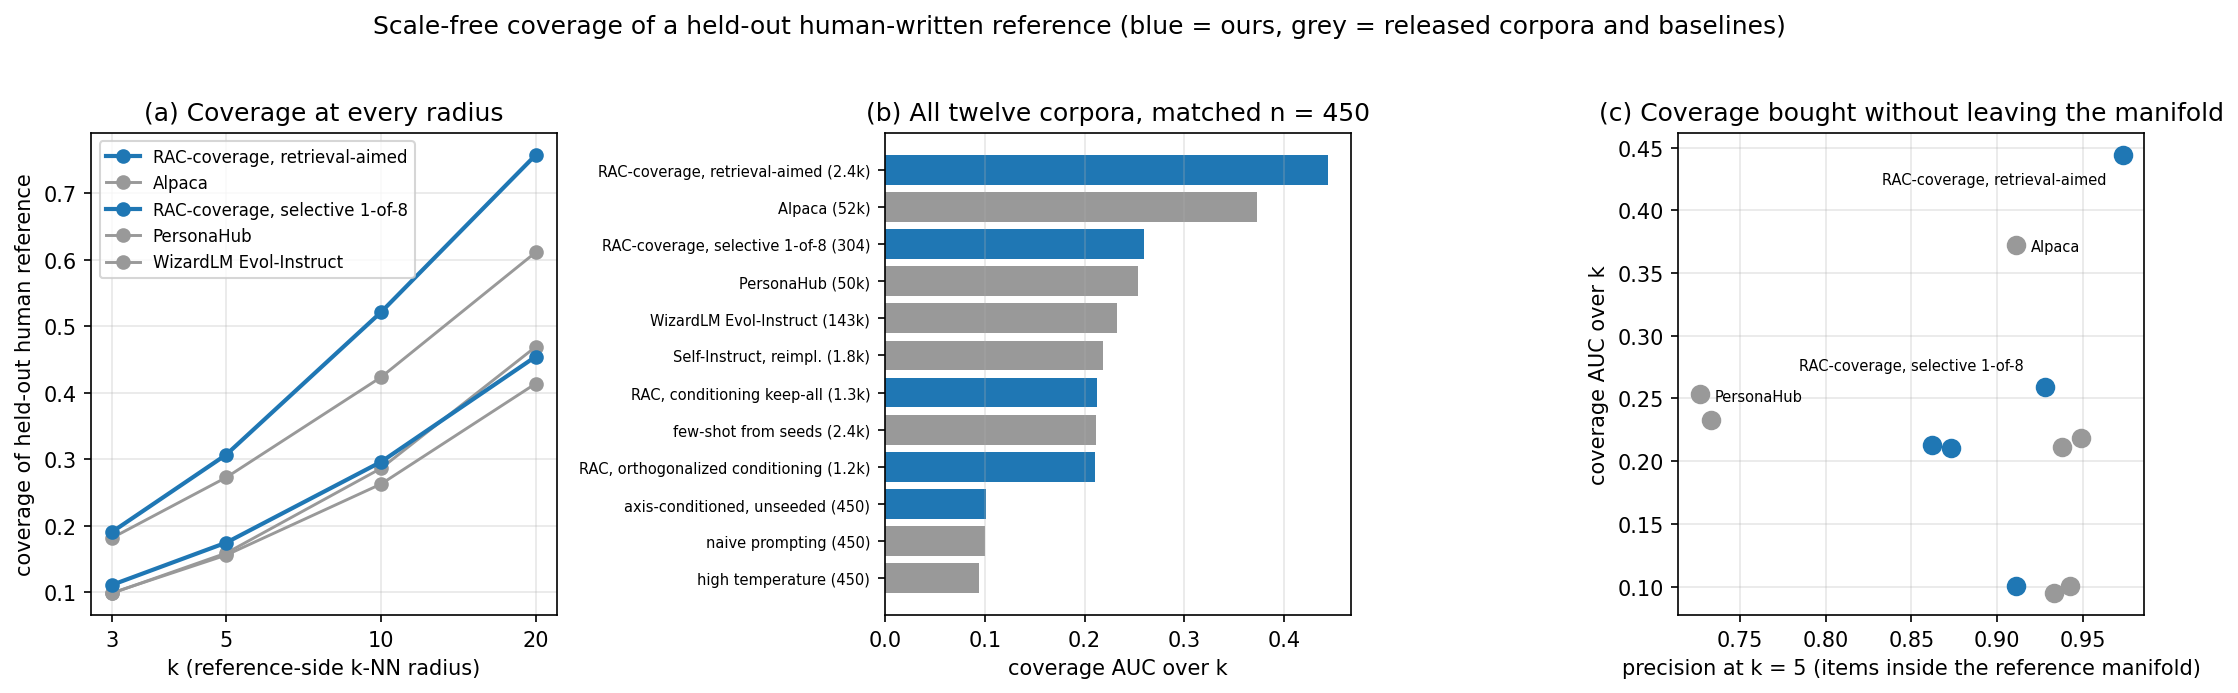
\includegraphics[keepaspectratio,alt={Figure 7. Scale-free coverage of a held-out human-written reference. (a) Coverage at every reference-side radius. (b) All twelve corpora at matched evaluated n = 450. (c) Coverage against precision: the winning corpus is also the one that stays inside the reference manifold.}]{figures/fig_h2h_scalefree.png}}

\emph{Figure 7. Scale-free coverage of a held-out human-written
reference. (a) Coverage at every reference-side radius. (b) All twelve
corpora at matched evaluated n = 450. (c) Coverage against precision:
the winning corpus is also the one that stays inside the reference
manifold.}

All twelve corpora, evaluation half, matched \emph{n} = 450:

{\footnotesize
\begin{longtable}[]{@{}>{\raggedright\arraybackslash}p{\dimexpr 0.3584\linewidth-2\tabcolsep\relax}>{\raggedright\arraybackslash}p{\dimexpr 0.3005\linewidth-2\tabcolsep\relax}>{\raggedright\arraybackslash}p{\dimexpr 0.1735\linewidth-2\tabcolsep\relax}>{\raggedright\arraybackslash}p{\dimexpr 0.1676\linewidth-2\tabcolsep\relax}@{}}
\toprule\noalign{}
rank & corpus & AUC & precision \\
\midrule\noalign{}
\endhead
\bottomrule\noalign{}
\endlastfoot
1 & \textbf{RAC-coverage, retrieval-aimed (2.4k)} & \textbf{0.4441} &
\textbf{0.973} \\
2 & Alpaca (Self-Instruct, 52k) & 0.3722 & 0.87 \\
3 & RAC-coverage, selective 1-of-8 (304) & 0.2591 & 0.93 \\
4 & PersonaHub (50k) & 0.2532 & 0.78 \\
5 & WizardLM Evol-Instruct (143k) & 0.2329 & 0.77 \\
6 & Self-Instruct (reimpl., same seeds/budget) & 0.2188 & \\
7 & RAC, conditioning keep-all & 0.2127 & \\
8 & few-shot from seeds & 0.2114 & \\
9 & RAC, orthogonalized conditioning & 0.2102 & \\
10 & axis-conditioned, unseeded & 0.1008 & \\
11 & naive & 0.1003 & \\
12 & high temperature & 0.0947 & \\
\end{longtable}}

Our method places first, 19\% above Alpaca, with the highest precision
in the field, at roughly one-twentieth of Alpaca\textquotesingle s
generation budget. An interim measurement at 22\% of budget (n = 528)
already scored 0.4276 against Alpaca\textquotesingle s 0.3666 on the
same protocol, so the result does not depend on final corpus size.
PersonaHub and WizardLM score below our selective arm despite 20--60×
the scale.

Budget-matched ablation (full corpora, 2,400 generator calls each, same
evaluation half):

{\footnotesize
\begin{longtable}[]{@{}>{\raggedright\arraybackslash}p{\dimexpr 0.3823\linewidth-2\tabcolsep\relax}>{\raggedright\arraybackslash}p{\dimexpr 0.0851\linewidth-2\tabcolsep\relax}>{\raggedright\arraybackslash}p{\dimexpr 0.1473\linewidth-2\tabcolsep\relax}>{\raggedright\arraybackslash}p{\dimexpr 0.1006\linewidth-2\tabcolsep\relax}>{\raggedright\arraybackslash}p{\dimexpr 0.1423\linewidth-2\tabcolsep\relax}>{\raggedright\arraybackslash}p{\dimexpr 0.1423\linewidth-2\tabcolsep\relax}@{}}
\toprule\noalign{}
configuration & kept & AUC & density & precision & recall \\
\midrule\noalign{}
\endhead
\bottomrule\noalign{}
\endlastfoot
\textbf{RAC-coverage, retrieval-aimed} & 2,398 & \textbf{0.6597} & 1.637
& \textbf{0.960} & \textbf{0.178} \\
Self-Instruct (reimpl.) & 1,833 & 0.3262 & 1.050 & 0.949 & 0.161 \\
few-shot from seeds & 2,399 & 0.3246 & 1.052 & 0.935 & 0.152 \\
conditioning, keep-all & 1,310 & 0.3147 & 0.704 & 0.864 & 0.068 \\
orthogonalized conditioning & 1,152 & 0.2941 & 0.718 & 0.873 & 0.101 \\
selective (1-of-8) & 304 & 0.2591 & 1.009 & 0.928 & 0.099 \\
\end{longtable}}

The ablation attributes the margin: retrieval-aiming and the
radius-adaptive mode carry it (rows 1 vs 2--4), few-shot anchoring to
the human seeds accounts for most of the baselines\textquotesingle{}
scores (row 3 vs the unseeded arms at 0.09--0.10),
Self-Instruct\textquotesingle s ROUGE filter adds 0.0016 over bare
few-shot, and both selection (row 6), and orthogonalized conditioning
(row 5) reduce coverage relative to keeping everything --- consistent
with §4: coverage is monotone and measure-seeking, so discarding and
occupied-span avoidance are each counter-productive under this
objective, whereas both are load-bearing under max-min.

\pandocbounded{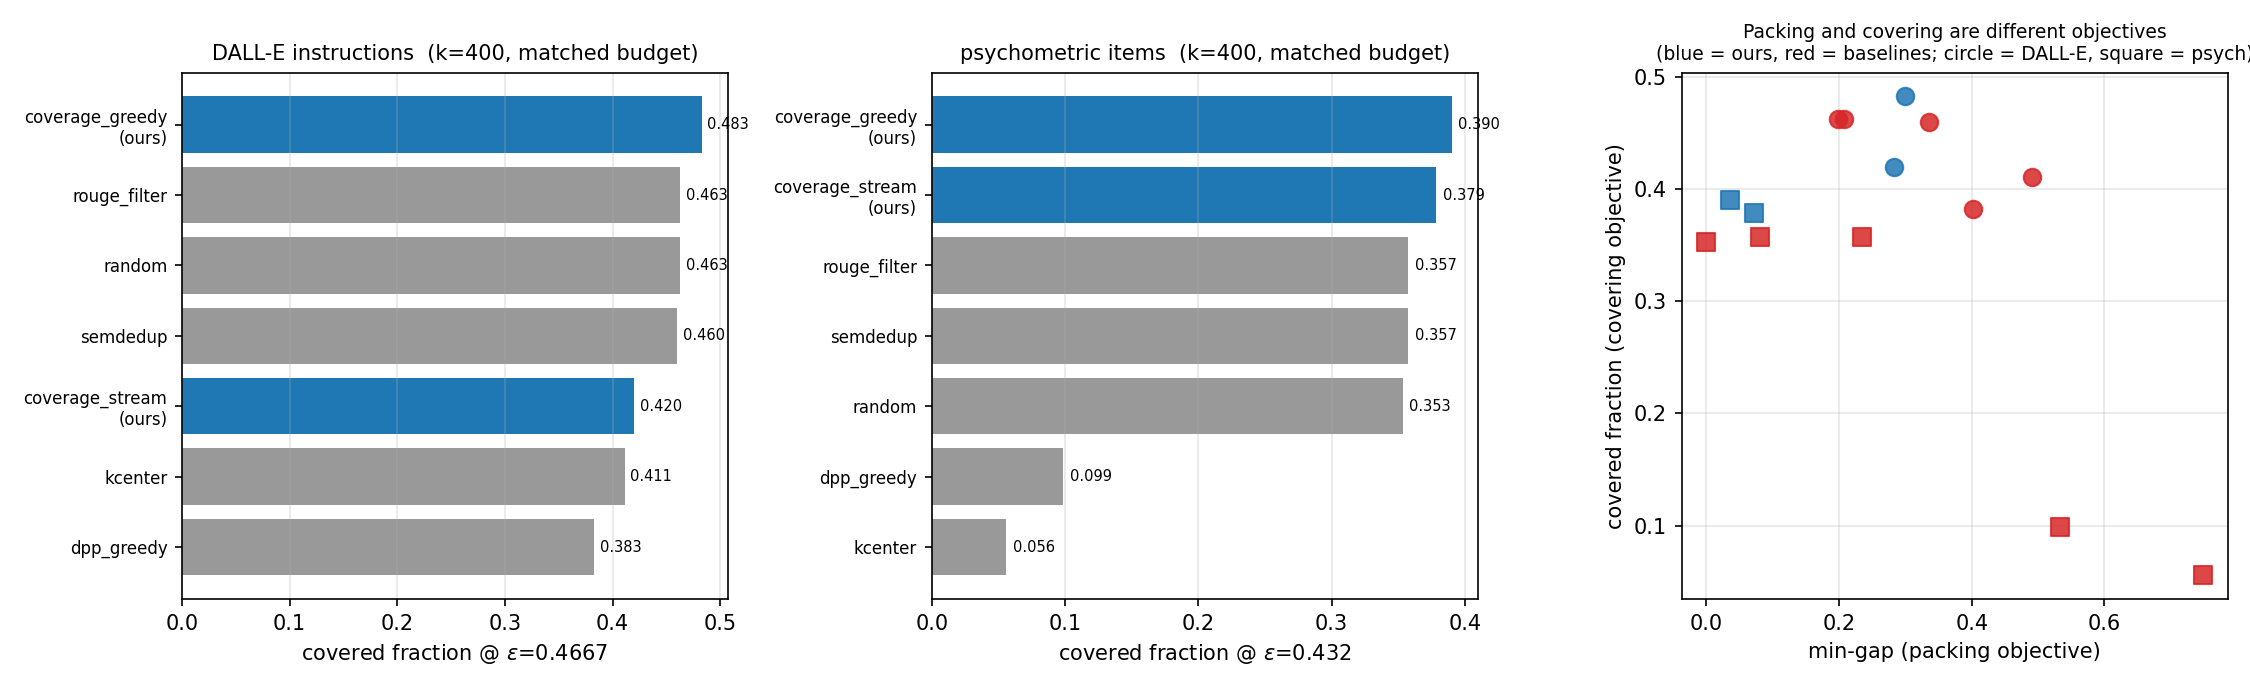
\includegraphics[keepaspectratio,alt={Figure 8. Selection benchmark: coverage-greedy against five literature baselines.}]{figures/fig_benchmark.png}}

\emph{Figure 8. Selection benchmark: coverage-greedy against five
literature baselines.}

\subsubsection{7.11 Notes}\label{711-notes}

A coverage number earns its place only if something a practitioner wants
depends on it. Three measurements say what does, on nine instruction
corpora scored against held-out human instructions no corpus was aimed
at.

\textbf{1. Four hundred items match a fifty-two-thousand-item corpus.}
Extending the retrieval-aimed policy to 24,000 generator calls and
measuring coverage as the corpus grows:

{\footnotesize
\begin{longtable}[]{@{}>{\raggedright\arraybackslash}p{\dimexpr 0.4174\linewidth-2\tabcolsep\relax}>{\raggedright\arraybackslash}p{\dimexpr 0.1990\linewidth-2\tabcolsep\relax}>{\raggedright\arraybackslash}p{\dimexpr 0.0514\linewidth-2\tabcolsep\relax}>{\raggedright\arraybackslash}p{\dimexpr 0.1542\linewidth-2\tabcolsep\relax}>{\raggedright\arraybackslash}p{\dimexpr 0.1780\linewidth-2\tabcolsep\relax}@{}}
\toprule\noalign{}
RAC items & coverage AUC & & RAC items & coverage AUC \\
\midrule\noalign{}
\endhead
\bottomrule\noalign{}
\endlastfoot
100 & 0.1878 & & 1,000 & 0.5394 \\
250 & 0.3023 & & 2,000 & 0.6323 \\
\textbf{400} & \textbf{0.3938} & & 5,000 & 0.7552 \\
500 & 0.4286 & & 10,000 & 0.8107 \\
750 & 0.5014 & & 13,978 & 0.8256 \\
\end{longtable}}

Alpaca\textquotesingle s full 52,002 items score 0.3722. \textbf{Four
hundred items of this corpus cover more of the reference than all of
Alpaca}, a ratio of 130 to 1, and at 13,978 items the corpus reaches
0.8256 --- 2.2× Alpaca\textquotesingle s coverage from 27\% of the
items. The per-thousand-item gain decays smoothly from 0.539 to 0.059,
which is the reachable support asserting itself exactly as §5 predicts:
the policy keeps finding new territory and keeps paying more for each
parcel.

\textbf{2. Seven times as many queries have a usable neighbour.} Take
each held-out instruction\textquotesingle s nearest neighbour in a
950-item pool from each corpus:

{\footnotesize
\begin{longtable}[]{@{}>{\raggedright\arraybackslash}p{\dimexpr 0.5294\linewidth-2\tabcolsep\relax}>{\raggedright\arraybackslash}p{\dimexpr 0.2235\linewidth-2\tabcolsep\relax}>{\raggedright\arraybackslash}p{\dimexpr 0.2471\linewidth-2\tabcolsep\relax}@{}}
\toprule\noalign{}
pool & mean NN similarity & queries served at 0.70 \\
\midrule\noalign{}
\endhead
\bottomrule\noalign{}
\endlastfoot
\textbf{RAC-coverage, retrieval-aimed} & \textbf{0.6224} &
\textbf{0.176} \\
Alpaca & 0.6164 & 0.118 \\
Persona-Hub (faithful) & 0.5921 & 0.038 \\
WizardLM Evol-Instruct & 0.5804 & 0.036 \\
RAC, orthogonalized conditioning & 0.5650 & 0.034 \\
RAC, conditioning keep-all & 0.5646 & 0.024 \\
\end{longtable}}

Pools of identical size, and the retrieval-aimed corpus serves 7.3× as
many queries as plain conditioning and 4.6× as many as the best
published baseline. Coverage AUC predicts this at \emph{r} = 0.972, and
mean neighbour similarity at \emph{r} = 0.983.

\textbf{3. The advantage grows with every demonstration retrieved.}
Retrieval matters only if better neighbours produce better answers.
Prompting a Qwen2.5-0.5B base model with \emph{k} retrieved
demonstrations per query --- no training anywhere, so the pool is the
only thing that differs --- and sweeping \emph{k}:

{\footnotesize
\begin{longtable}[]{@{}>{\raggedright\arraybackslash}p{\dimexpr 0.3127\linewidth-2\tabcolsep\relax}>{\raggedright\arraybackslash}p{\dimexpr 0.1514\linewidth-2\tabcolsep\relax}>{\raggedright\arraybackslash}p{\dimexpr 0.0957\linewidth-2\tabcolsep\relax}>{\raggedright\arraybackslash}p{\dimexpr 0.1354\linewidth-2\tabcolsep\relax}>{\raggedright\arraybackslash}p{\dimexpr 0.1173\linewidth-2\tabcolsep\relax}>{\raggedright\arraybackslash}p{\dimexpr 0.1875\linewidth-2\tabcolsep\relax}@{}}
\toprule\noalign{}
\emph{k} & RAC-coverage & Alpaca & RAC keep-all & RAC orth. & advantage
over keep-all \\
\midrule\noalign{}
\endhead
\bottomrule\noalign{}
\endlastfoot
1 & 0.1345 & 0.1422 & 0.1297 & 0.1178 & 1.04× \\
2 & 0.1363 & 0.1416 & 0.1162 & 0.1115 & 1.17× \\
4 & 0.1338 & 0.1468 & 0.0904 & 0.0782 & 1.48× \\
8 & \textbf{0.1186} & 0.1085 & 0.0499 & 0.0493 & \textbf{2.38×} \\
\end{longtable}}

At one demonstration the corpora are nearly indistinguishable. Every
additional slot widens the gap, and by eight the retrieval-aimed corpus
leads the field outright, Alpaca included, while the low-coverage pools
have collapsed to a third of their one-shot score. This is a
dose-response curve, and it is the strongest evidence here that coverage
is doing the work rather than accompanying it: a clustered pool exhausts
its distinct relevant demonstrations and begins repeating itself, and a
covering pool does not. Across corpora at \emph{k} = 4, coverage AUC
predicts in-context score at \emph{r} = 0.816.

\textbf{What this is for.} Demonstration pools for few-shot prompting,
retrieval corpora, evaluation suites, item banks --- any artifact
consulted by proximity to a query. On those, a corpus built this way is
worth roughly two orders of magnitude its size.

\textbf{What it is not for, and the limit of the evidence.} Fine-tuning
does not follow: coverage AUC against downstream fine-tuned quality is
\emph{r} = −0.166, and splitting by distance to the training set shows
why --- the retrieval-aimed corpus yields the best model on the third of
queries nearest its items (0.1960) and the worst on the third furthest
(0.1304), and a gradient step averages the two away.

Nor is coverage proven to be the \emph{cause} of the rankings above.
Three 800-item subsets drawn from a single corpus, differing only in
spread --- greedy-maximum (0.674 of the reference covered), random
(0.504), greedy-minimum (0.000) --- score 0.1409, 0.1456 and 0.1274: the
random subset edges the maximised one, and a nested ladder from the same
corpus is likewise non-monotone. What survives that test is that zero
coverage is clearly worst. Between corpora, coverage ranks them and the
dose-response follows the ranking; within one corpus, coverage alone
does not reproduce it, and the plausible reading is that greedy-maximum
selection favours outlying items, which fill holes in the space while
making poor demonstrations.

\subsubsection{7.12 A live coverage
pilot}\label{712-a-live-coverage-pilot}

\pandocbounded{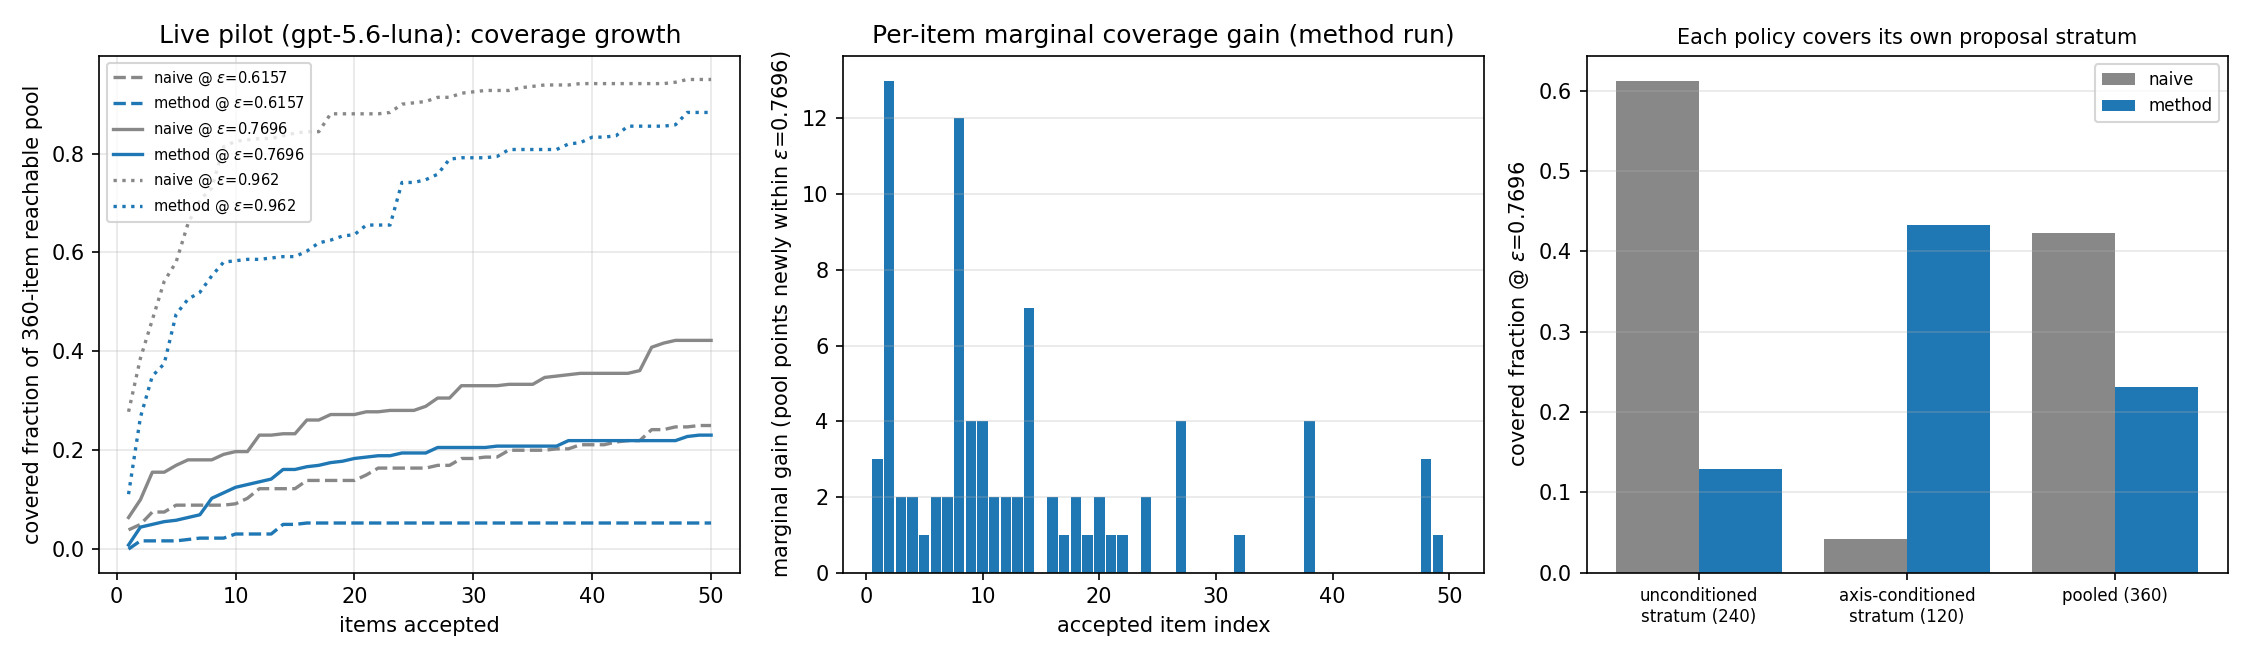
\includegraphics[keepaspectratio,alt={Figure 9. Live pilot: coverage and quality against budget.}]{figures/fig_live_pilot.png}}

\emph{Figure 9. Live pilot: coverage and quality against budget.}

\subsubsection{7.13 Setup and what it
cost}\label{713-setup-and-what-it-cost}

The pilot builds a red-team \emph{evaluation} prompt suite on the real
stack: gpt-5.6-luna via OpenRouter for generation, judging, attractor
mining and axis elicitation; local \texttt{nomic-embed-text} (768-d,
unit-normalized) for embeddings. Severity is deliberately mild --- the
items are benign user messages that probe whether an assistant adds
disclaimers, resists sycophancy and leading questions, and stays
calibrated, and the judge scores a \texttt{benign} dimension that
hard-gates acceptance. All state is append-only and checkpointed, so a
run is resumable after an interruption.

The run reached its full target: \textbf{50/50 accepted items} in 50
steps (K = 3 candidates each), against a \textbf{50-item naive baseline}
and a \textbf{360-item reference pool}. The pool has two strata --- 240
unconditioned one-shot draws and 120 axis-conditioned but
\emph{unselected} draws, because a reference pool must be drawn from the
same proposal process the policy uses, including every conditioning
mechanism. A pool of unconditioned draws alone sits outside the region
axis conditioning reaches (median distance 0.88, against a selection
radius of 0.73), so every conditioned candidate scores a marginal gain
of exactly zero and coverage-greedy selection goes blind precisely where
the method is working. Six axes were elicited, two refinements fired (8
axes final), and two ledger rounds mined attractors that became negative
constraints. Judge quality averaged 8.89/10. Cost of the final
instrumented segment: \textbf{74 calls, 36,056 prompt + 74,681
completion tokens, \$0.0968}, 394 s wall clock. Earlier segments (pool
construction, the naive baseline, and the first 32 accepts) predate the
usage ledger and are not included in that figure; total pilot spend was
well under the \$3 budget but only the final segment is \emph{measured},
so we report that number rather than an estimate.

\subsubsection{7.14 Literal versus latent diversity, and a kernel
caveat}\label{714-literal-versus-latent-diversity-and-a-kernel-caveat}

Tracking both n-gram and embedding diversity as the corpus grows
reproduces a divergence reported at much larger scale on this model
family: the two move in \textbf{opposite directions}.

{\footnotesize
\begin{longtable}[]{@{}>{\raggedright\arraybackslash}p{\dimexpr 0.3545\linewidth-2\tabcolsep\relax}>{\raggedright\arraybackslash}p{\dimexpr 0.1401\linewidth-2\tabcolsep\relax}>{\raggedright\arraybackslash}p{\dimexpr 0.1401\linewidth-2\tabcolsep\relax}>{\raggedright\arraybackslash}p{\dimexpr 0.1772\linewidth-2\tabcolsep\relax}>{\raggedright\arraybackslash}p{\dimexpr 0.1880\linewidth-2\tabcolsep\relax}@{}}
\toprule\noalign{}
n & distinct-1 & distinct-2 & Vendi (centered) & Vendi (uncentered) \\
\midrule\noalign{}
\endhead
\bottomrule\noalign{}
\endlastfoot
5 & 0.614 & 0.944 & 3.98 & 3.62 \\
10 & 0.482 & 0.861 & 8.01 & 5.04 \\
20 & 0.367 & 0.809 & 16.16 & 7.37 \\
30 & 0.338 & 0.791 & 23.65 & 10.00 \\
40 & 0.312 & 0.772 & 30.55 & 11.87 \\
50 & 0.295 & 0.770 & 37.06 & 13.54 \\
\end{longtable}}

Literal diversity falls monotonically (distinct-2 0.944 → 0.770), while
latent diversity rises monotonically (centered Vendi 3.98 → 37.06).
Reporting either alone supports an opposite conclusion about the same
corpus. The mechanism is plain enough --- a growing corpus reuses
vocabulary and sentence frames while still spreading in meaning-space,
but it means "diversity" must be qualified by level, and a coverage
objective defined on embeddings is silent about literal repetition.
(Against the naive baseline the method is slightly \emph{less} literally
diverse at distinct-1, 0.295 vs 0.341, and slightly more diverse
latently, centered Vendi 37.06 vs 30.34, with markedly lower
self-repetition, max 3-gram Jaccard 0.036 vs 0.083.)

The uncentered Vendi is a kernel artifact. Same-domain embeddings share
a mean direction, and an uncentered linear kernel measures that shared
cone as if it were content. On this data the two readings differ by 2.7×
(13.54 vs 37.06) and, worse, they order the growth curve differently in
slope. We report both everywhere and treat only \emph{relative}
comparisons at fixed n as defined for the uncentered form.

Is ε measuring the cone or the content?. This is the question the caveat
raises for every coverage number computed with cosine distances, so we
measured it. Our pool\textquotesingle s mean pairwise cosine is
\textbf{0.444} (p05 0.330, p95 0.591) (a wide cone, not the
\textasciitilde0.9 concentration seen in some same-domain embedding
sets) with mean direction norm 0.667. Our ε\_sel = 0.770 corresponds to
cosine similarity 0.704, which sits at the \textbf{1.8th percentile} of
pairwise distances: an ε-ball at this radius captures genuine
near-duplicates, not the bulk of the cone. So for this pilot the
coverage numbers are measuring content. We record the diagnostic because
the answer is embedder- and domain-dependent: with a tighter cone the
same calibration rule would have produced an ε inside the
cone\textquotesingle s width, and the resulting "coverage" would have
been a restatement of the embedding geometry. Any coverage result
computed on cosine distances should publish this check.

\subsubsection{7.15 The proxy problem: text diversity is nearly blind to
image
diversity}\label{715-the-proxy-problem-text-diversity-is-nearly-blind-to-image-diversity}

We rendered the first 199 DALL·E instructions from the naive corpus to
actual images and embedded them with CLIP. The result is the most
consequential measurement in this section:

\begin{quote}
Pairwise cosine similarity in text-embedding space correlates with
pairwise cosine similarity in image-embedding space at \textbf{Pearson
\emph{r} = 0.170}.
\end{quote}

Knowing that two instructions are semantically far apart tells you very
nearly nothing about whether the two pictures look different. Every
text-side diversity method in the table above (ours included) is
optimizing a proxy that explains roughly 2\% of the variance in the
thing the user actually receives.

The qualitative version is more damning than the correlation.
Independently generated instructions, from a corpus with a 0.000
exact-duplicate rate and healthy lexical diversity, render to
near-interchangeable pictures (Figure 11, top): the same
magenta-and-cyan palette, a classical marble bust, neon signage,
halftone collage, a receding grid. A vision judge shown samples of the
set rates its distinctness 6--7 out of 10 and names the attractors
precisely --- \emph{"muted beige, cream, brown, ochre and black
foundations accented by saturated cyan/teal, turquoise, pink"},
\emph{"appropriation of canonical or religious imagery, especially Mona
Lisa-like female portraits"}, \emph{"frontal, museum-like presentation
with centered, symmetrical compositions"}.

This is a second mode collapse, downstream of ours, contributed by the
image model and by the fact that much of what varies in the text
("post-modern", "appropriated source") lands in the same visual place.

\pandocbounded{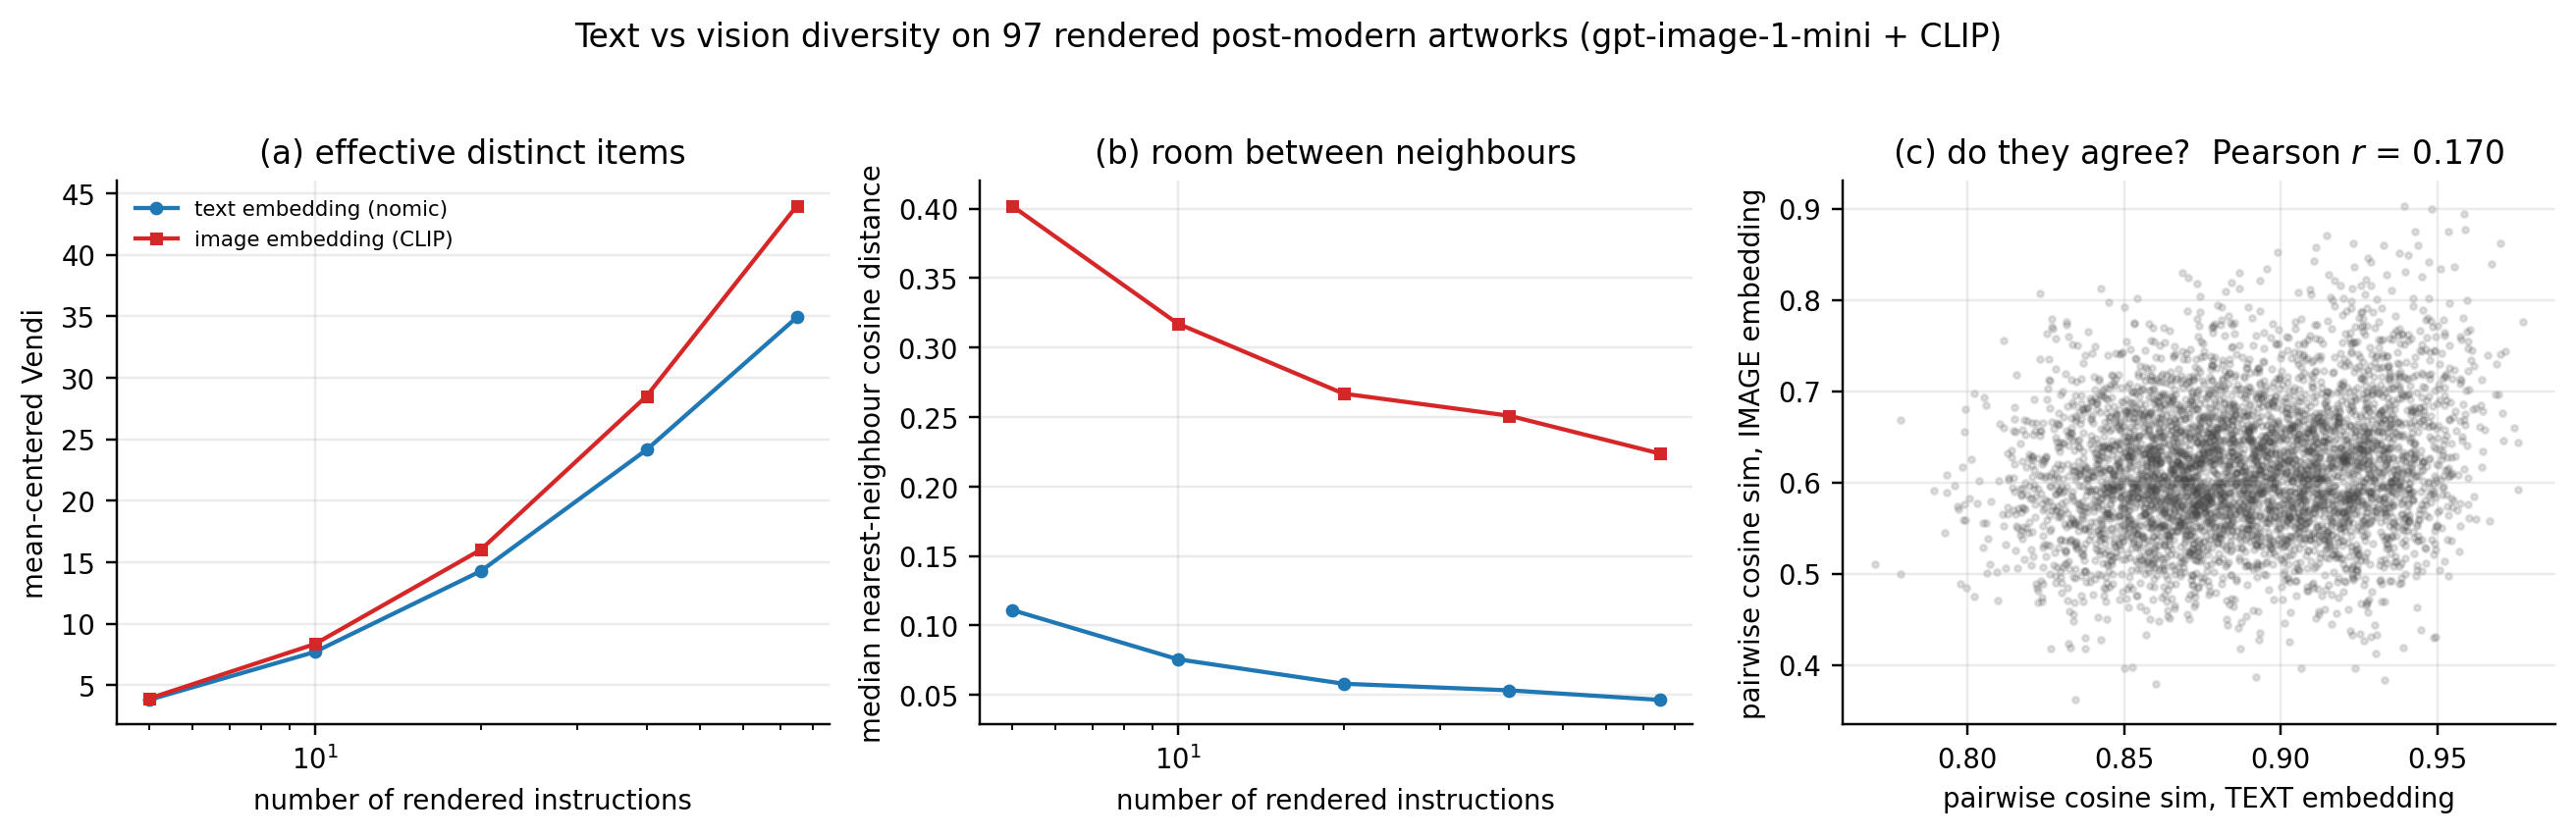
\includegraphics[keepaspectratio,alt={Figure 10. Text versus vision diversity on 97 rendered artworks. (c) Pairwise similarities in the two spaces correlate at only r = 0.170.}]{figures/fig12_vision.png}}

\emph{Figure 10. Text versus vision diversity on 97 rendered artworks.
(c) Pairwise similarities in the two spaces correlate at only r =
0.170.}

\pandocbounded{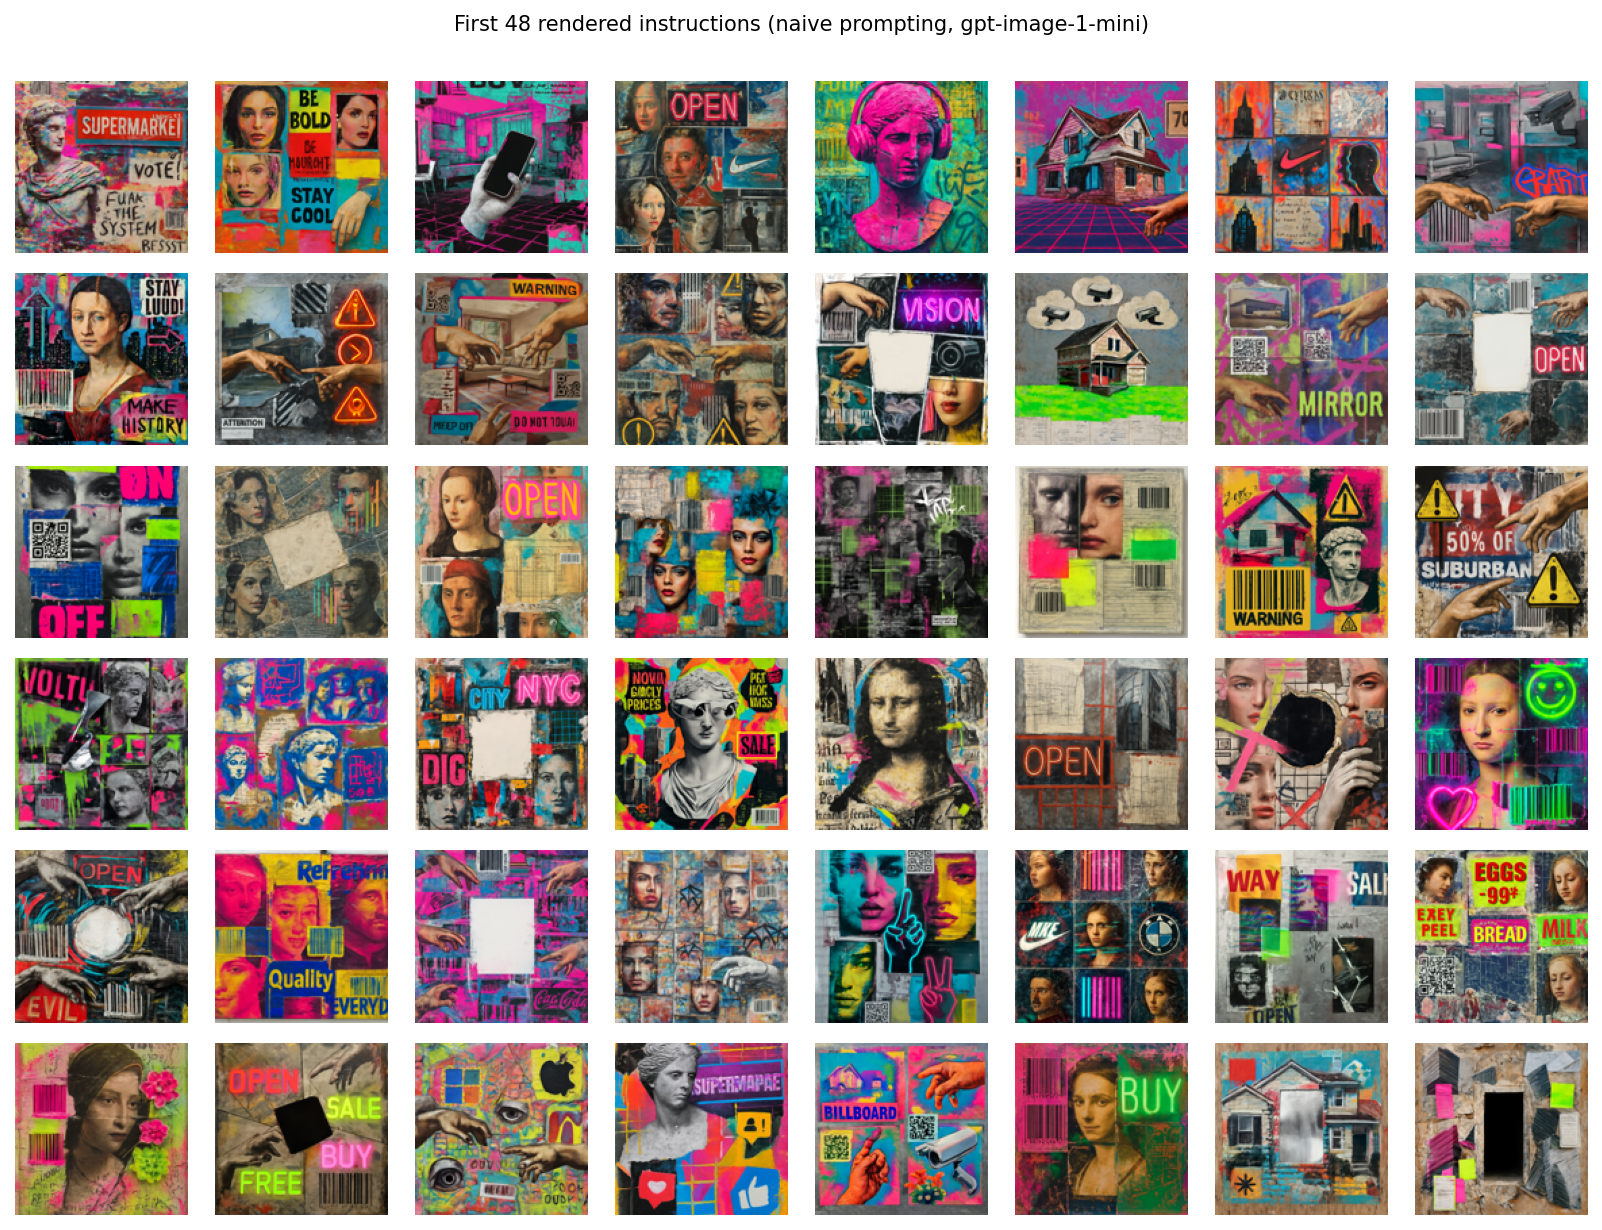
\includegraphics[keepaspectratio,alt={Figure 11. Sixteen renders per policy, same generator, same budget, same image model. Rows 1--2, naive prompting: a corpus with a 0.000 exact-duplicate rate and healthy lexical diversity that still returns one visual mode, with magenta and cyan collage, barcodes and QR codes, Renaissance portraits and classical busts, Michelangelo hands, warning triangles and neon OPEN signs recurring across nearly every panel. Rows 3--4, max-min steering with literal and latent repulsion on both the text and vision sides: medium, palette, register and composition all move, across a medieval triptych, a botanical cabinet, a photographed sculpture installation, a torn-paper abstract and a civic notice. Tiling survives the steering: 38\% of the steered renders still score as literal tilings and 42\% still share a palette with a nearest neighbour, which §7.15 and §7.20 quantify.}]{figures/fig13_contact_sheet.png}}

\emph{Figure 11. Sixteen renders per policy, same generator, same
budget, same image model. Rows 1--2, naive prompting: a corpus with a
0.000 exact-duplicate rate and healthy lexical diversity that still
returns one visual mode, with magenta and cyan collage, barcodes and QR
codes, Renaissance portraits and classical busts, Michelangelo hands,
warning triangles and neon OPEN signs recurring across nearly every
panel. Rows 3--4, max-min steering with literal and latent repulsion on
both the text and vision sides: medium, palette, register and
composition all move, across a medieval triptych, a botanical cabinet, a
photographed sculpture installation, a torn-paper abstract and a civic
notice. Tiling survives the steering: 38\% of the steered renders still
score as literal tilings and 42\% still share a palette with a nearest
neighbour, which §7.15 and §7.20 quantify.}

A reader looking at rows 3 and 4 of Figure 11 will notice that they
still favour grids, panels and tiled compositions more than a human art
director would, and the structural audit agrees: 38\% of those renders
score above 0.5 on the autocorrelation tiling measure. That is what the
objective asks for and no more. A max-min corpus is scored on how far
apart its items are, and nothing in the score says the corpus should
look like any particular distribution of artworks --- there is no
likelihood term, no reference set, no penalty for sitting in a region of
image space that real post-modern art rarely occupies. If the
generator\textquotesingle s prior happens to place a whole family of
mutually distant images inside the tiled-grid region, spreading points
is satisfied by staying there and varying what fills the cells. The
covering objective is the one that has a reference distribution in it,
and a corpus scored on coverage of human-written material inherits a
pull toward where that material actually sits. Buying both at once means
carrying both terms, which is a different optimization from the one
measured here.

The vision-steered arm closes the loop where the product actually lives.
It renders a bounded sample of accepted instructions, embeds them with
CLIP, and feeds two things back into the text-side loop: a least-squares
map from the crowded \emph{image} directions into instruction-embedding
space, so the text-side orthogonality term can push away from visual
redundancy it cannot itself perceive; and mined \emph{visual} attractors
from the vision judge, appended to the same append-only ledger as the
textual ones and repelled against in subsequent prompts. It is the
paper\textquotesingle s mechanism applied one level down: the ledger
already repels against what the model keeps saying, and now also against
what it keeps showing. It is the best arm in the table.

\subsubsection{7.16 Attractor mining works, and is
legible}\label{716-attractor-mining-works-and-is-legible}

The mining step produces findings specific enough to act on. From the
poetry pilot, round 1 (\emph{n} = 25): \emph{"self-correction and
immediate retraction: speakers repeatedly interrupt their own claims"};
\emph{"ceremonial or institutional address: the voice of a bell-ringer,
town crier, registrar, witness"}; \emph{"threshold imagery and delayed
passage: doors, gates, windows, bridges, shores"}. By round 2 (\emph{n}
= 50) it tracks the corpus\textquotesingle s \emph{drift} rather than
restating round 1, noting that technical vocabulary is now being placed
inside mythic frames and that recursive epistemic backtracking has
become structural.

These findings are nameable and therefore repellable, which is what
makes them usable as prompt constraints; a finding of "similar tone"
would not be. And several of them are artifacts of \emph{our own axis
elicitation} --- asking for craft-level axes like "relationship to its
own claim" reliably produces self-correcting speakers. \textbf{The
system\textquotesingle s own conditioning becomes the next attractor.}
The ledger catches the system\textquotesingle s own habits alongside the
model\textquotesingle s.

\subsubsection{7.17 The exam bank: a judged enemy-item
radius}\label{717-the-exam-bank-a-judged-enemy-item-radius}

Exam items invert the semantics of the other two domains. Two
operational items closer than δ are \emph{enemy items} (seeing one gives
away the other) a test-security failure at any bank size, so the floor
is a hard constraint rather than a term in a weighted sum, and the
min-distance check must be exact against the full bank rather than
subsampled. Item templates expose few manipulable slots, so each mode is
a low-dimensional disk and the δ-packing number of a bank is finite and
small: a bank has a capacity, and the operative question is what
fraction of a nominal bank is actually usable. That turns on δ, so we
measured it. 236 item pairs drawn from a human-written bank (MMLU)
across the full range of embedding distance were put to a blind
psychometric adjudication --- does seeing one item give a material
advantage on the other, through a shared fact, a re-skin, or matched
distractor misconceptions --- with the judge shown neither the distance
nor the provenance. A logistic fit of enemy verdicts on distance crosses
50\% at \textbf{δ = 0.0354}, which is the operative radius for this
embedder and item type.

Applying that radius to real banks --- six generation policies at 2,500
items each, and the human bank under identical treatment:

{\footnotesize
\begin{longtable}[]{@{}>{\raggedright\arraybackslash}p{\dimexpr 0.4121\linewidth-2\tabcolsep\relax}>{\raggedright\arraybackslash}p{\dimexpr 0.1692\linewidth-2\tabcolsep\relax}>{\raggedright\arraybackslash}p{\dimexpr 0.1971\linewidth-2\tabcolsep\relax}>{\raggedright\arraybackslash}p{\dimexpr 0.2216\linewidth-2\tabcolsep\relax}@{}}
\toprule\noalign{}
bank & exact-dup & items with an enemy & usable after the floor \\
\midrule\noalign{}
\endhead
\bottomrule\noalign{}
\endlastfoot
MMLU (human-written) & 0.024 & 0.092 & 2,373 (94.9\%) \\
naive prompting & 0.695 & 0.884 & 382 (15.3\%) \\
high temperature & 0.710 & 0.897 & 365 (14.6\%) \\
Self-Instruct & 0.047 & 0.616 & 1,373 (54.9\%) \\
Evol-Instruct & 0.012 & 0.424 & 1,870 (74.8\%) \\
persona conditioning & 0.007 & 0.047 & 2,425 (97.0\%) \\
\textbf{RAC} & \textbf{0.000} & \textbf{0.000} & \textbf{1,058
(100.0\%)} \\
\end{longtable}}

A naively generated bank of 2,500 items yields 382 that can coexist on
one form --- 15\% of nominal capacity, against 94.9\% for the human
bank. Temperature makes it slightly worse. Both conditioned policies
exceed the human bank\textquotesingle s usable fraction, and the
axis-conditioned bank contains no enemy pair at all at the judged
radius, though it is measured at 1,058 items rather than 2,500 and the
comparison should be read at that size.

\subsubsection{7.18 Head-to-head against a human-written exam
bank}\label{718-head-to-head-against-a-human-written-exam-bank}

The comparisons above are against our own reimplementations, which is
the right experiment for isolating mechanisms and the wrong one for the
question \emph{is this actually good?} --- a reimplementation can be
weak in ways that flatter us. So we also compare against an item bank
that humans wrote: \textbf{MMLU}, \textasciitilde14,000 multiple-choice
items drawn from real practice exams and textbooks across 57 subjects,
by many authors, with editorial review, over years. All arms are sampled
uniformly at random and evaluated at matched \emph{n} = 1,000 with
identical metric code.

{\footnotesize
\begin{longtable}[]{@{}>{\raggedright\arraybackslash}p{\dimexpr 0.2817\linewidth-2\tabcolsep\relax}>{\raggedright\arraybackslash}p{\dimexpr 0.1138\linewidth-2\tabcolsep\relax}>{\raggedright\arraybackslash}p{\dimexpr 0.1138\linewidth-2\tabcolsep\relax}>{\raggedright\arraybackslash}p{\dimexpr 0.1211\linewidth-2\tabcolsep\relax}>{\raggedright\arraybackslash}p{\dimexpr 0.1346\linewidth-2\tabcolsep\relax}>{\raggedright\arraybackslash}p{\dimexpr 0.1175\linewidth-2\tabcolsep\relax}>{\raggedright\arraybackslash}p{\dimexpr 0.1175\linewidth-2\tabcolsep\relax}@{}}
\toprule\noalign{}
source & exact-dup ↓ & distinct-2 ↑ & self-repetition ↓ & \emph{n}-gram
Vendi ↑ & centered Vendi ↑ & median NN dist ↑ \\
\midrule\noalign{}
\endhead
\bottomrule\noalign{}
\endlastfoot
\textbf{MMLU (human-written)} & 0.0040 & \textbf{0.5888} & 0.0585 &
495.2 & \textbf{197.50} & \textbf{0.2838} \\
naive gpt-5.6-luna & 0.6560 & 0.1196 & 0.8383 & 12.1 & 6.52 & 0.0000 \\
high temperature & 0.6840 & 0.1161 & 0.8567 & 10.2 & 6.66 & 0.0000 \\
Self-Instruct & 0.0280 & 0.1990 & 0.4797 & 277.6 & 57.22 & 0.0351 \\
Evol-Instruct & 0.0060 & 0.2642 & 0.3855 & 381.9 & 89.23 & 0.0792 \\
persona conditioning & 0.0040 & 0.3887 & 0.1711 & 543.3 & 99.71 &
0.1346 \\
\textbf{RAC} & \textbf{0.0000} & 0.4377 & \textbf{0.0503} &
\textbf{622.2} & 135.58 & 0.2235 \\
\end{longtable}}

The synthetic and human comparisons come out differently, and the
difference matters.

Against every synthetic method, RAC wins every column. Centered Vendi
135.6 against the best baseline\textquotesingle s 99.7 --- a 36\% margin
over persona conditioning, which is the closest published relative of
our approach and differs from it exactly by the three components we add.
Self-repetition 0.050 against persona\textquotesingle s 0.171. The
undiversified arms are not close: naive and high-temperature prompting
score \textasciitilde6.5 centered Vendi, because two-thirds of their
corpora are byte-identical duplicates, and their median
nearest-neighbour distance is exactly 0.0000 --- the median item has a
perfect twin.

Against the human bank the result splits. We \emph{beat} MMLU on exact
duplication (0.0000 vs 0.0040 --- the human bank has some), on 4-gram
self-repetition (0.050 vs 0.059), and on \emph{n}-gram Vendi (622 vs
495): our items reuse less language than human-written ones do. We
\emph{lose} on the semantic measures --- centered Vendi 135.6 against
197.5, and median nearest-neighbour distance 0.224 against 0.284. We
reach roughly 69\% of a human exam bank\textquotesingle s effective
semantic diversity.

That gap is the honest measure of what is left. MMLU\textquotesingle s
spread comes from 57 genuinely different subjects; ours comes from an
axis lattice a single model proposed in one call, refined a handful of
times. The lexical result says our surface variety already exceeds
human-authored items; the semantic result says our \emph{conceptual}
variety does not, and that closing the remaining 31\% is a question
about how much genuinely different subject matter the generator can be
induced to reach, which is precisely the reachable-dimension question of
§5, not a tuning problem.

\subsubsection{7.19 Which metrics are independent of the
objective}\label{719-which-metrics-are-independent-of-the-objective}

Our selection rule maximizes a weighted sum of embedding-space
orthogonality and embedding-space min-gap. We then report
embedding-space diversity metrics. Those two facts are not independent:
the centered Vendi Score is a monotone function of how flat the
embedding Gram spectrum is, which is close to exactly what the
orthogonality term climbs, and the median nearest-neighbour distance
\emph{is} the min-gap term. To that extent, the wins on centered Vendi
and median nearest-neighbour distance are partly tautological: the
method optimizes them and the baselines do not, so they should be read
as confirmation that the optimizer works rather than as independent
evidence.

The independent evidence is that the method never observes the
\emph{literal} metrics at all. It reads embeddings; it has no access to
token counts, \emph{n}-gram overlap, or string identity. So
exact-duplicate rate, distinct-2, 4-gram self-repetition, and
\emph{n}-gram Vendi are independent of the objective in a way the
embedding metrics are not, and the method wins those too, including
against the human-written bank on two of the four. Sorted by how much
weight they can bear:

\begin{itemize}
\tightlist
\item
  \textbf{Embedding-space measures (Vendi, NN distance):} partly
  circular; confirmation that the optimizer works.
\item
  \textbf{Literal-space measures (duplication, distinct-2,
  self-repetition, \emph{n}-gram Vendi):} independent, since nothing in
  the method targets them. These carry the argument.
\item
  \textbf{Rendered-artifact measures (CLIP, CLAP, MERT):} the most
  independent, living downstream of a second generative model the method
  never sees, which is why §7.15 matters more than its length suggests.
\end{itemize}

A reader who trusts only the third category still has the \emph{r} =
0.170 result, which is a finding about every method in the table rather
than a comparison between them.

\subsubsection{7.20 Literal-space repulsion: fixing what the embeddings
cannot
see}\label{720-literal-space-repulsion-fixing-what-the-embeddings-cannot-see}

Embedding metrics miss an entire class of repetition: tiled grids of one
cell, prominent typography, a single shared palette, the same
composition recolored. Audited with deliberately dumb, non-semantic
signatures (a 16×16 luminance layout map, an autocorrelation tiling
score, a hue histogram): half the images had a layout twin above 0.5
cosine, 40--45\% were literal tilings, and 63--78\% shared a palette,
while prompt-level Jaccard sat at a healthy 0.14--0.17. Varied words,
one visual mode: the conditional-dimension gap operating inside the
\emph{renderer}.

The fix is a four-quadrant repulsion (\{text, vision\} × \{literal,
latent\}) where the two literal quadrants were previously unpopulated:
content-word overlap penalties and live overused-word bans on the text
side; and on the vision side, measured structural bans injected into
prompts (grids banned when recent renders tile, dominant hue pairs named
and banned, layout-change demands when layouts collide), plus a learned
text→bad-structure bridge that penalizes candidates near prompts whose
renders tiled. Rerun at matched budget, palette twins halved (0.78 →
0.35 in the coverage arm), the coverage objective improved 21\% (0.206 →
0.247), and layout/tiling moved modestly (0.51 → 0.46--0.48; 0.45 →
0.33) --- a partial improvement, with the residue attributable to the
image model\textquotesingle s own prior resisting text-side instruction.

\subsubsection{7.21 Audio: prompts, the steered corpus, and embedder
dependence}\label{721-audio-prompts-the-steered-corpus-and-embedder-dependence}

\textbf{Prompt-level diversity.} At matched \emph{n}, matched prompt
length and the same generator, the conditioned arm reaches centered
Vendi 43.03 against naive\textquotesingle s 22.99 (1.87×), halves 4-gram
self-repetition (0.140 vs 0.291), raises distinct-2 (0.545 vs 0.348) and
\emph{n}-gram Vendi (75.3 vs 56.0), and holds roughly three times the
room between nearest neighbours (0.079 vs 0.027), on 100 prompts per
arm. Neither arm produces exact duplicates, so the effect is semantic.
This replicates on a third artifact type the pattern of §7.4 and §7.6:
conditioning moves the number, sampling temperature does not.

\textbf{The steered corpus.} 100 Lyria-3-Pro instrumentals generated by
cross-modal steering with zero rejection --- selection happens over
prompts, every render is kept. Final measurements: 100\% of tracks
verify as instrumental in CLAP space (minimum instrumental-vs-vocal
margin 0.077); mean-centered CLAP Vendi 17.43, against 11.5 (naive
prompts), and 14.1 (axis-conditioned prompts) for the unsteered 47-track
arms under the same embedder; opening loudness at 0.72 of each
track\textquotesingle s own median over the first three seconds, against
a 0.46--0.61 baseline --- the sparse-opening attractor substantially,
not fully, suppressed.

\textbf{Structural control.} Lyria honors its own section-marker format
(\texttt{{[}{[}A0{]}{]}\ {[}{[}B1{]}{]}\ …}), and ignores wall-clock
timestamps. Compliance with a requested section sequence is
length-dependent: exact at prompt lengths near 560 characters, 0.11 at a
mean of 658, zero by \textasciitilde1,600. Structural contracts for
music must be short or they are noise.

Whether a prompt can be steered before rendering turns out to be a
property of the embedder rather than of music. Prompt-to-track alignment
(Spearman between prompt-pair similarity through the text tower and
track-pair similarity through the audio tower, naive/conditioned arms):

{\footnotesize
\begin{longtable}[]{@{}>{\raggedright\arraybackslash}p{\dimexpr 0.4402\linewidth-2\tabcolsep\relax}>{\raggedright\arraybackslash}p{\dimexpr 0.1969\linewidth-2\tabcolsep\relax}>{\raggedright\arraybackslash}p{\dimexpr 0.3630\linewidth-2\tabcolsep\relax}@{}}
\toprule\noalign{}
embedder & alignment & note \\
\midrule\noalign{}
\endhead
\bottomrule\noalign{}
\endlastfoot
\textbf{MuQ-MuLan} (open MuLan-style) & \textbf{0.68 / 0.47} & a usable
steering gradient \\
CLAP-fused & 0.50 / 0.21 & weak; \textasciitilde0.05 on the steered
corpus \\
CLAP-music & 0.18 / 0.06 & worst; median within-corpus NN distance 0.004
--- it hears one track \\
MERT & --- & no text tower (control) \\
\end{longtable}}

Cross-embedder agreement on pairwise track similarity spans 0.22--0.84;
per-arm diversity verdicts flip between embedders, and each embedder
nominates a different most-redundant pair. Two prescriptions follow:
steer music with MuQ-MuLan rather than CLAP, and never publish an
audio-diversity number without naming its embedder.

\subsubsection{7.22 Scale and cost}\label{722-scale-and-cost}

The text corpora comprise 43,171 real generations for roughly \$8.50 of
OpenRouter spend, plus 690 rendered images across seven arms at two
quality tiers, 100 rendered Lyria instrumentals, and 236 adjudicated
exam-item pairs. Both \texttt{naive} arms reach \emph{n} = 10,000; the
reimplemented baselines reach 2,500 each. Every comparison is reported
at a matched \emph{n} that all compared arms actually reached.

\subsection{8. Limitations}\label{8-limitations}

\begin{itemize}
\tightlist
\item
  \textbf{One embedding oracle.} All geometry is
  \texttt{nomic-embed-text} geometry with cosine distance, on both
  objectives. Whether "diverse" or "covered" under one embedder
  transfers to another is untested here, and it is a real threat to any
  embedding-based claim, ours included. Section 7.13 measures a
  correlation of only \emph{r} = 0.170 between text-embedding and
  CLIP-image similarity on rendered outputs, so for any domain with a
  downstream rendering step the objective should be defined in the space
  the artifact actually occupies. We did not do that.
\item
  \textbf{ε is chosen, not learned.} Every covering guarantee is stated
  per-ε, and our calibration from quantiles of reachable
  nearest-neighbour distance is a heuristic. Section 5.11 shows what
  optimizing at the wrong radius costs. A multi-resolution objective,
  integrating coverage over a prior on ε, is the obvious next step.
\item
  \textbf{The pool is the measure.} Coverage is relative to the
  reachable pool throughout. Behaviors the base generator cannot emit
  are invisible until refinement opens them, and the pool refresh is
  only as good as the refinement trigger that fires it.
\item
  \textbf{Matched-\emph{n} does not neutralize generator quality.} In
  the instruction head-to-head the released corpora are 20--70× larger
  than ours and were written by different, mostly stronger generators,
  with human curation in at least one case. Matched-\emph{n} sampling
  controls for size and cannot control for the model that wrote the
  items; PersonaHub\textquotesingle s persona catalogue alone is orders
  of magnitude larger than any axis lattice we elicit.
\item
  \textbf{Selection bias on the estimation pool.} The head-to-head is
  scored on a reference half no pipeline ever reads, but the live
  pilot\textquotesingle s selection and reporting share one 240-item
  pool. The direction of the bias is stated where it appears; a larger
  live run should split them.
\item
  \textbf{Judge bias is unmeasured.} Language-model judges prefer
  fluent, typical text, which is the bias that would work against a
  diversity system. We use a judge for craft and validity and did not
  calibrate its error against human raters. The exam-item enemy radius
  is likewise adjudicated by a model under a psychometric rubric rather
  than by a credentialed psychometrician, and δ is specific to this
  embedder and this item type.
\item
  \textbf{Additive spec composition.} The axis scoring treats
  conditioning attributes as composing additively in embedding space,
  which is what makes a spec\textquotesingle s position predictable
  before it is generated. Real interactions between prompt attributes
  are not additive.
\item
  \textbf{Quality is scalar.} Craft is not one number, and collapsing it
  to one lets a system trade away dimensions of quality the judge does
  not score.
\end{itemize}

\subsection{9. Conclusion}\label{9-conclusion}

No measure here is limited by its optimizer. What determines whether a
corpus can keep growing without collapsing into paraphrase, and whether
it can blanket the space it is drawn from, is the dimension of the
generator\textquotesingle s conditional support relative to the manifold
it lives in. Saturation arrives at rate \emph{n}−1/\emph{m} rather than
\emph{n}−1/\emph{d}, a single prompt covers an ε\emph{d}−\emph{m}
fraction of what the model could write, and only transverse prompt
motion raises the ceiling. Everything else buys a constant factor
against a problem that is asymptotic.

Given an embedding oracle and no inverse, the system cannot compute its
way to the next item; it can only choose what to condition on. Recursive
Axis Conditioning is our answer to that choice, and its most valuable
output is the refine signal: the moment the scoring reports that nothing
available is transverse any more is the moment the horizon has been
reached, and the only remaining move is to ask the generator to
subdivide its own vocabulary of variation.

The reversal between the two classes is the finding we would keep if we
could keep only one. Each objective\textquotesingle s characteristic
tool costs the other measurably: greedy k-center wins min-gap in both
domains and finishes last on coverage, and orthogonalized conditioning,
load-bearing under max-min, scores below doing nothing at all under
coverage. Pointing the loop changes exactly two things, how an axis is
scored and how a candidate is chosen, and those two are enough to invert
which method looks best. A corpus is diverse with respect to an
objective, and the objective has to be named before the number means
anything.

The measurements make the stakes concrete in a way the theory could not.
A strong model asked a reasonable question ten thousand times returns
the same item 2,726 times; the temperature knob barely moves that and
conditioning nearly erases it. Two diversity metrics computed on one
growing corpus point in opposite directions. The text embeddings every
method in this literature optimizes explain about three percent of the
variance in whether the rendered images look alike. And a method that
grows the space it is covering has to say so when it reports how much of
that space it covered. Each of those is a reason to distrust a single
diversity number, and together they are the argument for the practice we
ended up recommending: measure at the level of the artifact you are
shipping, report the literal and the latent separately, name the
denominator, and count your duplicates before computing anything else.

\end{document}
